% reducesymm/blog/dailyBlog.tex
% $Author$ $Date$
% Predrag  switched to github.com               jul  8 2013
% former siminos/blog/dailyBlog.tex

\chapter{Daily blog}
\label{c-DailyBlog}

\begin{bartlett}{
Je ne veux pas travailler\\
Je ne veux pas dejeuner\\
Je veux seulement oublier\\
Et puis je fume
            }
\bauthor{
\HREF{http://www.youtube.com/watch?v=MBoTRF2aK4s}
{China Forbes - Thomas M. Lauderdale (Pink Martini)}
    }
\end{bartlett}



\begin{description}

\item[2007-11-28 Predrag: Raves]
Amazon.com reviewers rave about ~refref~{ITO96};
looks nice, get it.
Check out
~refrefs~{ChePiWa02,Jaco05,Kett95,Hall67}.

A free book (but elementary, not useful):
\\
http://www.sst.ph.ic.ac.uk/people/d.vvedensky/courses.html

\end{description}

\section{Open problems}
\label{sect:open}
% Predrag 2013-07-25 copied this from
%       siminos/froehlich/blog.tex , search for chap:open

\subsection{$\SOn{2}$ invariants of \cLe}
\label{sect:invariants}

\begin{description}
\item[2009-07-06  Predrag]
The generators (Lie algebra elements) of $\SOn{n}$ rotations
are antisymmetric,
$v(x)\cdot \Lg \cdot v(x)=0$, so from the {\em infinitesimal
rotations} version of the equivariance condition
\beq
0 = - \groupTan_{a}(v)+\Mvar \groupTan_{a}(x)
\,,
\label{eq:InfnmslRot}
\eeq
it follows that
\beq
0=v(x) \cdot \frac{dv}{dx} \cdot \Lg \cdot x
\,.
\label{eq:ObscurIdnt}
\eeq
This would appear to be a nontrivial multinomial relation between
the 5 coordinates of \cLe, but \texttt{Mathematica}
evaluation shows that it is identically satisfied by the
dynamical equations, yielding no constraint on dynamics.

Noether's theorem suggests that a conserved (invariant) quantity should
be associated with each 1-parameter continuous invariance\rf{arnold89},
\ie, it should be possible to write a `Hamiltonian', in terms of
`momentum, angle' variables such that that the `momentum' variable
(radius $r$ in the harmonic oscillator)
% of \refexam{exer:HarmOscPolar})
is conserved, and the conjugate angle variable has trivial dynamics.

We do not know how to construct such invariant function,
but due to the length conservation under rotations
(antisymmetry of the \SOn{n} Lie algebra generators),
functions such as
$R^2_{\EQV{0}} = (x-x_{\EQV{0}}) \cdot (x-x_{\EQV{0}}) $\,
\beq
\frac{d~}{d\theta} R^2_{\EQV{0}}
   = (x-x_{\EQV{0}}) \cdot \Lg \cdot (x-x_{\EQV{0}})
  = 0
\,,
\ee{lengthInv}
are invariant.

\end{description}


\section{Snippets from older blogs}

\noindent {\bf  PC 2007-05-17}: {\bf Representations of dihedral group}

 refTab~{tab:newfp-symm}
is a nice test of one of the discrete symmetries of \pCf, but there are 4
discrete symmetries invariant subspaces.
    \PC{copy tab:newfp-symm to here?}
So continuing on \refeq{projOp1}, I'll construct 4 irreps of of $C_2
\times C_2 = D_2$ dihedral group generated by 1/2-cell shifts $\tau_x,
\tau_z$:
\begin{align}
P_x^\pm &= \frac{1}{2}(1 \pm \tau_x)
    \continue
P_z^\pm &= \frac{1}{2}(1 \pm \tau_z)
%\label{projOp:tau}
\end{align}
They resolve identity into four irreps
\begin{align}
1 &= ({P}_x^+ + {P}_x^-) ({P}_z^+ + {P}_z^-)
    \continue
  &=  {P}_x^+ {P}_z^+
   +  {P}_x^+ {P}_z^-
   +  {P}_x^- {P}_z^+
   +  {P}_x^- {P}_z^-
    \continue
  &= {P}_1 + {P}_2 + {P}_3 + {P}_4
    \,,
\label{projOp:tau1}
\end{align}
where subscripts follow convention of Gibson geometry.tex equation
ej\_defn. The 4 orthonormal projection operators, together with their
conventional crystallographic labels, are
\begin{align}
P_1 &= \frac{1}{4}({1} + \tau_x + \tau_z + \tau_{xz})
    & \qquad    A_1
    \continue
P_2 &= \frac{1}{4}({1} + \tau_x - \tau_z - \tau_{xz})
    & \qquad    B_2
    \continue
P_3 &= \frac{1}{4}({1} - \tau_x + \tau_z - \tau_{xz})
    & \qquad    A_1
    \continue
P_4 &= \frac{1}{4}({1} - \tau_x - \tau_z + \tau_{xz})
    & \qquad    B_2
\label{projOp:taus}
\end{align}
I looked up crystallographic labels in a hard-to-find book by
W.~G.~Harter, but they are surely standard. Along with this comes a
4$\times$4 character table which we probably will not use here.

\Eqva\ could belong to some (or none), and from the \ubranch\ and the KS
calculations we already have examples of their stable/unstable manifolds
having different symmetries from the ``base flow" \eqv.

JH:{ Inversion \refeq{InvOp} $I^2=1$ does not split this further, since
$s_1*I = s_2$ and $s_2*I=s_1$ closes the group at 4 elements.
   }

Taken together with the continuous symmetries presented above, each
\eqva\ may be taken as a representative of up to 4 tori in \statesp .
However, the \eqva\ found so far all possess $s_1$ and $s_2$ symmetries,
so there is only 1 torus in those cases.

Some earlier musings, repeated:
\begin{enumerate}
  \item So, one should always also check the symmetry under
      \refeq{projOp1} projection as well: there are 4 symmetry
      subspaces, SS, AS, SA, and AA. \Eqva\ could belong to some (or
      none), and from the \ubranch\ and the KS calculations we
      already have examples of their stable/unstable manifolds having
      different symmetries from the ``base flow" \eqv.

JFG:{ I don't think the antisymmetric subspaces can be invariant
under Navier-Stokes flow. An antisymmetry is a symmetry with an
additional sign change on all components of $\bu$. The sign change on
$\bu$ commutes through all terms of the Navier-Stokes equations
except the nonlinear term. So if the symmetric subspace is invariant
(all terms in NS commute) the antisymmetric subspace is not (one term
doesn't). The equilibria do have antisymmetric eigenfunctions, but
they lead trajectories out of the symmetric subspace into the general
space.

  This is probably confusing with respect to traditional terminology
for KS. There, odd functions $u(x) = -u(-x)$ are called
antisymmetric, and KS is invariant under this antisymmetry. But they
aren't invariant under the corresponding symmetry $u(x) = u(-x)$.
Under $s : u(x) \to u(-x)$, all the linear terms are unchanged, since
they're even derivatives, but the nonlinear term changes sign. So $d
s(u)/dt \neq s du/dt$.


PC: agreed }
\end{enumerate}

\subsection{2007-05-17 $s_1$, $s_2$, $\tau_x$, $\tau_z$ generate 16
irreps?}

\medskip\noindent{\bf Predrag}
 My main problem is - we are currently using only 4 irreducible reps
of $C_2 \times C_2$ = $D_2$ dihedral group generated by $\tau_x, \tau_z$,
but why not 16 irreps of
the $D_2 \times D_2$ generated by $s_1, s_2, \tau_x, \tau_z$?
They all commute, each one splits the space of reps into 2.
Why stop at $U_S$ subspace?
There should be 16 discrete copies of any
general solution, not just 4.
However, there would still be 4 copies of UB, as UB is within the
fully symmetric irrep $A_1$ od $s_1, s_2$ $D_4$.

\section{2008-05-24 ES: Zeghlache Mandel center manifold}

This is just an attempt to understand the primary bifurcation in
Zeghlache and Mandel\rf{ZeMa85} 5-dimensional flow:
\bea
\dot{x}_1 &=&  \sigma (- x_1 -  \delta x_2 + y_1)
               \continue
\dot{x}_2 &=&  \sigma (\delta x_1   - x_2 + y_2)
               \continue
\dot{y}_1 &=& \rho\,  x_1 - y_1 + \delta y_2 - x_1 z
                                                \label{ZMeqs} \\
\dot{y}_2 &=& \rho\,  x_2 - \delta y_1 - y_2 - x_2 z
               \continue
\dot{z}   &=& x_1 y_1 + x_2 y_2  - \gamma\, z
            \,.\nnu
\eea
Here $\sigma>1,\, \rho>0$.

The equation is equivariant under the action of $\Gamma=\SOn{2}$ defined by
 \beq
 {D}(\theta)
%  =   \left(\barr{ccc}
%     {\bf R}(\theta) &  0              & 0  \\
%     0               & {\bf R}(\theta) & 0  \\
%     0               &  0              & 1
%     \earr\right)
=   \left(\barr{ccccc}
   \cos\theta  &  \sin\theta & 0  &  0 & 0  \\
  -\sin\theta  &  \cos\theta & 0  &  0 & 0 \\
   0  &  0 & \cos\theta  &  \sin\theta & 0  \\
   0  &  0 &-\sin\theta  &  \cos\theta & 0 \\
   0  &  0 & 0  &  0 & 1
   \earr\right)
 \,.
 \label{ZMrotation}
 \eeq

The \stabmat\ is
  \beq
{\Mvar_{ZM}} =
  \left(\barr{ccccc}
    -\sigma    & -\epsilon\sigma & \sigma &  0       &  0 \\
\sigma\epsilon & -\sigma         & 0      & \sigma   &  0 \\
\rho-z         &     0           & -1     & \epsilon & -x_1 \\
0              & \rho-z       & -\epsilon & -1       & -x_2 \\
y_1            & y_2             & x_1    & x_2      & -\gamma
    \earr\right)
\,.
  \ee{ZMstabMat}

The \stabmat\ commutes with ${D}(\theta)$ for points on the
fixed point subspace of $\Gamma$, \ie, the $z$-axis.

The origin is a fixed point of the flow and as it is rotationally
invariant (lies on the $z$-axis) its \stabmat\ has no zero eigenvalue
associated with the action of $\Gamma$. For $r<1+\delta^2$ the origin is
a stable fixed point, while at $r=1+\delta^2$ the stability matrix has
eigenvalues $ \left(0,0,-\gamma ,-(\sigma+1) \pm i \delta  (\sigma-1)
\right)$ and  thus a bifurcation occurs which in the
literature\rf{GL-Gil07b} is classified as pitchfork to a stable circle
($\Gamma$-orbit) of equilibria, while the origin looses stability. This
is a surprising fact because generically \rf{golubII} one would expect an
equivariant Hopf bifurcation to a $\Gamma$-invariant periodic orbit, \ie,
a relative equilibrium (traveling wave). Of course, in view of the
degenerate zero eigenvalue of the \stabmat\ at bifurcation we already
begin to question the posibility of a Hopf bifurcation. Nevertheless one
should proceed by first reducing the bifurcation problem to one where all
of the \stabmat\ eigenvalues have zero real part, \ie, apply either
Lyapunov-Schmidt reduction\rf{golubI} or the Center Manifold
Theorem\rf{guckb}. We follow the latter approach. The procedure is
standard but for a five dimensional system I had to use computer algerba
to hope to do it correctly.
    \ES{I only outline the procedure for now, I'll give a better description
    and explicit form of transformation matrices, etc, later on if needed.}

We begin by a linear transformation to new variables $w_i,\, i=1\ldots 5$ such that at bifurcation
the \stabmat\ at the origin is in block-diagonal form. Thus we use the transformation
\beq
	w = T^{-1} x
\eeq
where $w$ and $x$ is shorthand notation for the new and old variables respectively and $T$ is the column matrix of
eigenvectors of \stabmat\ evaluated at the origin, for $\rho=1+\delta^2$. We seek an approximation to the center manifold
as a graph over the center manifold: $w_i = h_i(w_1,w_2,\mu),\, i=3\ldots5$, where $\mu=\rho-1-\delta^2$ is regarded
as the bifurcation parameter but also as an extra variable satisfying $\dot{\mu}=0$. Substituting a Taylor expansion for $h$
up to third order in $w_1,w_2,\mu$ in the transformed equation\ES{actually to a PDE for h which I haven't introduced.} we obtain a local approximation of the center manifold
and we can write the dynamics for $w_1,w_2$ as:
% \begin{eqnarray}
%  \dot{w}_1 & = & \frac{ \sigma}{B^2+F^2}\left[ F\left(\mu +\frac{\left(3 B^2-F^2\right) \mu ^2 \sigma }{\left(B^2+F^2\right)^2}-\frac{w_1^2+w_2^2}{\gamma
%  \left(1+\delta ^2\right)}\right) w_1 + B\left(\mu +\frac{\left(B^2-3 F^2\right) \mu ^2 \sigma }{\left(B^2+F^2\right)^2}-\frac{w_1^2+w_2^2}{\gamma  \left(1+\delta
% ^2\right)}\right) w_2 \right]  \\
%  \dot{w}_2 & = & \frac{ \sigma}{B^2+F^2}\left[ -B\left(\mu +\frac{\left(B^2-3 F^2\right) \mu ^2 \sigma }{\left(B^2+F^2\right)^2}-\frac{w_1^2+w_2^2}{\gamma
%  \left(1+\delta ^2\right)}\right) w_1 + F\left(\mu +\frac{\left(3 B^2- F^2\right) \mu ^2 \sigma }{\left(B^2+F^2\right)^2}-\frac{w_1^2+w_2^2}{\gamma  \left(1+\delta
% ^2\right)}\right) w_2 \right]
% \end{eqnarray}

\begin{eqnarray}
 \left(\begin{array}{c} \dot{w}_1 \\ \dot{w}_2  \end{array}\right) & = & \left[\lambda + g_r(w_1^2+w_2^2) \right]\left(\begin{array}{c} w_1 \\ w_2  \end{array}\right) + \left[\omega + g_\theta(w_1^2+w_2^2) \right] \left(\begin{array}{c} -w_2 \\ w_1 \end{array}\right)
\end{eqnarray}
where
\[\begin{array}{cc}
	\lambda = \frac{ \sigma F}{B^2+F^2} \left(\mu +\frac{\left(3 B^2-F^2\right) \mu ^2 \sigma }{\left(B^2+F^2\right)^2}\right)\,, &
		\omega = -\frac{ \sigma B}{B^2+F^2}\left(\mu +\frac{\left(B^2-3 F^2\right) \mu ^2 \sigma }{\left(B^2+F^2\right)^2}\right) \\
	g_r= -g_\theta= -\frac{ \sigma F}{B^2+F^2} \frac{w_1^2+w_2^2}{\gamma\left(1+\delta ^2\right)}\,,  & B = \delta(\sigma-1)\,,\ F=\sigma+1\,.  \\
\end{array}
\]
In this form it is clear that the reduced system is
$\SOn{2}$-equivariant and that the eigenvalues of the \stabmat\
vanish at the bifurcation. Thus we can't have a Hopf
bifurcation. On the other hand, for $\mu>0$ and sufficiently
small there is no equilibrium other than the origin, while
there is a $\SOn{2}$-invariant periodic orbit, \ie, a relative
equilibrium. This is most readily seen if we transform the
system in polar coordinates:
\bea
	\dot{r} &=&\left(\lambda+ g_r(r^2)\right)r \continue
	\dot{\theta} &=& \omega+ g_\theta(r^2)\,.
\eea
This form justifies the use of $g_r,g_\theta$ above. One can see that we cannot have $\dot{r}=\dot{\theta}=0$ for $\mu>0$ and
thus there are no equilibria to the right of the bifurcation point (other than the origin) . On the other hand there exists a Hopf(?) cycle with
\beq
	r^2= \gamma  \left(1+\delta ^2\right) \mu  \left(1+\frac{\left(3 B^2-F^2\right) \mu  \sigma }{\left(B^2+F^2\right)^2}\right)\,,\ \dot{\theta}=\frac{2 B \sigma^2 \mu^2}{\left(B^2+F^2\right)^2}\,,
\eeq
which is a geometrical circle and thus is $\SOn{2}$-invariant, \ie, it is a relative equilibrium.

This is in direct contradiction with my proof of no existence of relative equilibria in the original system, so something
is wrong. Possibilities are: The application of center manifold theorem was not performed correctly (perharps consider $\delta$
as bifurcation parameter?) One has to go one step further and study the unfolding of the bifurcation (is it codimension-4 bifurcation
or am I counting totally wrong?) I meshed up in proving there aren't relative equilibria in ZM system (did somebody else check at least the polar coordinate representation of the system?) The relative equilibrium in the center manifold is not relative equilibrium in
the original system (sounds crazy but I'll check it.)

{\bf ES} {\refeq{eq:rdcdCLeR} follows from
\cLe\ expressed in the invariant coordinates obtained by the moving frame
method. Since this blog is not explicit transformation
friendly I've added this calculation in my thesis (sec. 4.1.4).
% ({\bf PC:} I fixed the errors in my rewrite - we agree).
We have done the same
for ZM system long time ago when we heuristically
rederived Cartan's method. It has been moved to a footnote in Jonathan's
blog (eq. 5.37) and became one the things that never found their way back to my th
esis.
\\
{\bf PC:} I never understood why ZM system was junked
\\
{\bf ES:} We've agreed to
junk it when we realized it has no \reqva. Also see Sec. 4.1 of my thesis.
One also gets the same system by using invariant
polynomials and taking the syzygy into account, see discussion preceding 5.46 in
Jonathan's blog.
\\
{\bf PC:} please write this up in your thesis - will need it for
the planned publication.}



\section{2008-04-22 ES: Locating Heteroclinic Connections}

I recently tried to locate heteroclinic connections in Lorenz equations. One
can easily see that the 2-dimensional unstable manifold of $\EQV{1}$ intersects the
$2-$dimensional stable manifold of $\EQV{0}$ and thus there should be such connections.
As I couldn't find Predrag's secret method documented somewhere I followed a simple
shooting approach.

Although a heteroclinic orbit is an infinite-time orbit it is sufficient to
pin down a finite time segment of the orbit originating at the linear unstable subspace $E_u^{(1)}$
of $\EQV{1}$ and ending at the linear stable subspace $E_s^{(0)}$ of $\EQV{0}$. Those
requirements can be expressed as the boundary value problem:
\bea
	x(0) & = & \EQV{1}+ \epsilon Re(\mathbf{e}_1^{(1)}) \, \label{eq:shootHetIC} \\
	P_1^{(0)} (x(T)-\EQV{0}) & = &  0 \,. \label{eq:shootHetBC}
%%	P_2^{(0)} (x(T)-\EQV{0}) & = &  d_2 \,. \label{eq:shootHetFixT} %% Not needed for Lorenz
\eea

Eq. \refeq{eq:shootHetIC} imposes the requirement that we start on the unstable subspace of $\EQV{1}$.
Alternatively we could have used as a search space a circle of radius $\epsilon$ on the plane defined
by orthonormalizing $\left(Re(\mathbf{e}_1^{(1)}),\Im(\mathbf{e}_1^{(1)})\right)$, parametrized by some
angle $\theta$. Eq. \refeq{eq:shootHetBC} imposes the condition that the final point on the trajectory is
on the stable manifold of $\EQV{0}$. Here
\beq
	P_j^{(0)}= \prod_{i\neq j}^d \frac{\mathbf{A}(\EQV{0})-\lambda_i^{(0)} \mathbf{1}}{\lambda_j^{(0)}-\lambda_i^{(0)}}\,,
\eeq
is projection operator on the $j$'th eigendirection of the linear stability matrix $\mathbf{A}$ at $\EQV{0}$.
%Condition \refeq{eq:shootHetFixT} needs to be imposed due to the time-translational invariance of the
%equations. It corresponds to restricting the final point on a \Poincare section $\PoincS$ transverse to
%the least contracting eigendirection of $\mathbf{A}(\EQV{0})$. For Lorenz this would be a plane normal
%to the $z$-axis at distance $d_2$ from $\EQV{0}$.
\ES{According to Predrag's notation the left hand side
of equation \refeq{eq:shootHetBC} %%and \refeq{eq:shootHetFixT}
is a scalar.}

To solve the boundary value problem I have used Newton's method to refine a guess for $\epsilon_n$. %and $T_n$
%based on the linearization:
%\beq
%	f^{T_{n+1}}(x_{n+1}) \simeq f^{T_n}(x_n) + \mathbf{J}^{T_n}(x_n) Re(\mathbf{e}_1^{(1)})\delta\epsilon\,, %+ v(f^{T_n}(x_n)) \delta T
%\eeq
%and imposing condition \refeq{eq:shootHetBC} % and \refeq{eq:shootHetFixT}
%on $f^{T_{n+1}}(x_{n+1})$.
Predrag suggests using the linear approximation of the flow to analytically continue the heteroclinic
orbits after period $T$ and impose the condition that this analytic solution ends up on the equilibrium.
I cannot see why this is necessary here. The condition \refeq{eq:shootHetBC} guarantees that the solution
is on the linear approximation of the stable manifold of $\EQV{0}$ and thus will end up on $\EQV{0}$.
Essentially this is the analytic part of the problem and no more needs to be done. The accuracy of the
method is limited by the approximation of the local stable manifold of $\EQV{0}$ and the local unstable
manifold of $\EQV{1}$ by the corresponding linear unstable subspaces, \ie, by planes in the case of Lorenz
equations. One can estimate the distance of minimum approach to $\EQV{0}$ by using the expressions for
the linearized flow. Disregarding the strongly contracting eigendirection $e_3^{(0)}$ I find:
\beq
	r_{min}^2= d_2^2\left(1-\frac{\lambda_2}{\lambda_1}\right)\left(\-\frac{d_1^2 \lambda_1}{d_2^2\lambda_2}\right)^{-\frac{\lambda_2}{\lambda_1-\lambda_2}}
\eeq
where $d_1=P_1^{(0)} (x(T)-\EQV{0})$ and $d_2=P_2^{(0)} (x(T)-\EQV{0})$ \ES{Predrag might want to compare
this against his secret notes.}. I use this to compare with the actual minimum distance from $\EQV{0}$ and
evaluate the validity of the linear approximation of the stable manifold.

In \refref{FriedmanDoedelConnections91} the authors present a
method for computation and continuation of heteroclinic
connections similar in spirit but in a more general setting.
They suggest that a condition breaking the time-translational
invariance should be used along with \refeq{eq:shootHetBC}.
Here, \refeq{eq:shootHetIC} is formulated in a way that
excludes variation in the initial conditions in the direction
of the flow and we need not impose an extra condition.

It works well for Lorenz equations but fails to converge for ZM.



\section{2008-01-17 How to quotient the $\SOn{2}$ symmetry}
% \section{Symmetry-Reduced Representation (SRR) for KSE}

\medskip\noindent{\bf Ruslan}
In order to quotient the $\SOn{2}$ symmetry we need to be able to define,
for any state of the KS system $u(x)$
($a = (a_1, a_2, \ldots)^\mathsf{T}$ in Fourier space),
a 'shift' parameter, $s(a) \in S^1 $, such that
\[ \tau_{-s(a)} a \in M/\mathrm{SO}(2). \]
This parameter must satisfy the following {\em monotonicity condition} with
respect to the translation of the state $a$:
\[ s(\tau_{\shift/L}a) = s(a) + \phi(\shift/L) \]
where $\phi(x): S^1 \mapsto S^1$ should be a continuous strictly monotonic function.
This condition is necessary to avoid any ambiguity in the definition of
the shift parameter.

This condition is clearly satisfied when $s(a)$ is proportional to
the first Fourier mode (provided that $|a_1| > 0$)
\begin{equation}
  s(a) =  \theta_1/(2\pi) = \arg(\hat{e}_1^\dagger\,a)/(2\pi)
\label{eq:shift1} \end{equation}
where $\hat{e}_1 = (1+0i, 0, 0, \ldots)^\mathsf{T}$ is the basis vector corresponding
to the first Fourier mode and $\dagger$ denotes Hermitian transpose.
In this case
\[ \arg (e_1^\dagger\,\tau_{\shift/L}a)/(2\pi) = \theta_1/(2\pi) + \shift/L\,, \]
and so $\phi(x) = x$.

It is also possible to get a well-defined shift parameter by
using the difference between phases of Fourier modes $k$ and $k+1$ (provided
that $|a_k|, |a_{k+1}| > 0$):
\begin{equation}
  s(a) = \arg(\hat{e}_{k+1}^\dagger\,a)/(2\pi) -
  \arg(\hat{e}_{k}^\dagger\,a)/(2\pi)\,.
  \label{eq:shiftk} \end{equation}
Maybe for $L = 22$, where dominant Fourier modes are 2 and 3, it is better to use
this shift parameter with $k = 2$?  This needs to be explored.

Of course, as suggested by Predrag, we can define in a similar
fashion the shift parameter with respect to any other
state (e.g. an equilibrium state $a_q$):
\[ s(a) = \arg(a_q^\dagger\, a)/(2\pi)\,, \]
but this shift cannot be guaranteed to satisfy the
monotonicity condition for all $a$.

Since equilibria E1, E2, and E3 for $L = 22$ have dominant
1st, 2nd, and 3rd Fourier modes, respectively, fixing the modes by
Eqs.~(\ref{eq:shift1}) or (\ref{eq:shiftk}) also fixes the equilibria.


\medskip\noindent{\bf 2008-01-17 Monotonicity?}
\medskip\noindent{\bf Predrag:}
Not sure about need for monotonicity - one needs it for the 1-dimensional
Lie group of time evolution, parameterized by a continuous parameter $t$
which can be conjugated to any other parameter $u = u(t,\ssp)$ as long
as it is monotone, but rotations can go whichever way they want, modulo
$2\pi$ (or $L$). Once we look at a problem with $SO(3)$ symmetry, what's the
need for monotonicity in Euler angles, \etc.?

\medskip\noindent{\bf 2008-01-17 Ruslan I think we need monotonicity.}
Let us say $s(a)$ is defined in such a way that it is not monotonic with respect to
shifts of state $a$.  Then there could exist $\shift_1$ and $\shift_2 \neq \shift_1$ such that
\[ s(\tau_{\shift_1/L}\,a) = s(\tau_{\shift_2/L}\,a) = s\,. \]
Then $\tau_{\shift_1/L - s}\,a$ and $\tau_{\shift_2/L - s}\,a$ would be two distinct points
in $M$/$\SOn{2}$ representing the same state $a$.  This doesn't seem right.

\section{2009-08-03 Method of slices for \cLf}
\renewcommand{\ssp}{x}
\renewcommand{\vel}{\ensuremath{v}}   % state space velocity

\begin{description}
\item[2009-08-03 Predrag]
here is some summer work that I had originally inserted into
\\
dasbuch/book/chapter/continuous.tex in fit of overenthusiasm
- because Evangelos praised it: ``It works like charm.''
Unfortunately, it did not - the slice described here suffers
from the usual discontinuities.


\item[\Slice\ for \cLf.]
%from \Chapter{continuous}{26sep2009}{Relativity for cyclists}
Here we can use the fact that
\[ \groupTan(\sspRed) \cdot \sliceTan{}
 = \sspRed \cdot \Lg^T \,\Lg \, \slicep
 =
    \bar{x}_1 x_1'
   +\bar{x}_2 x_2'
   +\bar{y}_1 y_1'
   +\bar{y}_2 y_2'
\]
is the dot-product restricted to the 4-dimensional
representation of $\SOn{2}$.
A generic  $ \slicep $ can be brought to form $ \slicep  =
(0,1,y_1',y_2',z)$ by a rotation and rescaling. Then $\Lg
\cdot \slicep   = (1,0,y_2',-y_1',0)$, and
%                                                        \exerbox{exer:csectionReduced}
\beq
\frac{\vel \cdot \sliceTan{}}{\groupTan(\sspRed) \cdot \sliceTan{}}
= -
\frac{\vel_1 + \vel_3 y'_2 -\vel_4 y'_1}
     {\bar{x}_2 + \bar{y}_1 y'_1 + \bar{y}_2 y'_2}
%\frac{\vel_1 x'_2 -\vel_2 x'_1 + \vel_3 y'_2 -\vel_4 y'_1}
%     {\vel_1 x'_1 + \vel_2 x'_2 + \vel_3 y'_1 + \vel_4 y'_2}
\,.
\label{PCsectSin}
\eeq
%%%%%%%%%%%%%%%%%%%%%%%%%%%%%%%%%%%%%%%%%%%%%%%%%%
% computed by wilczak/matmematica/PCsection.nb
\SFIG{PCunrot3}
{}{
Method of moving frames, \slice\ fixed by a point on the \cLe\
\reqv\ group orbit, $\slicep  = \ssp_{\REQV{}{}1}$. The strange
attractor of \cLf\
%\reffig{fig:CLEx1x2z}
in the \reducedsp, %\ of \refeq{EqMotionMovFramePC}
, $\{x_1,x_2,z\}$.
}
{fig:PCunrot3}
%%%%%%%%%%%%%%%%%%%%%%%%%%%%%%%%%%%%%%%%%%%%%%%%%%
%
A long time trajectory of \cLf\ %\refeq{EqMotionMovFramePC} with
$\slicep$ on the \reqv\ \REQV{}{1} group orbit is shown in
\reffig{fig:PCunrot3}.
As initial condition
we chose an initial point % \refeq{eq:REQB1velocVal}
on the unstable manifold
of \REQV{}{1}, rotated back to the \slice\ by angle $\gSpace$.
% as prescribed by \refeq{PCsectQ1}.
In \reffig{fig:PCunrot3} we
show the part of the trajectory for $t\in\left[70,100\right]$.
The \reqv\ \REQV{}{1}, now an equilibrium of the
\reducedsp\ dynamics, organizes the flow into a R\"ossler type
attractor.
% (see \reffig{RosslerAtractor}).
There appears to be no singularity in this
projection although we can run into trouble % with \refeq{EqMotionMovFramePC}
wherever the denominator in $\dot{\theta}$ % \refeq{MFdtheta}
vanishes, \ie, the direction of group
action on the point $\ssp$ is perpendicular to the direction
of group action on $\slicep$.
%                                                        \exerbox{exer:PCsectionCLe}
    \PC{
Apparent lack of singularities in \reffig{fig:PCunrot3} appears
fortuitous.
Diverging velocities subspace is a 4\dmn\ subspace, and indeed our simulations encounter
this subspace very quickly, with \reducedsp\ velocity going off to infinity.
    }

%%%%%%%%%%%%%%%%%%%%%%%%%%%%%%%%%%%%%%%%%%%%%%%%%%
% computed by wilczak/matmematica/PCsection.nb
\SFIG{PCunrot2}
{}{
Method of moving frames, \slice\ as in \reffig{fig:PCunrot3},
but $\{x_2,y_2,z\}$ projection. The \cLf\ strange attractor
% of \reffig{fig:CLEx1x2z}
now exhibits a discontinuity due to
vanishing denominator in \refeq{PCsectSin}.
}
{fig:PCunrot2}
%%%%%%%%%%%%%%%%%%%%%%%%%%%%%%%%%%%%%%%%%%%%%%%%%%

Indeed, the method does encounter singularities in
subsets of \statesp, with phase velocity $\dot{\gSpace}$
divergent whenever the denominator in \refeq{PCsectSin}
changes sign, see \reffig{fig:PCunrot2}.
Hence a single \slice\ does
not in general suffice to cover $\pS/\Group$ globally.

%From dasbuch/book/chapter/continuous.tex \section*{Flotsam}
%
The moving frames method allows the determination of (non-polynomial)
invariants of the group action by a simple and efficient
algorithm that works well in high-dimensional \statesp s.
    \PC{Evangelos, add references here? {\bf ES}: mmm... SiminosThesis?}
    \PC{Evangelos, why ``(non-polynomial)'' invariants?
        length$^2$ is polynomial {\bf ES}: It is the only one though.
        {\bf PC}: is this an answer?}

%
%%%%%%%%%%%%%%%%%%%%%%%%%%%%%%%%%%%%%%%%%%%%%%%%%%%%%%%%%%%%%%%%%%
% CLEpcSect.png computed by  CLEfinal.nb (repo: vaggelis)
% CLEpcSect2.png computed by CLEfinal.nb (repo: vaggelis)
% Predrag's program: wilczak/matmematica/PCsection.nb
\begin{figure}[ht]
\begin{center}
(a) 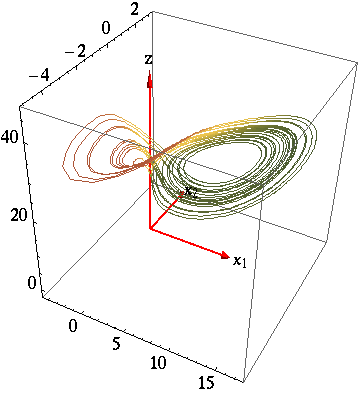
\includegraphics[width=0.40\textwidth]{CLEpcSect}
(b) 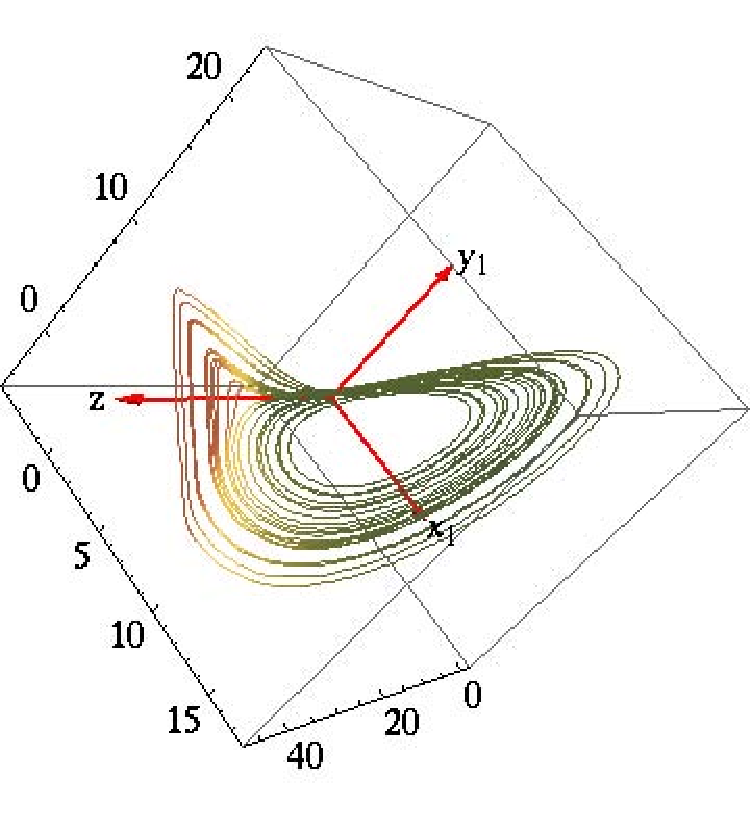
\includegraphics[width=0.43\textwidth]{CLEpcSect2}
\end{center}
\caption{
Method of moving frames, \slice\ fixed by a point on the \cLe\
\reqv\ group orbit, $\slicep  = \ssp_{\REQV{}{}1}$. The strange
attractor of \cLf\ %\reffig{fig:CLEx1x2z}
in the \reducedsp:
% of \refeq{EqMotionMovFramePC}:
(a) $\{x_1,x_2,z\}$ projection,
(b) $\{x_1,y_1,z\}$ projection.
Color-coding indicates $(\hat{\ssp} \cdot \hat{\slicep })_4$
where $\hat{.}$ stands for unit vector, with green indicating values
of the inner product close to $1$ and brown indicating values
close to $0$.
% \authorES
    }
\label{fig:CLEpcSect}
\end{figure}
%%%%%%%%%%%%%%%%%%%%%%%%%%%%%%%%%%%%%%%%%%%%%%%%%%%%%%%%%%%%%%%%
%
    \ES{I will add a scale in \reffig{fig:CLEpcSect} but it is too
   late here to do it tonight.}
    \PC{will need quality CLEpcSect, CLEpcSect2}
    \PC{ in \reffig{fig:CLEpcSect}:\\
        * Mark $\ssp_{\REQV{}{}1}$ \\
        * Draw stable eigenvector of $\ssp_{\REQV{}{}1}$\\
        * State value of $\ssp_{\REQV{}{}1}$ somewhere
        }
%
%%%%%%%%%%%%%%%%%%%%%%%%%%%%%%%%%%%%%%%%%%%%%%%%%%
% computed by PCunrot.nb
\SFIG{PCunrot1}
{}{
Method of moving frames, continuous time version, for the
polar coordinates motivated $x'=(0,1,0,0,z)$,
$x_1=0,\;x_2>0$, \slice. The \cLf\ strange attractor of \cLf\
% \reffig{fig:CLEx1x2z}
exhibits a discontinuity at
$x_2=0$ in the \reducedsp:
$\{x_2,y_2,z\}$ projection.
}
{fig:PCunrot1}
%%%%%%%%%%%%%%%%%%%%%%%%%%%%%%%%%%%%%%%%%%%%%%%%%%
%
Indeed, the method does encounter singularities in
subsets of \statesp.
For example, the \reducedsp\ equations \refeq{PCsectSin}
for the polar coordinates inspired \slice\
$x'=(0,1,0,0,z)$, $x_1=0,\;x_2>0$,
%this is illustrated by \reffig{fig:PCunrot}.
%$(\rho_1,\gSpace_1)$ are polar coordinates, $\rho_1 =
%\sqrt{\ssp_1^{ 2} + \ssp_2^{2}}$, see \refeq{eq:CartToPol},
are given by
%                                                    \exerbox{exer:csectionCLe}
\beq
\dot{\ssp} = \vel - \frac{\vel_1}{\sspRed_2} \, \sliceTan{}
\,,
\ee{EqMotionMovFrame1}
with phase velocity $\dot{\gSpace}$ divergent whenever $\sspRed_2$
changes sign, see \reffig{fig:PCunrot1}.


\item[J. Guckenheimer and A. Vladimirsky],
``A Fast Method for Approximating Invariant Manifolds,''
SIAM Journal on Applied Dynamical Systems
3, 232-260,
\\
http://www.math.cornell.edu/~vlad/papers/InvMfolds/InvMfold\_siads\_04.pdf
\\
is a potentially useful reference:
``The task of constructing higher-dimensional invariant
manifolds for dynamical systems can be computationally
expensive. We demonstrate that this problem can be locally
reduced to solving a system of quasi-linear PDEs, which can be
efficiently solved in an Eulerian framework. We construct a
fast numerical method for solving the resulting system of
discretized nonlinear equations. The efficiency stems from
decoupling the system and ordering the computations to take
advantage of the direction of information flow. We illustrate
our approach by constructing two-dimensional invariant
manifolds of hyperbolic \eqva\ in $R^3$ and $R^4$."

\item[F Giovannini and A Politi],\rf{GiPo91} might be worth a read:
\\
A method to compute the curvature of the unstable manifold is
introduced and applied to Henon map and Duffing attractor,
showing that it allows the authors to locate the homoclinic
tangencies and, in turn, to construct a generating partition.

It does not look like a good method (takes few values of a profile
for 1-d PDEs) but needs to be read nevertheless - also please
check its references, I have not noticed many of the papers:

\item[PC 2009-10-05]
looks like one should also read \refref{Abraham95}; they
report various return maps for \cLe.


also:
http://www.enm.bris.ac.uk/anm/preprints/2004r14.pdf

\item[Papers citing Christiansen \etal]
Read these papers  that cite \refref{Christiansen97}:
    \\
Misiurewicz and Zgliczynski\rf{MiZg01}
    \\
Zgliczynski and et al.\rf{ZgRi01}
    \\
Zimmermann\rf{zimmermann-global}



\end{description}

\section{2009-08-26 Method of slices for an $U(1)$-equivariant linear model}
\renewcommand{\ssp}{a}

%{\em \underline{Preamble:} My gut tells me that the method
%of moving frames, as described in the Section 4.2 of the
%thesis will \underline{not} work for KS.  But since my brain
%is dafter than my gut, I cannot explain why I feel that way.
%So, in order to make progress in this direction, I'm going to
%work with a dynamical system similar to KS, but much simpler.
%If I can figure out how to apply the moving frames to this
%system, then I can do it for KS as well.  If not, then I hope
%it will help me understand why my gut is right. \vspace{2ex}}

\medskip\noindent{\bf Ruslan} Forget \KS, let's consider a simpler dynamical system.
Let us say that, just like KS, we have a dynamical system on the space of real function $u(x,t)$ periodic in $x \in [-\pi, \pi)$, i.e. $u(x+2\pi,t) = u(x,t)$.  In the Fourier space $a = \mathcal{F}[u]$, $a = (a_1, a_2, \ldots)$, $a_k \in \mathbb{C}$ and $a_{-k} = a_k^\ast$.
I will also use polar coordinates, so $a_k = r_k \mathrm{e}^{i \phi_k}$.
The action of $U(1)$ on $u(x,t)$ is $g(\theta) u(x,t) = u(x+\theta,t)$. In the Fourier space
\[ g(\theta) a_k = \mathrm{e}^{ik\theta}a_k\,, \]
%In polar coordinates $\tau_{\shift/L} (r_k, \theta_k) = (r_k, \theta_k + q_k \shift)$.
To define the $U(1)$ group rotation tangent $t(a)$, we consider an infinitesimal rotation
\[ \mathrm{e}^{ik\theta}a_k = (1 + ik\theta)a_k  = a_k + \theta t_k\,, \]
so $t_k = ika_k$.
In matrix notation, $\mathbf{T} = \mathrm{diag}(ik)$,
    so  $t = \mathbf{T}a$.

The equation defining the slice through some point $\slicep$ is
\[ (\bar{a} - \sliceTan{}) \cdot \sliceTan{} = 0 \]
By the dot product we mean
\[ a \cdot b = \sum_{k=-\infty}^\infty a_k b_k^*\,, \]
which in the space of real periodic functions corresponds to
\[ f \cdot g = \int_{-\pi}^\pi f(x) g(x) dx\,, \]
where $f(x) = \mathcal{F}^{-1}[a]$ and $g(x) = \mathcal{F}^{-1}[b]$,
so this makes sense.  But note that this is not
the only way of defining the dot product.

\subsection{2009-08-26 Epicycles: 2-Fourier modes}
\label{sect:epyc2Fourier}

\medskip\noindent{\bf Ruslan}
Let us define a 2-Fourier modes linear dynamical system
$\dot{a}_k = v_k(a)$ as follows: $v_k = i \omega_k a_k$,
$\omega_{-k} = -\omega_k$, where $\omega_k \in \mathbb{R}$ are
constants.
    \RLD{$\omega_{-k} = -\omega_k$.
    I used this in my derivation to get the sign right.
    {\bf Predrag} Agreed - I used that too in rederiving your model.}
This
\HREF{http://www.c2.com/cgi/wiki?AddingEpicycles}
     {``epicycles'' model}
is a linear dynamical system, so we can solve it analytically:
\[ a_k(t) = a_k(0) \mathrm{e}^{i \omega_k t} \]
Even simpler, I'm going to use only the first two modes, so $a_k(0) = 0$ for all $|k| \neq 1$ or 2.

We can choose constants $\omega_1$ and $\omega_2$ such that this system can have
a traveling wave or a RPOs in the original space of periodic functions $u(x,t)$.\\
{\bf Example 1: \Reqv.} If $\omega_1 = c$ and $\omega_2 = 2c$, then
\[ a_k(t) = a_k(0) \mathrm{e}^{ikct} = g(ct) a_k(0)\,, \]
which is a wave traveling with speed $c$.\\
{\bf Example 2: \Rpo.} For the system to have an RPO, we can choose, for example,
$\omega_1 = \pi/2$ and $\omega_2 = 3\pi$.  This RPO has period $T = 1$ and shift $\pi/2$, since
\[ a_1(1) = a_1(0) \mathrm{e}^{i\pi/2} = g(\pi/2) a_1(0) \quad \mathrm{and} \quad
   a_2(1) = a_2(0) \mathrm{e}^{i3\pi} = a_2(0) \mathrm{e}^{i\pi} = g(\pi/2) a_2(0) \]

Let us now see what happens if we apply the method of slices to these two examples.
The reconstruction equation is
\[ \dot{\theta} = \frac{v(\bar{a}) \cdot \sliceTan{}}{t(\bar{a}) \cdot \sliceTan{}} \]
Let us say the initial condition $a_1(0) = r_1 > 0$, $a_2(0) = r_2 > 0$
(i.e. $\phi_1 = \phi_2 = 0$) is also the point $\slicep$ defining the slice.  Then
$\sliceTan{k} = ikr_k$ when $|k| = 1,2$ and zero otherwise.  So,
\beq
\dot{\theta} = \frac{\sum_k (i\omega_k \bar{a}_k) (ikr_k)^*}{\sum_k (i k \bar{a}_k)(ikr_k)^*}
                = \frac{\sum_k k \omega_k \bar{a}_k r_k}{\sum_k k^2 \bar{a}_k r_k}
\ee{RLDrec}
The equation for the flow on the slice (aka reduced flow) is
\beq
\dot{\bar{a}}_k = v_k(\bar{a}) - \frac{v(\bar{a}) \cdot \sliceTan{}}{t(\bar{a}) \cdot \sliceTan{}} t(\bar{a})
                   = i\omega_k \bar{a}_k - \frac{\sum_k k \omega_k \bar{a}_k r_k}{\sum_k k^2 \bar{a}_k r_k} ik\bar{a}_k\,.
\ee{RLDred}
\medskip\noindent{\bf Predrag}
I have coded \texttt{wilczak/matematica/PCruslan.nb} also for
$\slicep$ complex, if we need it - no reason to chose it real,
though experimentally it seems not to be the cause of the singularity in
$d\theta/dt$.

\noindent {\bf Example 1: \Reqv.} Here $\omega_k = kc$, so we immediately get
\[ \dot{\theta} = c \quad \mathrm{and} \quad \dot{\bar{a}}_k = 0\,, \]
as expected for the traveling wave.\\
{\bf Example 2:  \Rpo.} In general, for the flow with two non-zero
modes (remembering that $a_{-k} = a_k^*$ and $\omega_{-k} =
-\omega_k$):
\beq
 \dot{\theta} = \frac{\omega_1 r_1 (\bar{a}_1 + \bar{a}_1^*)
                  + 2\omega_2 r_2 (\bar{a}_2 + \bar{a}_2^*)
                  }{r_1(\bar{a}_1 + \bar{a}_1^*) + 4r_2 (\bar{a}_2 + \bar{a}_2^*)}
\ee{Period1}
and
\[ \dot{\bar{a}}_k = i\omega_k \bar{a}_k - \frac{\omega_1 r_1 (\bar{a}_1 + \bar{a}_1^*) + 2\omega_2 r_2 (\bar{a}_2 + \bar{a}_2^*)}{r_1(\bar{a}_1 + \bar{a}_1^*) + 4r_2 (\bar{a}_2 + \bar{a}_2^*)}ik\bar{a}_k \]
When $\omega_1 = \pi/2$ and $\omega_2 = 3\pi$, the second equation should generate a periodic orbit with period $T = 1$, while the solution of the first equation, starting with $\theta(0) = 0$, should give us $\theta(1) = \pi/2$.  Unfortunately, we cannot solve these equations analytically, so I'll do it numerically for different values of $r_{1,2}$.  I'll set $r_1 = 1$ and increase $r_2$ from zero.  Note that when $r_2 = 0$, we just have a traveling wave with speed $\omega_1$.  Also, when $r_2$ is sufficiently smaller than $r_1$, we will have a traveling wave slightly modulated by the 2nd mode.  This case is shown in the figure below:

\vspace{2ex}\noindent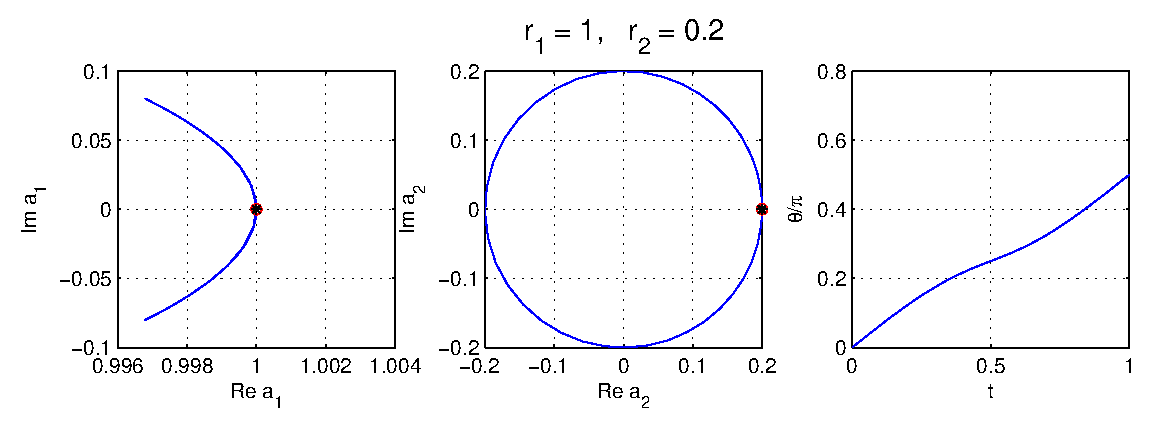
\includegraphics[width=\textwidth]{sliceflow1}

So, everything works well: the reduced orbit is periodic (the beginning of the orbit is denoted by the red circle, while the end is denoted by the black asterisk), and the phase shift at $t = 1$ is equal to $\pi/2$.  We can see similar picture when we increase $r_2$:

\vspace{2ex}\noindent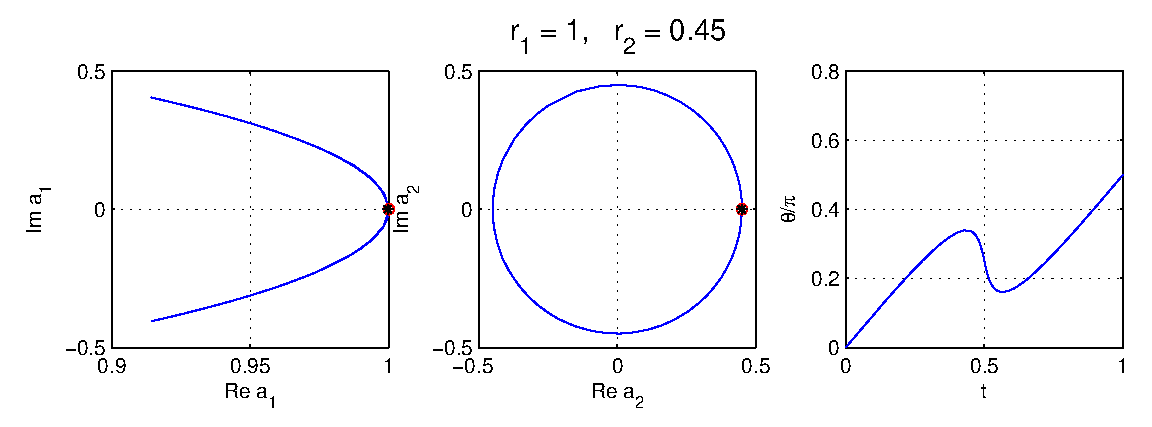
\includegraphics[width=\textwidth]{sliceflow2}

Now, when $r_2$ approaches 0.5, it is clear that the orbit approaches a singularity:

\vspace{2ex}\noindent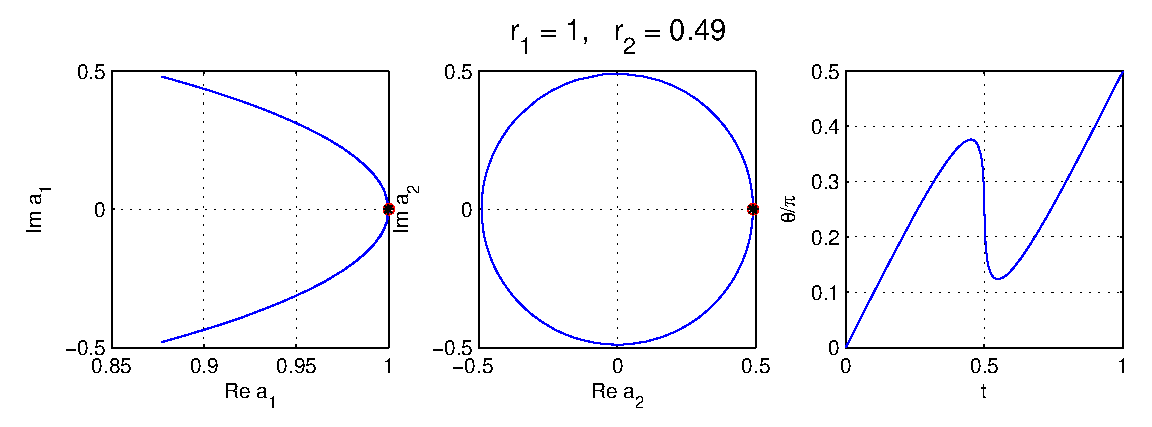
\includegraphics[width=\textwidth]{sliceflow3}

At $r_2 = 0.5$ we get rubbish:

\vspace{2ex}\noindent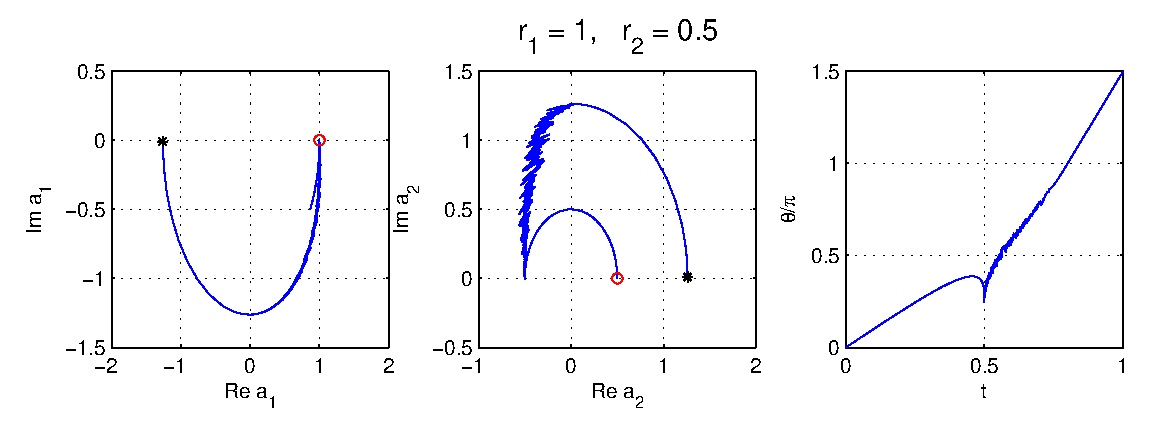
\includegraphics[width=\textwidth]{sliceflow4}

which persists for awhile

\vspace{2ex}\noindent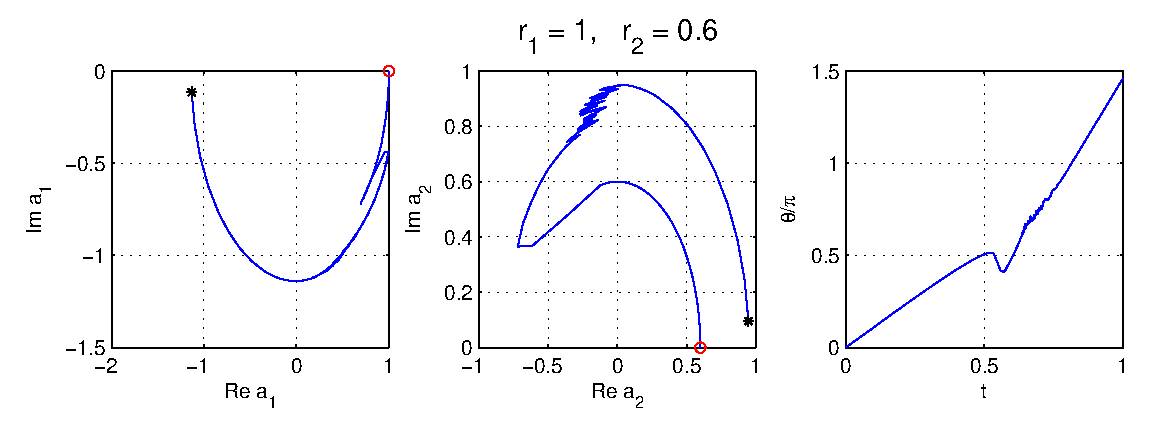
\includegraphics[width=\textwidth]{sliceflow5}

until we get back the nice smooth solution:

\vspace{2ex}\noindent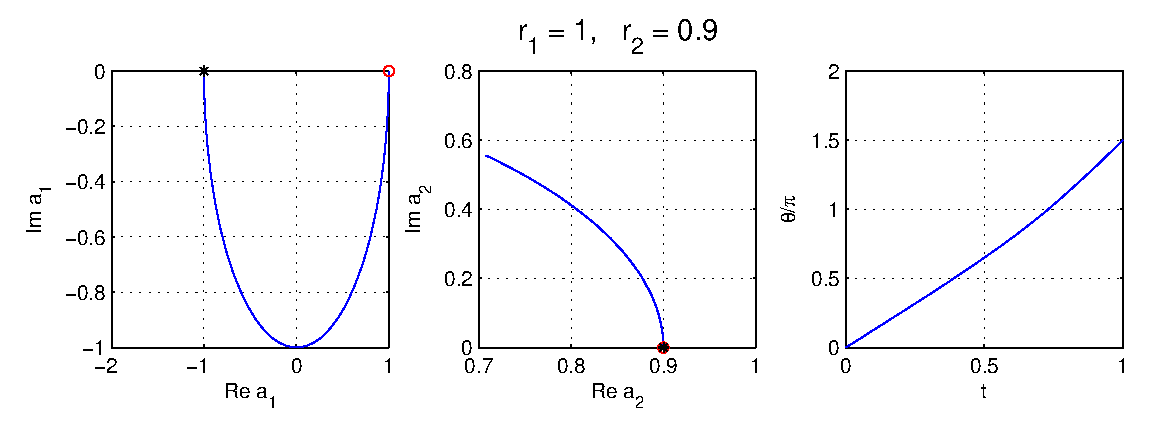
\includegraphics[width=\textwidth]{sliceflow6}

which, however, is no longer periodic, while the shift is now $3\pi/2$.  This picture persists for all $r_2 > r_1$.

\vspace{2ex}\noindent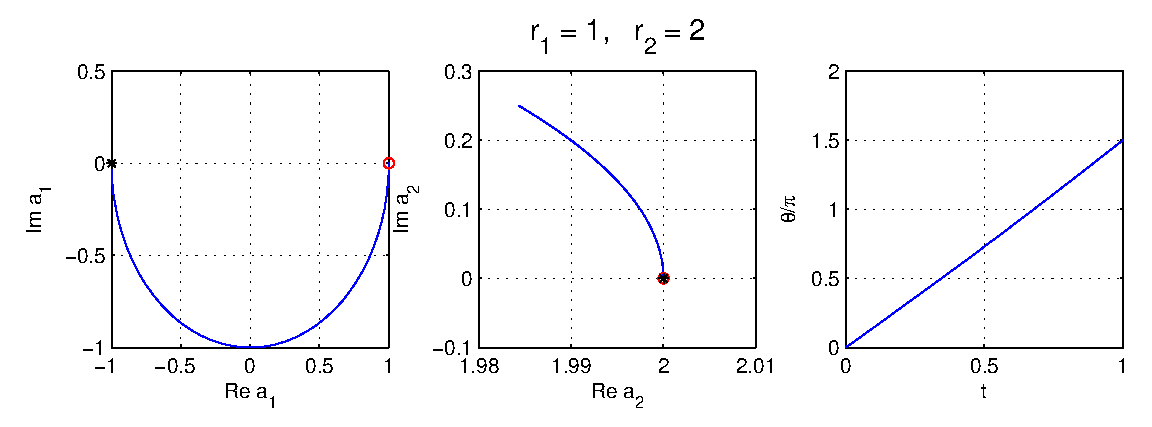
\includegraphics[width=\textwidth]{sliceflow7}

So, it looks like the problem with the method of slices is not only due to running into the singularities,
but also due to the possibility of generating smooth orbits which go around those singularities
and generate wrong shifts without any indication that something has gone wrong.
These orbits are no longer periodic in the reduced space.  The only time this method works
reliably is when the flow is dominated by the first Fourier mode.  If this is not the case,
as in the KSE regime with multiple active modes, then we cannot expect that it will work.~~{\em Q.E.D.}

\vspace{2ex}
An old idea presented as a new one:  Why don't we define the dot product in the above equations as follows:
\beq
 a \cdot b = a_1 b_1^* + a_1^* b_1
 \,.
\ee{RLDfix}
Then, if I'm not mistaken, the whole thing reduces to my original idea for factoring out the $U(1)$
symmetry from the KS flow.  In this case we won't need to worry about running into, or moving around,
the singularities while generating spurious phases.  The only singularity will be at $r_1 = 0$,
which is trivial to deal with.

With the dot product defined as in \refeq{RLDfix},
\refeq{RLDrec} and \refeq{RLDred} become
\[
  \dot{\theta} = \omega_1
  \quad \mathrm{and} \quad
  \dot{\bar{a}}_k = i(\omega_k - k\omega_1) \bar{a}_k
\,.
\]
So they (obvious to Ruslan) do the job.


\subsection{2009-08-25 Eurosceptics do not like to slice}
\noindent{\bf Ruslan} (Predrag's translation) one gets a
phase shift by $\pi$ if one crosses the singularity.
\\
{\bf Ruslan} The shifts by $\pi$ is the least of my worries.
It is the fact that when $r_2 > r_1$ we get a nice smooth
solution of the reconstruction and reduced equations, yet we
get obviously wrong results.  I don't want to think why this
is happening.  I'd rather just stop using the approach where
such a thing can happen.
\\
{\bf Predrag} Your model illustrates why we need
monotonicity in phase (we are integrating 1d equation,
velocity cannot change sign?). But I think we will fix it -
it is like WKB for harmonic oscillator, one gets geometric
$\pi$ phase for each turn, and a neat way to do it is Maslov
trick - change slice at $\pi/4$, then change back at
$3\pi/4$, etc. Looks like something we can figure out. Sure
cute - getting semiclassical Keller-Maslov phase without
doing neither wave nor quantum mechanics. At least, not
consciously.

More interesting will be the phase for the method of
connections. If we are lucky, it is the same for relative
periodic orbits.
\\
{\bf Ruslan} We had the discussion about monotonicity some
time ago (see above).  I don't have anything more to add at
the moment.
\\
I don't know much about WKB, or Keller-Maslov
phase, but I would like to get away from generating all kinds
of fixes, like using random $\slicep$ or switching between
slices.

\medskip\noindent{\bf Predrag} 1st mode will not work. Actually,
what Ruslan has run into so far is the same problem you
(Evangelos) and Rebecca run into independently; he is
measuring angle in polar coordinates, where we also run into
$d\theta/dt$ divergence, and shifts by $\pi$.
\\
{\bf Ruslan} I disagree that 1st mode won't work, I think it
will. And I don't think using polar coordinates is the
problem.  Forget about dynamics.  Just look at functions
defined on a circle and ask yourself how to identify
functions that differ only by a shift.  My answer: The phase
of the 1st Fourier mode will give you the shift.  So just use
it to rotate the functions on top of each other.

\noindent {\bf Evangelos} Apart from quantum mechanics there
are classical systems that exhibit such behavior, see for
example
\HREF{dx.doi.org/10.1103/PhysRevLett.103.034301}
{this PRL paper}. I've only seen it in Hamiltonian systems,
where this behavior is called monodromy since one studies the
system as it goes once around a singularity (is the etymology
clear to non-Greeks too?). It apparently arises when a
function fails to be single-valued, which again should point
out why we need monotonicity in phase.\\
\textit{Question for Ruslan} Is it really trivial to deal
with the singularity at $r_1=0$?\\
{\bf Ruslan} Yes, but you should never ever try to
numerically integrate the reconstruction or the reduced flow
equations if you expect to get the correct reduced
representation of the orbits of the original flow.  Instead,
integrate the original flow and then pull the obtained orbit
onto the slice while keeping track of the shift you generate
while doing it.  If the original orbit goes exactly through
$r_1 = 0$ (within the round-off error), then add (or
subtract) $\pi$.  That's all.\\
{\bf Evangelos}  I agree that integrating the equation on the
slice is not the safest think to do. I would like to
understand where the spurious shifts that you have discovered
come from, though. It looks like the reduced space has a
branch cut and as one integrates the equations around the
singularity he finds oneself on a different leaf.

There is something I don't understand in the procedure you
describe here. Does the need to add or subtract $\pi$ come
from the fact that most implementations of $arg$ or $arctan$
functions do not distinguish quadrants? I do not understand
how else it is connected to crossing through $r_1 = 0$ or why
it does take care of the singularity. You can approach the
singularity through any direction on the $a_1$ plane, so the
way to overcome the singularity on a point with $r_1=0$ seems
to be to use the angle at which you approach to it (that you
get from the previous point) to correctly rotate it onto the
slice. The difficulty is that then you are not able to tell
where $\EQV{2}$ and $\EQV{3}$ lie on this space as they both
have $r_1=0$: their group orbits do not intersect your slice,
so you do need another ``coordinate chart'' to cover the
space.
\\
{\bf Evangelos} You still need to cover the reduced space
with more than one coordinate systems which is essentially
the same as choosing a new slice.\\
{\bf Ruslan} No. You don't need more than one coordinate
system.  Just use the Fourier modes as reduced coordinates,
with the phase of the 1st mode fixed.  The phase of the 1st
mode will be the reconstruction shift.\\
{\bf Evangelos} Even if this doesn't bother us, I am afraid
that we will get projections that are not more informative
than Figure 42 in today's version of my thesis, where the
singularity was dealt with but $\EQV{2}$ and $\EQV{3}$
collapse to the same point.\\
{\bf Ruslan} I cannot guarantee that the pictures we get
will be nice and simple.  Of course, since the reduced space
is a semi-space (because $r_1 \geq 0$), the reduced orbits
may not always look pretty and smooth: They will have sharp
turns when they come close to, or hit, the $r_1 = 0$
subspace.  But at least when I look at orbits projected onto
Fourier modes, I know how to interpret them.  When I'm
looking at the projections onto some exotic curvilinear
coordinates, the pictures make no sense to me.\\
{\bf Evangelos} On the utility of Fourier modes as a
representation I disagree in two levels. I anyway find that
Fourier modes projection tell us very little about dynamics.
Wasn't this the reason to use different coordinate systems in
the KS paper? So as long we can construct dynamically
meaningful projections in the new variables I do not worry
how we got them.

Furthermore, what you describe above is equivalent to using
the invariants of Table 3 in Chapter 8 in my thesis. The new
coordinates are exactly the Fourier modes rotated back to the
slice defined by $\Im(c_1)=0$, this is how they were
obtained. The difference is that in Table 3 the singularity
is explicit. The important point though is that what you like
to see as a linear transformation is in fact a nonlinear
transformation through the dependance of the angle on the
point in space in which it is evaluated. Whereas in a linear
transformation all points in space are rotated by the same
angle. Therefore without knowing it you use exotic
curvilinear coordinates. The connection to the original
Fourier modes is that the magnitude in each Fourier plane
stays invariant. Of course things get even more exotic in my
thesis, but the motivation behind that was to get projections
that provide more information about the dynamics.

As a general comment, it appears that when we try to see the
reduced space as embedded in the original space, no matter
how we go from $N$ to $N-1$ dimensions we impose a
conservation law that did not exist in the original system
(as it was allowed to have motion in the direction of group
action) that restricts the motion to an $N-1$ dimensional
space which cannot in general be given a nice structure.

\subsection{2009-08-26 Eurosceptics carry the day}
\label{sect:2009-08-26}

\noindent{\bf Predrag} OK, now that Ruslan has gone on
strike I spent a day screwing around with Mathematica,
checked epicyclist formulas and reproduced Ruslan's graphs.
As I am using \texttt{NDsolve[\dots]} as a black box, I do
not get the same screwy details close to $(r_1,r_2)=(1,0.5)$,
but the result is the same - for $r_2$ sufficiently larger
than 1/2 one gets extra $\pi$ shift, with no integration hint
that one is going around a singularity. That is unacceptable.
As Ruslan expects,
random choices of complex (not real) \slice\ fixing
point $\sliceTan{}$ move the singularity around but are essentially no
help.

I will still try to use Maslov trick and switch the slice
whenever $\dot{\theta}$ starts misbehaving, but for that I
need to learn how to use \texttt{Method -> \{"EventLocator"}
within \texttt{NDsolve[\dots]}, but that sure looks like a
bitter pill. I do not mind having several slices as long as
the returns to (dynamical) Poincar\'e sections trace out
smooth unstable manifolds suitable to partitioning the
\reducedsp.

Marsdenites did not note this problem as they only applied
the method to \reqva, and there it is OK.

I agree that if one is to fix the \slice\ by one Fourier
mode, \refeq{RLDfix} is the most natural choice, and would be
easiest to explain in a publication. Unfortunately, we ran
into singularities when we tried it for \CLe\ in Siminos
thesis\rf{SiminosThesis} and
\HREF{http://ChaosBook.org/projects}
     {Rebecca's summer project}.
But Ruslan, please do give it a try.

\medskip\noindent{\bf Ruslan}
Actually, not really on strike, just reluctant to participate
in your, what I believe to be, futile efforts to apply all
kinds of fixes and patches to the approach which, I believe,
is fundamentally incurable when it comes to systems like KS
in a fully developed chaotic regime. [\dots]

\medskip\noindent{\bf Predrag} Fair enough - way too many fixes and
patches. We need to quotient the symmetry in order to figure
out the symbolic dynamics for KS and for plane Couette and
pipe flows. If something like \refeq{RLDfix} works it would
be nicer. The reason why we think it will not is that when we
use the polar coordinates-inspired \slice\ fixing point
$\ssp^{*}=(0+i,0, \cdots)$, $\Re\ssp_1=0,\;\\Im\ssp_1>0$
(which I believe for $U(1)$ version corresponds to fixing the
phase of the first Fourier mode) the \reducedsp\ equations
are given by
\beq
\dot{\ssp} = v - \frac{{\Im} v_1}{{\Re}\ssp_1} t(\ssp)
\,.
\ee{EqMotionMovFrame}
Trajectories shown in %\reffig{fig:PCunrot1}
Siminos thesis\rf{SiminosThesis} and
\HREF{http://ChaosBook.org/projects}
     {Rebecca's summer project}
exhibit jumps by $\pi$. With $\ssp^{*}$ on \reqv\ orbit we
were luckier, and got a strange attractor which encountered
no $\dot{\theta}$ singularity. But unhappy, as we did not
understand why we were lucky.

\subsection{2009-08-27 Don't worry. Be happy}

\begin{description}
\item[Ruslan]
    Let me start by answering Evangelos's question about rotation
by $\pi$.  Forget about multiple modes for the moment.  Just
consider evolution of the first mode: $a_1(t) =
r_1(t)\mathrm{e}^{i\phi_1(t)} \in \mathbb{C}$.  If $a_1(t)$
goes through zero, then $r_1(t)$ bounces off of zero, while
$\phi_1(t)$ changes by $\pi$ or $-\pi$, (the sign is
immaterial).   This is just the nature of the polar
coordinates and has nothing to do with the implementation of
$arg$.

\item[Evangelos]
But still I don't understand why would you need to add or subtract
$\pi$? Doesn't the function you use to calculate the angle in this
plane take care of that?

\item[Ruslan]
That's it.  All I was saying
was that $\phi_1$ would change by $\pi$ or $-\pi$ as $a_1$
crosses zero.  And that's what the angle function would give
you.  Nothing else needs to be added.

\item[Ruslan]
Now about the nature of what you call the 'singularity'.  If
I understand it correctly, what worries you is that, if we
take $\phi_1$ as our $\theta$, then each time it changes by
$\pi$, the $k$-th mode needs to be changed by $k\pi$, $k >
1$.  You perceive this as a jump, i.e. a discontinuity of the
reduced orbit, which you don't like.  Is this what you mean
by the 'singularity'? If `yes', then do you really need to
worry about it?

\item[Predrag]
If $1/x$ is considered a
`singularity' for $x=0$ on small islands off Continent, than
we will be so bold to call it singularity. As you say, there
should be simple analytic fixes for going through zero; we
have to make sure that we teach our numerical routines how to
implement this. Your pretty and clean epicycle model just
gave me a new set of ulcers, as for $r_2$ not very larger
than 1/2 the integrators seem not to know that there was any
singularity at all, and relative periodic orbits became
periodic only mod~$\pi$. And $\pi$ or $-\pi$  sign is not
immaterial - we have to get \rpo s shifts right.

\item[Evangelos]
I want to add that the singularities in expressions such as
in Table 3 in Chapter 8 of my
thesis cannot be essential, in the sense that, since the transformations
are generated by rotations, the expressions
cannot really blow up. In practice they pose numerical issues,
related to the small denominators in these expressions. So I agree there
should be simple analytic fixes.

\item[Ruslan]
If you think about it, what you perceive as a jump is
actually a very fast rotation (infinitely fast if you go
exactly through zero, but otherwise finitely fast).  If you
don't like that it rotates so fast, then why don't you just
rescale the time?  Just slow it down near $r_1 = 0$.  I think
something like $d\tau = dt/r_1(t)$ might work, since it will
remove $\Re\ssp_1$ from the denominator in
\refeq{EqMotionMovFrame}.

\item[Predrag]
Agreed. I have been also thinking about redefining time.
That's also in ChaosBook
\HREF{http://chaosbook.org/chapters/conjug.pdf} {Chapter 6 - Get straight},
called there the
Kustaanheimo-Stiefel (also known as KS!) transformation, and
applied in Example 6.2: what to do with Keplerian ellipses of
arbitrarily large velocity. That we might need for close
passages to the $U(1)$ invariant subspace, with $r^2 = \sum
\ssp_k^*\ssp_k$ going small. Fortunately, in KS that never
happens - strange attractor is safely away from the $u(x)=1$
\eqv. Our problem with method of slices is more naive, as you
explain above.

Of course, the real challenge is: who will be the first to read the
\\
\HREF{ChaosBook.org/projects/siminos/thesis.pdf}
      {Thesis that Nobody Reads} first?

\item[Ruslan]
On the other hand, if our goal is to eventually reduce the
dynamics to a Poincar\'e map, then why do we need to worry
about time at all?

\item[Predrag]
Agreed - anything that gets us the sensible return (or
forward) maps is good. Just have to make numerics is correct,
and yields correct \rpo s shifts and periods - at the moment
we do not know how to do that right even for the 2-mode
epicycles model.

\item[Evangelos]
I also agree, that was my thesis final conclusion on what one should do: just
make sure that the Poincar\'e section is away from problematic regions. It is
just that finding a good section is not always easy, so one needs some visualization
that works well in order to get intuition on where to place it.
\end{description}

\subsection{2009-08-28 On ulcers, singularities, and `tender beasts'}

\noindent{\bf Ruslan} I thought the dot product
\refeq{RLDfix} would cure your ulcers for the epicycle model,
and I'm pretty sure for the CL and KS as well, provided you
stop worrying about the fast rotations in the reduced space.
I don't mind that you call them `singularities', but, hearing
your complaints about numerics, I'm pretty sure somebody
does...  Let me tell you something about computers: they are
tender beasts and if you say, or even think, this word in
their presence, they will get spooked and throw all kinds of
fits.  But seriously, as I already said above, any symmetry
reduction or other transformations that you want to carry out
should be done as post-processing, i.e. after you obtain your
numerical trajectory by integrating the original flow.  That
way the singularities are much more tractable numerically.

\subsection{2009-08-27 Maslov trick}
\label{s:MaslovTrick}

\noindent{\bf Predrag}  The Maslov trick is described in
\HREF{http://chaosbook.org/version12/chapters/WKB.pdf}
{ChaosBook vers. 12, Chapter 31} - WKB quantization.
Now I realize I give no references to Maslov paper or other
relevant sources - if you find them, please let me know so we can
write up the remark on the Maslov approach. Citing from this
chapter:

A simple physical picture, due to Maslov, is illustrated by quantization
of the harmonic oscillator. Semi-classical propagator has
a factor $1/$(velocity$)^{1/2}$, reminiscent of our $\dot{\theta}$, and
that blows up at the turning points, points where the particle as viewed
from the $q$ coordinate frame reverses velocity.

In the $q$ coordinate, the turning points are defined by the
zero kinetic energy condition,
and the motion appears singular.
This is not so in the full \statesp: the trajectory in a smooth confining
1-dimensional potential is always a smooth loop,
with the ``special'' role of the turning points $q_L, q_R$ seen to be an
artifact of a particular choice of the $(q,p)$ coordinate frame
(in our application, choice of a slice). Maslov's
idea was to proceed from the initial point
$(q',p')$ to a point $(q_{A},p_A)$ preceding the turning
point in the $\psi(q)$
representation, then switch
to the momentum representation (in our application, use a slice turned by
$90^o$)
continue from $(q_A, p_A)$ to $(q_B, p_B)$, switch back to the coordinate
representation (in our application, use a slice turned by
$90^o$), and so on.

In other word, as slices are local, switch to the next one whenever
convenient, and for recurrent orbits, make sure you are in the original
slice when you come back, in order to get a return map and hopefully sensible
symbolic dynamics.

\subsection{2009-08-28 Any 2-mode epicycle reduces to a periodic orbit}

\begin{description}
\item[Predrag]
A generic 2-Fourier modes epicycle trajectory runs on a 2-torus in the
full \statesp. Hence any trajectory is a \po\ in the \reducedsp, not
only the hand-crafted \rpo\ such as \refeq{RLDrec}.
(I actually verified this statement by running random trajectories
in \texttt{Mathematica}, so it is true.)
For testing methods of symmetry reduction
it might be a good idea to increase the number of Fourier modes.
\item[Ruslan]
That's right.  And thinking about it
as a 2-torus might hint at why the singularity develops as
$r_2$ grows. As $r_2$ grows, at some point the torus becomes
self-intersecting. I'm sure this happens when $r_2 = r_1/2$.
The $\SOn{2}$ group orbit on this torus is a line that winds once
around $r_1$ and twice around $r_2$.  As the torus becomes
self-intersecting this orbit first self-intersects at $r_2 =
r_1/2$ and then forms a knot.  And that's why an extra $\pi$
shift appears when we try to project an orbit onto the slice
normal to this knot.  This is just a speculation, but maybe
there is something in it.
\end{description}

\section{2009-08-27 Symmetry reduction by method of connections?}

\noindent{\bf Predrag}
Here we take $t(\ssp)$ to
be the tangent for the trajectory state space point \ssp\ is
used \emph{locally}, within the `horizontal' hyperplane
normal to $t(\ssp)$.

The 2-epicycle model is a linear sum of Fourier modes
$(\ssp_{-2},\ssp_{-1},1,\ssp_1,\ssp_2)$.
Predrag's first guess for the reconstruction equation for
phase shift for slice fixed \emph{locally} by $t(\ssp) =
T\cdot\ssp(t)$ was
\beq
\frac{d\theta}{dt}=
     \frac{t(\ssp)^{*} \cdot \dot{\ssp}(t) + \dot{\ssp}(t)^* \cdot t(\ssp)}
                        {2 \,t(\ssp) \cdot t(\ssp)^{*}}
\,,
\ee{MethConnWrong}
which evaluates to
\[
\frac{\omega_1\, \ssp_1(t) \ssp_1(t)^{*}
  + 2\,\omega_2\, \ssp_2(t) \ssp_2(t)^{*}
     }{
               \ssp_1(t) \ssp_1(t)^{*}
  +         4\,  \ssp_2(t) \ssp_2(t)^{*}}
\,.
\]
This integrates to a convoluted, initial point dependent
but \po\ in the reduced
space, because in the 2-epicycle model all motion is on
2-torus in the full \statesp, 1-torus in the
$U(1)$-\reducedsp. The reconstruction equation
\refeq{MethConnWrong} appears to be wrong; I forgot to
include the `connection,' \ie, the effect of the frame itself
changing in the next time step. Presumably \stabmat\
needs to be included, as in the Lie algebra equivariance
condition
(see Siminos thesis\rf{SiminosThesis} and
\HREF{http://ChaosBook.org/projects}
     {Rebecca's summer project}).
For linear models \stabmat\ is constant, would be easy to
include into integrations.

If you want to be a path-breaking American type entrepreneur, rather
than a Eurosceptic kvetch, derive the right reconstruction equation
for this case. The glove is thrown.

\begin{description}
\item[Ruslan to Predrag]
I've never aspired to be an American entrepreneur.
I'm a lazy Ukrainian, so I don't do things unless I'm
convinced they are relatively easy to do and will result in
something useful.  Besides, I don't like algebra, not even of
Lie kind, not even of any kind.  I like geometry.  And the
vague picture I have in my mind tells me that the method of
connections, being in some sense more local than the method
of slices, has even less chance of succeeding where the
problems we are experiencing are clearly of a global nature.
So, I don't understand why I should be trying to work through
this quite complicated calculation, while I have a much
simpler approach based on the 1st Fourier mode, which works
for epicycles and I'm quite sure will work for KS.  It might
not give me a nice and smooth orbit.  The orbit might even
look ugly, but at least it will be a correct symmetry reduced
orbit.

\item[ to Ruslan]
OK, we'll suffer through
convoluted algebraic thinking as it applies to the geometry
of equivariant flows, and you industrious subject of Queen
Elizabeth go test \refeq{RLDfix}, the simple approach based
on the first Fourier mode, on KS.

\item[ to Predrag]
OK, this glove fits me better, especially since I've done most of it 20 months ago.
\end{description}

\section{2009-08-29 Kuramoto-Sivashinsky O(2) quotienting}

\subsection{Back to the future: pasting from 2007-12-31}

\medskip\noindent{\bf Ruslan pasting from siminos/blog/davidchack/071231fundamental.html}
To fix the notations, let me recap the Kuramoto-Sivashinsky
equation (KSE) and its representation in Fourier space:
\[ u_t = -uu_x - u_{xx} - u_{xxxx},  \quad x \in [-L/2, L/2] \]
with periodic boundary conditions:  $u(x+L,t) = u(x,t)$.  In the Fourier representation
\[ u(x,t)=\sum_{k=-\infty}^{+\infty} a_k (t) e^{ i q_k x }\,,\]
where $ q_k = 2\pi k/L$, the KSE takes the form
\[ \dot{a}_k = v_k(a) = (q_k^2 - q_k^4)a_k - \frac{iq}{2}\sum_{m=-\infty}^{\infty}
    a_m a_{k-m}\,,\quad a_k \in {\cal C}\]
It is convenient to represent complex modes as pairs of real
variables, either in cartesian or polar coordinates:
\[ a_k = (b_k, c_k) = b_k + ic_k = (r_k, \theta_k) = r_k e^{i\theta_k}\,. \]

\noindent{\bf Symmetries:} If $u(x,t)$ is a solution of the KSE, then so are
\[ \tau_{\shift/L} u(x,t) = u(x+\shift,t) \quad\mbox{and}\quad R\,u(x,t) = -u(-x,t).\]
The action of symmetry transformations on Fourier modes is as follows:
\[ \tau_{\shift/L} a_k = e^{iq_k \shift} a_k = (r_k, \theta_k + q_k \shift) \,,\qquad R\,a_k = -a_k^\ast = (-b_k, c_k)\,.\]

\subsubsection{Defining KSE quotient space $\pS/$O(2)} % (a.k.a. fundamental domain)}
\label{sect:RLDslice}

The KSE quotient space $\pS/$O(2) is defined in Fourier space as follows:
\begin{enumerate}
\item If $r_1 > 0$ then $\theta_1 = \pi/2$ and $\dot{\theta}_1 \leq 0$;
\item if $r_1 = 0$ then $\arg \dot{a}_1 = \pi/2$;
\item if $a_1 = \dot{a}_1 = 0$ then the KSE solution lives in
        the $L/2$-periodic invariant subspace, where $\pS/$O(2) is
        defined as above but for the 2nd mode;
\item and so on...
\end{enumerate}
So the quotient space $\pS/$O(2) consists of a hierarchy of
slices fixed by the $k$-th Fourier mode for the
$L/k$-periodic invariant subspace.

\begin{description}
\item[Predrag's comment] I do not find fixing a single
Fourier coefficient natural, and you pay for it by having to
deal with discrete shift symmetry subcases separately (fixing
higher $k$ Fourier coefficients).
\item[Ruslan's reply] I think it is completely natural that
for solutions symmetric by $L/k$ shift, we use the $k$-th
Fourier mode. Since functions in $L/k$-symmetric subspace are
invariant under KS dynamics, using $k$-th Fourier Mode in
$[0, L]$ is the same as using the 1st Fourier mode in $[0,
L/k]$.  Also note that, again because of the invariance of
these subspaces, the choice of the mode which defines
$\pS/$O(2) is fixed once and for all times by the initial
condition, so there is no need to jump between slices when
following the KS flow.
\end{description}

\subsubsection{Mapping KSE solutions to $\pS/\SOn{2}$}

Following Predrag's suggestion, I'll split the mapping of KSE solution to
$\pS/$O(2) into two parts:
\\
1) map to $\pS/\SOn{2}$ by translation $\tau_{\shift/L}$; 2) map from
$\pS/\SOn{2}$ to $\pS/$O(2) by reflection $R$.

\medskip\noindent{\em ...to be continued...}

%\vspace{2ex}\noindent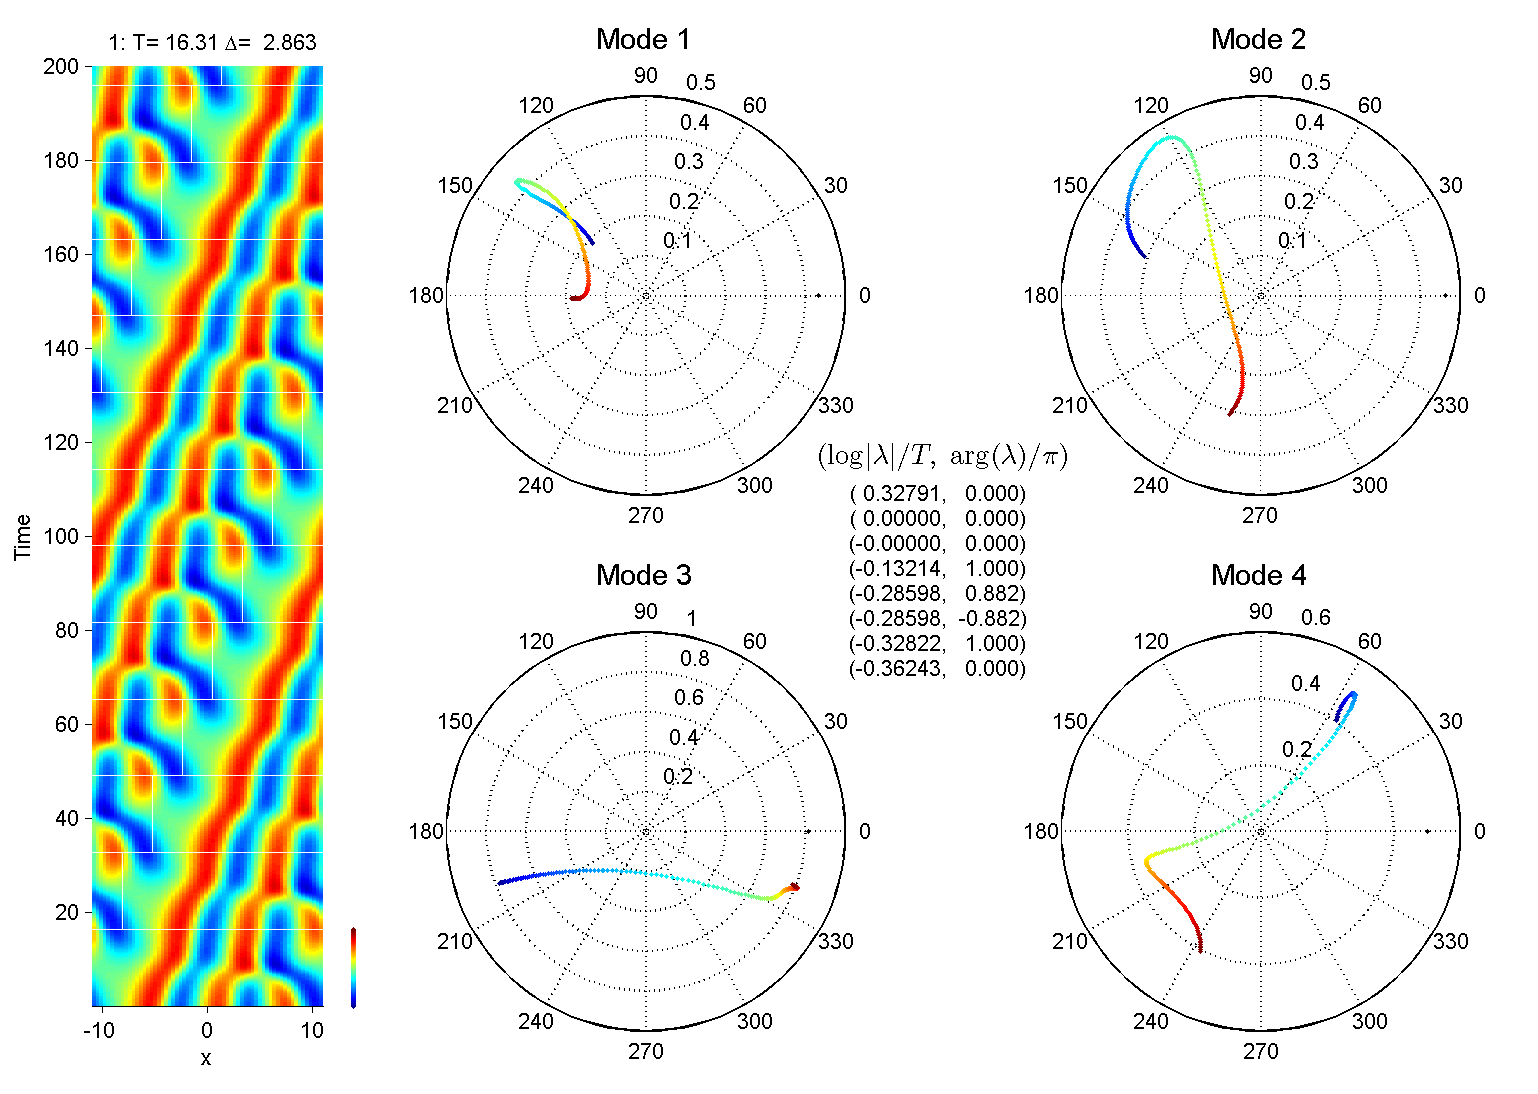
\includegraphics[width=\textwidth]{ks22rpo016.31_02.863.pdf}


%
% *Note 1:* The invariant subspace of antisymmetric solutions
%
% $$ u(x,t) = R\,u(x,t) = -u(-x,t) \quad\Rightarrow\quad Re\,a_k = 0 $$
%
% belongs to the FD.
%
% *Note 2:* If both
%
% $$ a_1 = 0 \mbox{~~and~~} \dot{a}_1 = 0 $$
%
% then the solution lives in the L/2-periodic invariant subspace, and the FD
% is defined in terms of
%
% $$ r_2 \mbox{~~and~~} \theta_2\,. \mbox{~~And so on...} $$
%
% A KSE solution
%
% $$ (r_1, \theta_1, r_2, \theta_2, \ldots) $$
%
% is mapped into the FD by translation
%
% $$ \shift/L = \frac{\pi/2 - \theta_1}{2\pi} $$
%
% and reflection if
%
% $$ \dot{\theta}_1 > 0\,, \mbox{~~or~~} b_1\dot{c}_1 - c_1\dot{b}_1 > 0\,, \mbox{~~since} $$
%
% $$ \dot{\theta_k} = \frac{b_k\dot{c}_k - c_k\dot{b}_k}{b_k^2 + c_k^2} $$
%
% The map into FD is characterized by two parameters: the translation
% parameter
%
% $$ \shift = \frac{\pi/2 - \theta_1}{2\pi}L $$
%
% and the reflection parameter
%
% $$ \rho = 1 \mbox{~~when~~} \dot{\theta}_1 \leq 0 \mbox{~~and~~} -1
% \mbox{~~when~~} \dot{\theta}_1 > 0 $$
%

\subsection{2009-08-31 A closer look at the singularity}

\noindent{\bf Evangelos}
Taking \CLe\ as an example I will examine how the invariants
\beq
\begin{split}
        \overline{x}_2 &= \sqrt{x_1^2+x_2^2} \continue
        \overline{y}_1 &= \frac{x_2 y_1-x_1 y_2}{\sqrt{x_1^2+x_2^2}}\continue
        \overline{y}_2 &=\frac{x_1 y_1+x_2 y_2}{\sqrt{x_1^2+x_2^2}}\,.
        \label{eq:invLaser}
\end{split}
\eeq
generated by straightforward application of the moving frame method behave as $x=x_1+i x_2$ approaches
zero. For the limit to exist we must get a direction independent result as $x\rightarrow 0$.
Using $x=r_x\, e^{i\theta_x}\,,\, y=r_y\, e^{i\theta_y}$ we can write, for instance, $x_2 y_1-x_1 y_2 = r_x r_y \sin(\theta_x-\theta_y)$
and therefore,
\beq
        \overline{y}_1= r_y\sin(\theta_x-\theta_y)\,.
\eeq
Therefore, for any given $y$, the limit of $\overline{y}_1$ for $x \rightarrow 0$ does not exist, as the above expression depends on the direction
on the complex $x$-plane along which we approach zero. In terms of projecting dynamics on variables \refeq{eq:invLaser} (or applying the equivalent
procedure of rotating points back to the \slice) this means that
we need to take into account the direction along which
we approach zero and use the `angle
of descent' as the angle with which we rotate points back to the \slice, if such points have exactly $x=0$ (in CLE this does not happen). Since the subspace $x=0$ is not flow invariant we do not need to worry about dynamics that stay within the subspace. We need to worry about the equilibria that exist in this subspace though, here the equilibrium at the origin, as there is no way to transform them to the new variables. For KS $\EQV{2}$ and $\EQV{3}$ belong to such a subspace.

\begin{description}
\item[Ruslan's more optimistic view of the singularity] Of
course, when $x = 0$, the angle $\theta_x$ is undefined.  But
if you look dynamically at $x(t)$ as it crosses zero at $t =
t_0$, then you realize that if $\theta_x(t < t_0) = \theta$
then $\theta_x(t > t_0) = \theta + \pi$ and all you need to
decide is how to define $\theta_x(t_0)$.  The most natural
definition is based on the direction of $\dot{x}(t = t_0)$,
i.e. $\theta_x(t_0) = \arg \dot{x}(t_0) = \theta + \pi$.
That's the reason I have item 2 in my definition of $M/$O(2)
quotient space.  So, as you can see, $\theta_x(t)$ remains
well defined at all times.

Regarding E2 and E3 in KS, they live in $L/2$- and
$L/3$-periodic subspaces, respectively.  So, to map them onto
$M/$O(2), we'll use the 2nd and 3rd Fourier modes,
respectively, as stated in items 3 and 4.

\item[Evangelos]
I agree about trajectories that cross zero, but not about
\EQV{2} and \EQV{3}. As soon as you use 2nd and 3rd Fourier
modes you effectively use different transformations, so it is
not obvious to me how you can piece everything together in
the same space. Fortunately we are not interested on dynamics
in $L/2$- and $L/3$-periodic subspaces, as they are not
invariant, but rather on how unstable manifolds of \EQV{2}
and \EQV{3} organize the $L$-periodic space. As those
unstable manifolds do not have vanishing first Fourier mode
we can visualize them and forget the equilibria.

\item[Ruslan]
  Actually, it's somewhat the other way
around for me: what worries you, does not worry me and vice
versa.  The proposed hierarchy of transformations is
completely consistent, since the higher-mode transformations
only act on those {\statesp} points which are not influenced
by the 1st mode transform.  By the way, the $L/k$-periodic
subspaces \underline{are} invariant: e.g. if $a_1(0) = 0$ and
$\dot{a}_1(0) = 0$ then $a_1(t>0) = 0$, so the solution is
$L/2$-periodic (provided $a_2(0) \neq 0$).  And finally, we
do have to keep track of the special symmetries of the
unstable manifolds of the equilibria.  For example, once
$\EQV{2}$ is placed within $M/$O(2) using the 2-nd Fourier
mode, its unstable manifold completely lives in the
anti-symmetric subspace (i.e. $Re\,a_k = 0$). {\color{blue}
The 1st mode transformation doesn't do anything to it, since
for any point on the manifold $\theta_1 = \pi/2$ already.}
So, the manifold we show in our SIADS Fig.~5.6 is already in
$M/$O(2).  What worries me is that $\EQV{2}$ is represented
here by two different points ($\EQV{2}$ and
$\tau_{1/4}\EQV{2}$).  This is the result of the additional
symmetry of $\EQV{2}$.  Whether or not these two points can
be merged into one $\EQV{2}$ without loss of dynamical
information about the KS flow, remains to be investigated.

What I wrote above, highlighted in blue, is wrong.  $\SOn{2}$
still acts in the antisymmetric subspace, since the points
there can also have $\theta_1 = -\pi/2$.  So they are rotated
by $\pi$.  Whether or not this will also rotate
$\tau_{1/4}\EQV{2}$ into $\EQV{2}$ I'm not yet sure.

\item[Evangelos]
$\SOn{2}$ does not act in the antisymmetric subspace (in the
sense that it does not leave it invariant as a set) but
merely on the intersection of antisymmetric subspace and its
$\tau_{1/4}$ translated copy. The group orbits of points on
antisymmetric subspace produce a family of copies of it. One
can identify a single representative by choosing for instance
$\theta_1=\pi/2$, so I don't see any problem with points on
the unstable manifolds of $\EQV{2}$. $L/k$-periodic subspaces
\underline{are not} invariant: if $a_1(0)=0$ then in general
$\dot{a}_1(0)\neq 0$, due to the nonlinear terms. Right?

\item[Ruslan]
  I didn't quite understand your
comments about the translated copies of the antisymmetric
subspace, but if you think it's not causing any problems, I'm
happy.  Regarding the $L/k$-periodic subspaces, I guess I
wasn't defining them correctly.  So, if $\dot{a}_1 \neq 0$
then we can still map this point to $M/$O(2) using the 1st
mode.  I was speaking then about the parts of $L/k$-periodic
subspaces which remain invariant under the KS flow.  They
need to be mapped to $M/$O(2) using higher FMs.

\end{description}


\subsection{2009-08-29 - Implementation of Ruslan's $a_1$-fixed slice}

\noindent{\bf Evangelos}
I thought its time to shut up and compute something, so I've
implemented first part of (my interpretation of) Ruslan's
prescription for KS that should take care of $\SOn{2}$. Namely,
I have fixed the \slice\ following
the rules of \refsect{sect:RLDslice}:
\bea
\Im \bar{a}_1  &=& 0
\continue
\mbox{If } r_1 &>& 0\,,\quad \mbox{\ESedit{rotate to the \slice\ by}}
        -\arctan( \Im a_1/\Re a_1 )
\continue
\mbox{If } r_1 &=& 0\,,\quad \mbox{\ESedit{rotate to the \slice\ by}}
        -\arctan( \Im \dot{a}_1/\Re \dot{a}_1 )
\,.
\label{ES-RLDslice}
\eea


\begin{figure}
 (a)~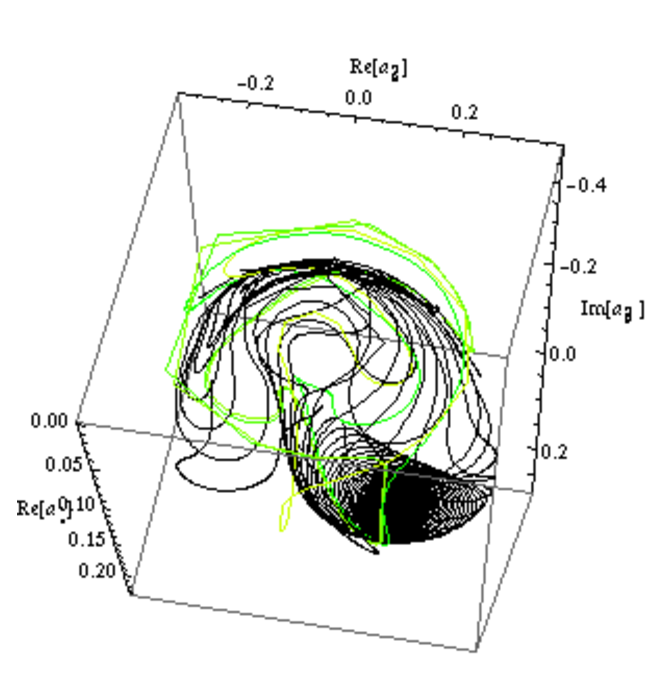
\includegraphics[width=0.45\textwidth]{ksRotatedTW1um}\,
 (b)~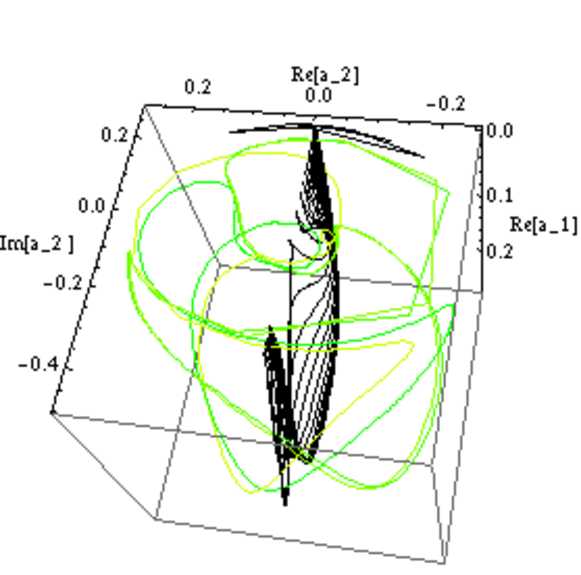
\includegraphics[width=0.45\textwidth]{ksRotatedE2um}
\caption{
 $(\Re \bar{a}_1,\,\Re \bar{a}_2,\Im \bar{a}_2)$ projections of KS
 $\SOn{2}$-reduced dynamics by slice \refeq{ES-RLDslice}.
 Several \rpo s are shown along with the
 unstable manifolds of (a) \REQV{+1}, (b) \EQV{2}. $L=22$.
}
\end{figure}

I've posted such a figure long ago in Jonathan's blog, but
nobody got interested. I am also not happy with this figure
but one might argue that there are implementation problems,
and this is probably right, so I will have a second look.
Then, if I am to follow Ruslan's next step in the
prescription and set $\Im \bar{a}_2 =0$ in order to include
$\EQV{2}$ in this figure, the equilibrium will not ``meet''
it's unstable manifold, correct?

\begin{description}
\item[Ruslan]
 I agree that the unstable manifold of $\EQV{2}$ reduced by
 the 1st mode to $\pS/\SOn{2}$ will not meet $\EQV{2}$ reduced by
 the 2nd mode. \par I have a question: do we expect that an
 antisymmetric solution of KS will remain antisymmetric in
 $\pS/\SOn{2}$?  If yes, then we are in trouble, which has
 nothing to do with using the 1st mode: As I stated above,
 the only thing $\SOn{2}$ can do to leave an antisymmetric
 solution antisymmetric is rotate it by $\pi$.  However, in
 order for the unstable manifold of $\EQV{2}$ (which is
 antisymmetric) to return to back to $\EQV{2}$ we need the
 rotations along the orbit to add up to $-\pi/2$ (to
 compensate for the $\tau_{1/4}$ shift).  So, somewhere along
 the way the unstable manifold has to leave the antisymmetric
 subspace.  This doesn't seem natural, since antisymmetric
 subspace is invariant under KS flow.

\item[Evangelos]
If we all agree that rotating points back to the slice $\Im\
a_1=0$ is equivalent to transformations of Table 3 in Chapter
8 in my thesis (that I copy here for convenience), up to
treatment of points with $a_1=0$, then my answer would be as
follows: applying reflections generated by $b_i\mapsto - b_i$
to the $u_i$ of \reftab{tab:SO2n6} we have $u_3\mapsto -u_3$,
$u_4\mapsto u_4$, $u_5\mapsto u_5$, $u_6\mapsto -u_6$ and so
on, so that the reflection matrix $\mathbf{R}$ in new
coordinates is diagonal, with entries $\pm 1$ and therefore
satisfies $\mathbf{R}^2=1$, as it should. Points in the
antisymmetric subspace $b_i=0$ for every $i$, are mapped to
points in the new coordinates that only depend on the $c_i$'s
and are therefore invariant under reflections, \ie,
antisymmetric. I don't see why the unstable manifold in
reduced space should leave the antisymmetric subspace, since
we don't even know were the equilibria live in such a reduced
space.

    \PCedit{
\item[Evangelos: 2010-04-05]
We can compute invariants in \reftab{tab:SO2n6} at least to
dimensions of order 100, I've computed some 256 invariants
for KS. It's just pointless to use more than order 10 for
L=22. BUT: They are not a Hilbert basis for the given action
of \SOn{22}, as they do not span the space. Specifically they
do not span the discrete cyclic subgroup isotropy subspaces
$Fix(C_q)$, for any $q$, as the transformations are not
defined for $a_1=b_1=0$. This should be an example for
Cartan's moving frame method.
    }


\item[Ruslan]
Well, we do know that the unstable manifold of $\EQV{2}$
converges to $\tau_{1/4}\EQV{2}$.  And I also assume that we
want $\EQV{2}$ and $\tau_{1/4}\EQV{2}$ to be represented by
the same point in the reduced space.  So, in order to bring
these two points together in the reduced space, we need to
rotate $\tau_{1/4}\EQV{2}$ by $-\pi/2$.  This rotation needs
to occur somewhere along an orbit (a closed loop in the
reduced space) within the unstable manifold of $\EQV{2}$.
But since the antisymmetric subspace is \underline{not}
invariant wrt rotation by $-\pi/2$, the orbit must leave the
antisymmetric subspace.  Another way to put this, is that, if
we only look at KS solutions within the antisymmetric
subspace, then $\EQV{2}$ and $\tau_{1/4}\EQV{2}$ are two
\underline{distinct} equilibria, since the first one is
unstable, while the second one is stable.  So, there is no
way to map these two equilibria into the same point while
staying within the antisymmetric subspace.

I don't know how much we should care about this, but this
tells me that, no matter how we construct the reduced space,
we will not be able to retain the simple structure of the KS
invariant subspaces within the reduced space.

\item[Ruslan 2009-10-14]
I still don't see how to reconcile this: On the one hand, it
would appear natural that the antisymmetric subspace should
be a part of $\pS/\SOn{2}$, but, on the other hand, the
antisymmetric subspace contains two distinct images of
$\EQV{2}$, while, in the reduced representation of the full
KS flow, we would hope that there would be only one point for
$\EQV{2}$ in $\pS/\SOn{2}$.  I can see only two possibilities
here: either we introduce discontinuities of the flow in
$\pS/\SOn{2}$ (like it is happening with my Fourier modes
representation), or we collapse the dynamics to a subspace
that completely ignores the phase information (e.g., like in
the energy transfer representation).

\item[Predrag 2009-10-15]
Yes, please quotient the full $\pS/\On{2}$. It's good to do so,
quotienting discrete symmetries helps a lot, see
\\
\wwwcb{/chapter/discrete.pdf}.

\item[Ruslan 2009-10-14]
Since I don't like collapsing things (I would like to have a
representation where I can keep track of the phase shift
$\theta$, which will allow me to reconstruct the original
dynamics if I wish to do so), and since I don't know how to
get rid of the discontinuities otherwise, I'm going to go
crazy and embrace them.  So, my plan here is as follows:
I'll try to construct a reduced representation (and hopefully
a Poincar\'e map) for the dynamics in the vicinity of the
unstable manifold of $\EQV{2}$. I think that if I manage to
do it here, then there is hope that it can be done for the KS
flow elsewhere as well.  I may continue using the Fourier
modes, or I might try something else, like using the
real-space representation (remember those $u$-$u_x$-$u_{xx}$
plots?).

\item[Predrag 2009-10-15]
You keep track of discrete $\LieEl$ for a given full
\statesp\ trajectory by noting every time you need to apply
it, upon exit from the fundamental domain, see Lorentz flow
$\pS/\Ztwo$ Van Gogh attractor in
\wwwcb{/chapter/discrete.pdf}.


\item[Evangelos to Ruslan]
Sorry that it took so long to get back to you, I am
just not sure I follow your arguments and I am afraid there
is a danger that the discussion becomes cyclic. The
antisymmetric subspace is indeed not invariant under $\pi/2$
rotations. On the other hand the image of the unstable
manifold of \EQV{2} under symmetry reduction by
\refeq{ES-RLDslice} is unique. It belongs to a
``antisymmetric set'' in the reduced space, in which space the
action of reflections has been properly re-defined as in my
previous post. Of course the latter set is not invariant
under the action of reflection as defined in the original
space. In other words, if we would like to see the reduced
space as embedded in the original space we would have to say
that the linear antisymmetric subspace has been deformed in a
nonlinear manner through the transformations in
\reftab{tab:SO2n6} and reflections no longer leave it
invariant. Then I do not see any problems with identifying
all copies of \EQV{2} with a single point. I just see greater
problems with a discontinuous $\pS/\SOn{2}$.

Regarding ignoring phase information. I think we both agree
that it is safer to integrate only in the original space. So
no matter how we construct the reduced space we do not need
to through away any information.


\item[Ruslan to Evangelos 2009-10-14]
I think you nailed it: The transformations that identify all
copies of \EQV{2} with a single point do not appear to
respect the reflection symmetry.  If that's the case then how
can you call it an 'antisymmetric subspace', if it's not
invariant under reflections?  I thought that this is how we
define the antisymmetric subspace in the first place (i.e.
that it's invariant under reflections).  Is it not so?


\item[Evangelos: 2009-10-16]
I call it antisymmetric only because points in the original
antisymmetric subspace are mapped to it. The correct term
would be the fixed point subspace of reflections
$\hat{\Refl}$ in the reduced space with coordinates $u_i$,
where now reflections $\hat{\Refl}$ are not defined in the
same way they are for the Fourier modes, but rather as in my
post of 2009-08-29. Perhaps it might help to have a look at
\reffig{fig:SO2inv}(a). There we can see that we still have
reflection symmetry. For instance the traveling waves come in
pairs. Points on the antisymmetric subspace are mapped on
points with $u_3=0$ in this projection. Of course this is a
projection on a modified set of invariants, but the idea is
the same.


\item[Ruslan: 2009-10-17]
OK, now I see where we differ.  I was hoping, maybe naively,
to find, for any $u(x) \in \pS$, a unique shift $\theta(u)$
such that $\tau_{\theta(u)} u(x) = u(x - \tilde{L}\theta(u))
\in \pS/\SOn{2}$.  I was also hoping that the shift could be
chosen such that $\theta(u) = 0$ (or $\pi$) for an
antisymmetric $u(x)$.  That's what I meant when I was saying
that my hope was that the antisymmetric subspace would belong
to $\pS/\SOn{2}$.

The phase of the 1st Fourier mode is doing the job quite
well, until we get to the point where $r_1 = \dot{r}_1 = 0$.
There I though I could use the 2nd Fourier mode, but
encountered the problem when looking at the unstable manifold
of \EQV{2}.  This manifold is antisymmetric, but it links two
points of \EQV{2} shifted by $\pi/2$ with respect to one
another.  So, I cannot construct $\theta(u)$ such that
$\theta(u) = 0$ (or $\pi$) in the antisymmetric subspace and
which identifies all \EQV{2} with a single point in
$\pS/\SOn{2}$.  And that's my dilemma...


\end{description}


\begin{table}[t]
\caption
{First $11$ fundamental invariants for the standard action
  of $\SOn{2}$}
\scriptsize
\[
\begin{array}{ll}
  u_1=r_1=\sqrt{b_1^2+c_1^2}&  \\ u_3=\frac{b_2 \left(b_1^2-c_1^2\right)+2 b_1 c_1 c_2}{r_1^2}&u_4=\frac{-2
b_1 b_2 c_1+\left(b_1^2-c_1^2\right) c_2}{r_1^2}\\ u_5=\frac{b_1 b_3 \left(b_1^2-3 c_1^2\right)-c_1 \left(-3
b_1^2+c_1^2\right) c_3}{r_1^3}&u_6=\frac{-3 b_1^2 b_3 c_1+b_3 c_1^3+b_1^3 c_3-3 b_1 c_1^2 c_3}{r_1^3}\\ u_7=\frac{b_4
\left(b_1^4-6 b_1^2 c_1^2+c_1^4\right)+4 b_1 c_1 \left(b_1^2-c_1^2\right) c_4}{r_1^4}&u_8=\frac{4 b_1
b_4 c_1 \left(-b_1^2+c_1^2\right)+\left(b_1^4-6 b_1^2 c_1^2+c_1^4\right) c_4}{r_1^4}\\ u_9=\frac{b_1
b_5 \left(b_1^4-10 b_1^2 c_1^2+5 c_1^4\right)+c_1 \left(5 b_1^4-10 b_1^2 c_1^2+c_1^4\right) c_5}{r_1^5}&u_{10}=\frac{-b_5
c_1 \left(5 b_1^4-10 b_1^2 c_1^2+c_1^4\right)+b_1 \left(b_1^4-10 b_1^2 c_1^2+5 c_1^4\right) c_5}{r_1^5}\\ u_{11}=\frac{b_6
\left(b_1^6-15 b_1^4 c_1^2+15 b_1^2 c_1^4-c_1^6\right)+2 b_1 c_1 \left(3 b_1^4-10 b_1^2 c_1^2+3 c_1^4\right) c_6}{r_1^6}&u_{12}=\frac{-2
b_1 b_6 c_1 \left(3 b_1^4-10 b_1^2 c_1^2+3 c_1^4\right)+\left(b_1^6-15 b_1^4 c_1^2+15 b_1^2 c_1^4-c_1^6\right) c_6}{r_1^6}\\
\end{array}
\]
\label{tab:SO2n6}
\end{table}

\section{2009-10-20 Blogging on}

\begin{description}
\item[2009-10-20 Predrag] Moved Lyapunov stuff to
    \refchap{s:LyapunovVec}

\item[2009-10-28 Evangelos to renormalization experts]

One of my border ideas: Repeat the process that led to the
invariants of \reftab{tab:SO2n6} in each irreducible subspace
$i$, \ie, apply the moving frame method by setting $c_i=0$ for
each $i$, producing invariants $u_k^i$ where $k$ labels
coordinates. Then $\sum_k u_k$ will be a set of linearly
independent invariants. We would be able to map all equilibria
to unique points in this basis if it where not for the
singularities at $b_i=c_i=0$ for every $i$. So we will need to
follow a regularization procedure to remove it, but it might
now be done in a more natural way than simply manipulating the
denominator. It just reminds me of procedures in which each
term in a sum diverges but the sum can be regularized. Fels and
Olver\rf{FelsOlver99} use regularization techniques for group
actions but it is too technical for me.

The practical problem is that I do not get the simplifications
that led to simple expressions in \reftab{tab:SO2n6} when I try
to apply the moving frames method with $i>1$, I have no idea
why. So in thesis I add in appropriate places the invariants we
know that we will always get, \ie\ the Fourier magnitude in
each subspace.

\item[2008-11-20 Predrag] Idea: a conserved quantity $\to$
continuous symmetry. Can one use Noether theorem?
[2010-01-07 Predrag incorporated in ChaosBook]

\item[2008-11-20, 2009-10-29  Evangelos] I think that we
unfortunately cannot use it for dissipative systems. Noether's
theorem applies provided we can formulate the system as a
variational problem. It has caused me a great deal of confusion
tending to think of symmetries in this Noetherian way even for
dissipative systems. Some recent progress(?) beyond Noether's
theorem is summarized by Bluman\rf{Bluman07} in
\arXiv{math-ph/0511035}. See also \refref{BlumanAnco02}.

\item[2010-12-06 Predrag]
Arnol'd, Kozlov and Neishtadt\rf{ArKoNe88}, p.~78 version of
Noether's theorem is so compact that it looks like we should be able
to find the first (or cyclic) integral of motion for every 1-continuous
parameter Lie symmetry. However,
\HREF{http://webusers.physics.uiuc.edu/~goldbart/PostScript/MS_PG_book/bookmaster.pdf}
{Stone and Goldbart}\rf{StGo09} discussion
in Sect 1.3.2 makes it simple and pretty clear that indeed a variational
formulation is a prerequisite.

\item[2009-10-31 Predrag] Bluman\rf{Bluman07} seems to be a clear
and useful reference. Noether
theorem requires that equations of motion be cast in Lagrangian form,
and that the Lagrangian exhibits variational symmetries.
Variational symmetries are hard to find. For a system of equations
to be variational in form requires that their number is even,
that its linearized system (Fr\'chet derivative) is self-adjoint,
and that the system is non-dissipative. Bluman gives examples of some
of the usual tricks to recast the system in variational form, and
then circumvents it altogether. Then he discusses how to work without
Lagrangians, but whether this could be of use to us is not at all obvious;
most unlikely. It would have already been done for KS, if there
was something to do...

\item[2009-10-30 Predrag] An idea(?). In all ``Lyapunov
analysis'' workshop contributions of \refsect{iscpif} the
isolated hyperbolic eigenvalues appear in multiplets which
reflect the symmetry of the dynamics; doublets for KS, quartets
for complex Landau-Ginzburg, singlets to quartets for the
2-dimensional hard ball gasses, depending on the number of
translational symmetries. Due to the nonlinearities, they are
not exact multiplets, and in the ``physical'' spectrum they are
mixed up. What happens if we compute the Floquet eigenvectors
in the \reducedsp\ $\pS/\Group$? That has no symmetry, and thus
no multiplets? Perhaps the \monodromyM\ factors the way it
factors for the \Fd s of evolution operators (as in the famed
unpublished paper, still not understood by anyone but its
author)?

\item[2009-10-30 Predrag]
Kalman filters were extensively discussed in ``Lyapunov analysis''
workshop weathermen contributions of \refsect{iscpif}, and in many other
places - perhaps . They are a clever way (at the level of assuming that
noise is Gaussian) of including partial observations into predictive
models. Here is why we might need them: in pipe flows, the 3-dimensional
velocity field is measured instantaneously by PIV in a 2-dimensional
section across the pipe, not in a 3-dimensional volume. We might be able
to make flow stream-wise stationary by quotienting down-stream
translational invariance. That still leaves us with a 2-dimensional
observation; while a simulation computes 90,000 discretization of the
flow, this is -let's say- 3,000 points section of it, seems insufficient
to identify the state of the flow and start computationally predicting
what happens next. However, as the flow is confined to a much
lower-dimensional manifold, measuring the evolution of the section in
time should enable us to identify the state of 3-dimensional flow. From
then on the turbulent flow is predictable for some finite time horizon
controlled by the Lyapunov exponents and vectors, with instantaneous
state of the fluid corrected by a 2-dimensional section observation,
folded into the flow by a Kalman filter.

\item[2009-10-31 Evangelos] Added
\begin{quote}
    siminos/rpo\_ks/davidchack/orbits/00README.txt
\end{quote}
    with Ruslan's instructions on how to read his data
    files with \rpo s and pre-\po s.

\item[2009-10-31 Evangelos to Ruslan] I see $10^4$ \rpo s
    of each kind. Are there any extra short orbits in the
    rest $4 \times 10^4$ that you have?

\item[2009-11-09 Predrag]
Modified
  book/chapter/continuous.tex ,
  book/chapter/discrete.tex, ...
- incorporated many wise Wirzba suggestions.

Not a cheerful development - to keep Evangelos happy, I now call the
 group of a symmetries of a given periodic orbit a `stabilizer'. Yech.
 Also, it feels like I have now spent 2 years writing up two group theory
 chapters and they are still in flux...

\item[2009-11-09 John FG]
    I've always hated the term `group orbit,' likely for similar reasons.

\item[2009-11-09 Predrag]
Group orbit I have gotten used to, cannot think of anything descriptive
that would be better; time and continuous symmetries are on collegial,
Lie group setting, so thinking of an orbit as $(N+1)$-dimensional is OK
with me.

\renewcommand{\LieEl}{\ensuremath{g}}  % Predrag Lie group element
\renewcommand{\gSpace}{\ensuremath{\theta}}   % group rotation parameters
\renewcommand{\ssp}{x}
\renewcommand{\sspRed}{\ensuremath{\hat{x}}}  % reduced state space point

\item[2009-12-12 Predrag]
There is extensive literature on reduction of symplectic manifolds with
symmetry.
Marsden and Weinstein 1974 article\rf{MaWe74}
might be a very early reference for such reduction.

Kirwan\rf{Kirwan88} ``The topology of reduced phase spaces of
the motion of vortices on a sphere.''

 Rink\rf{Rink200331}
``Symmetric invariant manifolds in
  the  {Fermi-Pasta-Ulam} lattice''. He says ``
The Fermi-Pasta-Ulam (FPU) lattice with periodic boundary
conditions and n particles admits a large group of discrete
symmetries. The fixed point sets of these symmetries naturally
form invariant symplectic manifolds that are investigated in
this short note. For each k dividing n we find k degree of
freedom invariant manifolds. They represent short wavelength
solutions composed of k Fourier modes and can be interpreted as
embedded lattices with periodic boundary conditions and only k
particles. Inside these invariant manifolds other invariant
structures and exact solutions are found which represent for
instance periodic and quasi-periodic solutions and standing and
traveling waves. Similar invariant manifolds exist also in the
Klein-Gordon (KG) lattice and in the thermodynamic and
continuum limits.
''

\item[2009-12-20 Predrag]
	OK, we might be fools, but what baffles me is that now
that I have taken this over as my own PhD thesis and started
reading literature in depth, there are at least a dozen or so
high-powered living mathematicians and applied mathematicians
that have all independently discovered the method of slices
(thus giving it the 10 different names) in a number of wildly
different ODE and PDE settings, so it is unlikely to be
totally stupid.

Wise person recognizes ones limitations and goes into finance
or shoe business instead, but we are by definition not wise.
Somebody will have to make sense of turbulence in pipes and
planes. What gives?

\item[2010-01-05 Ruslan] Now that I have emerged from the
oblivion of the 1st semester teaching and admin work, I'm
going to spend more time on the KS problem.

Although, the prospects of making sense of its dynamics, even
for L = 22, appear to me rather dim.

Looking at the Lyapunov vectors, it is clear that there are 8
nontrivial dimensions in the KS with L = 22.  Even if we
manage to remove the symmetry and construct a good Poincar\'e
map, it will be at least a 6 dimensional map.

We barely know how to deal with the 2-dim map such as H\'enon,
and, once the map becomes a bit thicker, yet still 2-dim,
(e.g. Ikeda or Duffing), as far as I know, there is no good
way to map it to the symbolic dynamics (the best thing I know
in this direction is the construction of the generating
partition by Christiansen and Politi for the standard map).
So, what are we going to do with a 6-dim map?

In any case, I'm still not convinced that slices of any form
will help us, since they are constructed based on the local
behavior at some point, while the shifts in RPOs have global
nature.  So, while any particular slice might work for some
RPOs, it is very likely to fail for others (as observed by
Evangelos).

I'm going to run with the 1st Fourier mode for now, and will
try to construct an un-ambiguous Poincar\'e map with all the
RPOs and PPOs represented uniquely by points in the reduced
(hopefully 6-dim) space. But how we are going to visualize
this space, let alone make sense of the dynamics, I have no
clue.

\end{description}

\section{\Mslices\ applied to KS}
\renewcommand{\LieElrep}{\ensuremath{g}} % Siminos Lie group element

\begin{description}

\item[2009-12-30 Evangelos, moving frame of $\REQV{-}{1}$.]
In \reffig{ks22sliceCond} I show that the number of
solutions of the $U(\gSpace) = 0$ slice fixing condition \beq
U(\gSpace) = \ssp^T \LieElrep(\gSpace)^T \Lg \,
\ssp_{\REQV{-}{1}} \ee{slicFixTW1} is greater than two (that
we had in \cLe) due to large higher harmonics in
$\ssp_{\REQV{-}{1}}$.

For this rpo (and all I have looked at) we have few ($4$ or
$6$) solutions corresponding to the fact that high $m$ modes
fall off rapidly. It appears that there is failure to get $6$
solutions when the magnitude of any of the first $6$ modes
becomes small. I cannot find in dasbuch/continuous.tex
Predrag's explanation of connection with Casimirs but I think
what he is after is uniqueness of solutions. Still, as the
traveling wave is not in any \fixedsp\ of a non-trivial
subgroup it does not posses any vanishing Fourier mode.

\item[2010-01-05 Predrag] I'll update ChaosBook.org soon -
Casimirs are perhaps still in the dasbuch repository only. I
did not think of their role in terms of multiple solutions to
\refeq{slicFixTW1} --good observation-- but it is the same
epicycles idea. As you can see in \refeq{Period1}, the
\SOn{2}\ $C_2^{(m)} = m^2$ Casimir shows up in the
denominator, so if the $m$th component of the slice-fixing
point \slicep\ is larger than $1/m$ (at least for Ruslan's
linear, non-coupled epicycles model), it causes the
retrograde motion and the related troubles for the
reconstruction equation. So each consecutive epicycle
magnitude has to be sufficiently small (certainly less than
$1/m$) so that no $m>1$ dominates the group velocity. As
Ruslan has shown (and I have rechecked), if $|\ssp_2|$
magnitude is larger than $|\ssp_2| \geq 1/2$ (\ie, $C_2^{(2)}\,
\ssp_2^* \ssp_2 \geq 1)$, the group velocity of the slice
point doubles, and a \rpo\ does not close in one period, but
only after two periods.

By such criterion $\ssp_{\REQV{-}{1}}$ of
\reffig{ks22sliceCond} is probably not a good choice of
slice-fixing point. You can engineer from it something better by
decreasing manually magnitude of $m=2,3,\cdots$ components.

\item[2010-01-05 Evangelos] There is something I do not
understand: Where the method of slices fails depends on the
choice of slice AND the trajectory. So for a \rpo\ we need to
have a condition on magnitude of $m=2,3,\cdots$ components of
each point on the \rpo\ rather than of the slice fixing
point, right? Ruslan in his example uses the initial point as
the slice fixing point so the two seem to coincide but in
general it won't be the case.

%%%%%%%%%%%%%%%%%%%%%%%%%%%%%%%%%%%%%%%%%%%%%%%%%%%%%%%%%%%%%%%%%%%%%
\begin{figure}
 (a)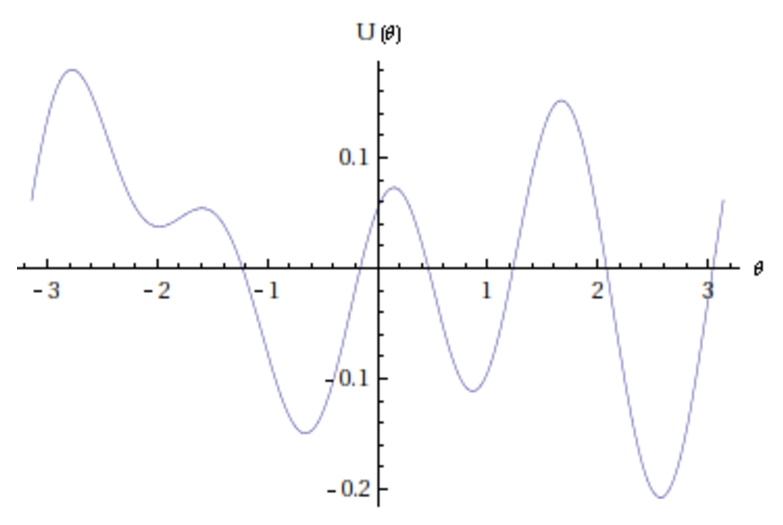
\includegraphics[width=0.45\textwidth]{ks22sliceCond}
 ~~(b)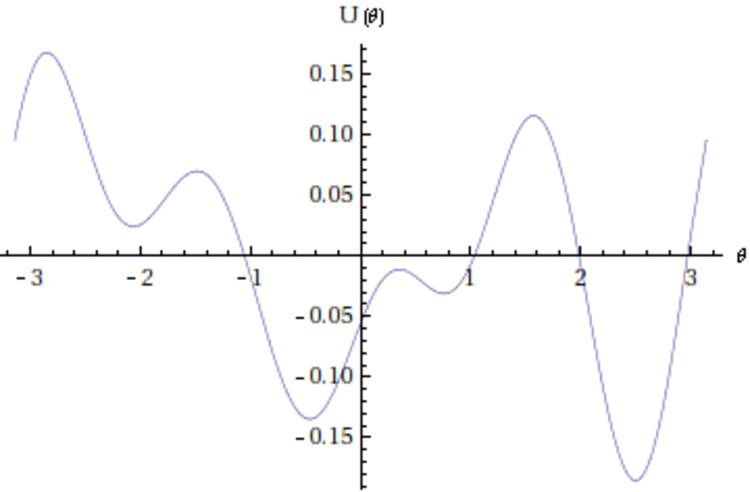
\includegraphics[width=0.45\textwidth]{ks22sliceCond2}
\caption{\label{ks22sliceCond}
Two snapshots of slice fixing condition \refeq{slicFixTW1} along \rpo\
with $\period{p}=16.31,\shift_p=-2.863$.
}
\end{figure}
%%%%%%%%%%%%%%%%%%%%%%%%%%%%%%%%%%%%%%%%%%%%%%%%%%%%%%%%%%%%%%%%%%%%%


What I find remarkable about \reffigs{ks22rpo16mf}{ks22rposMF} is that
I see no $ \dot{\gSpace} \to \pm\infty$ jumps.

%%%%%%%%%%%%%%%%%%%%%%%%%%%%%%%%%%%%%%%%%%%%%%%%%%%%%%%%%%%%%%%%%%%%%
\begin{figure}
 (a)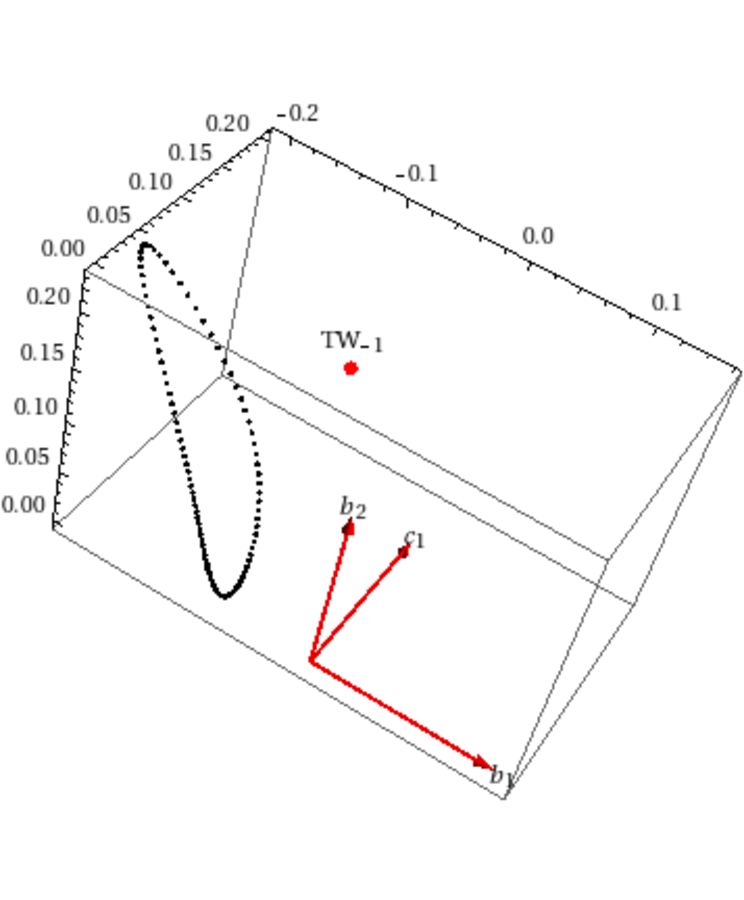
\includegraphics[width=0.45\textwidth]{ks22rpo16mf}
 ~~(b)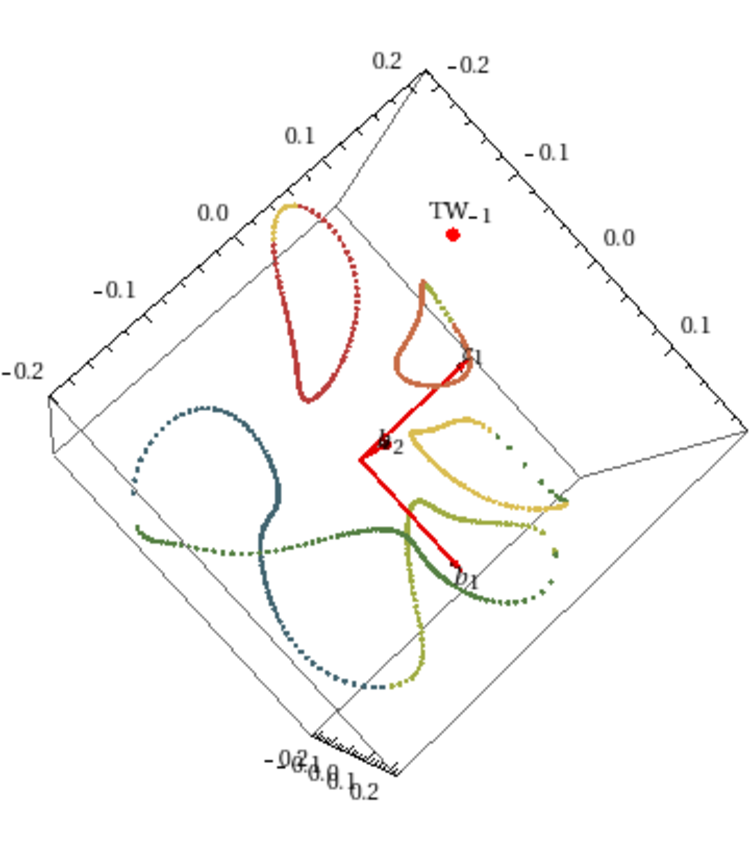
\includegraphics[width=0.45\textwidth]{ks22rpo16mfAll}
\caption{\label{ks22rpo16mf}
\Rpo\ with $\period{p}=16.31,\shift_p=-2.863$ on the \refeq{slicFixTW1} slice.
(a) Tracking solution that corresponds to $\theta$ that maps
$x_p(0)$ to a point of minimum distance from
$\ssp_{TW_{-1}}$,
(b) Accept all $\theta$ and plot all corresponding points.
Color-coding represents internal numbering of solutions and
changes along orbits when the number of solutions for
$\theta$ changes. Note that we have $3$ closed-loop images of
the rpo and $3$ images that appear to connect to a closed
loop. It appears there might be a discrete symmetry here but
I haven't been able to show this.
}
\end{figure}
%%%%%%%%%%%%%%%%%%%%%%%%%%%%%%%%%%%%%%%%%%%%%%%%%%%%%%%%%%%%%%%%%%%%%

%%%%%%%%%%%%%%%%%%%%%%%%%%%%%%%%%%%%%%%%%%%%%%%%%%%%%%%%%%%%%%%%%%%%%
\FIG{
 (a)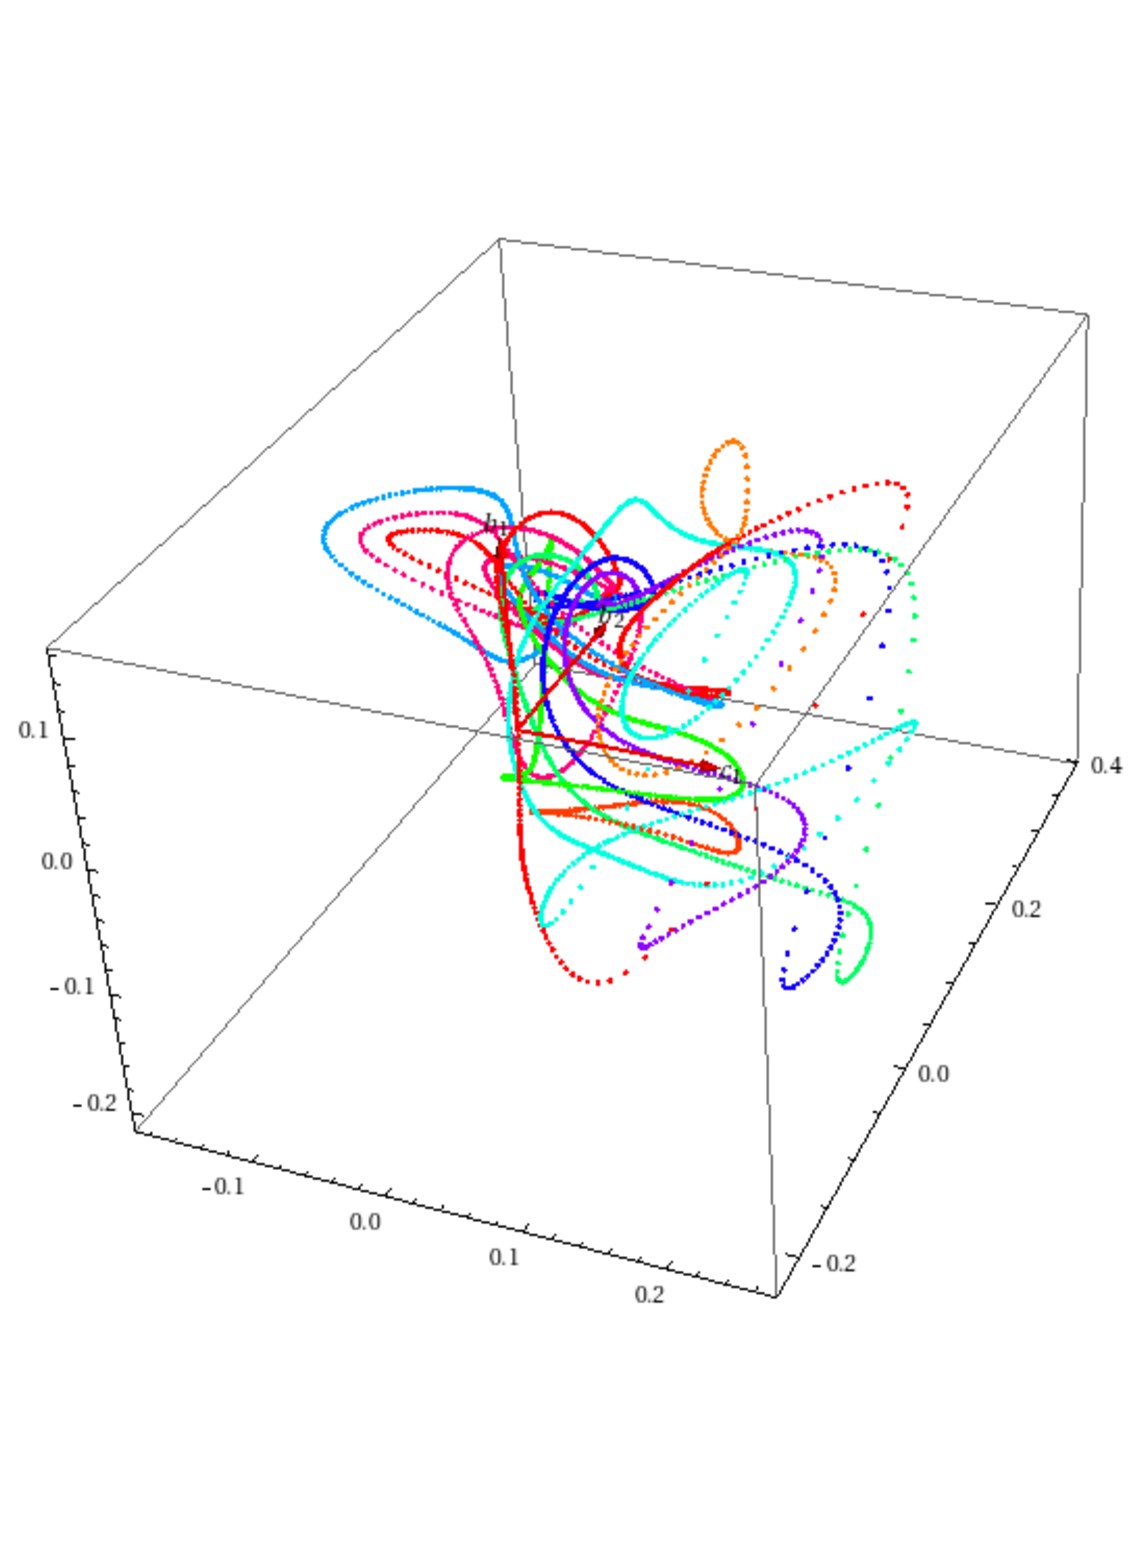
\includegraphics[width=0.45\textwidth]{ks22rposMF}
 ~~(b)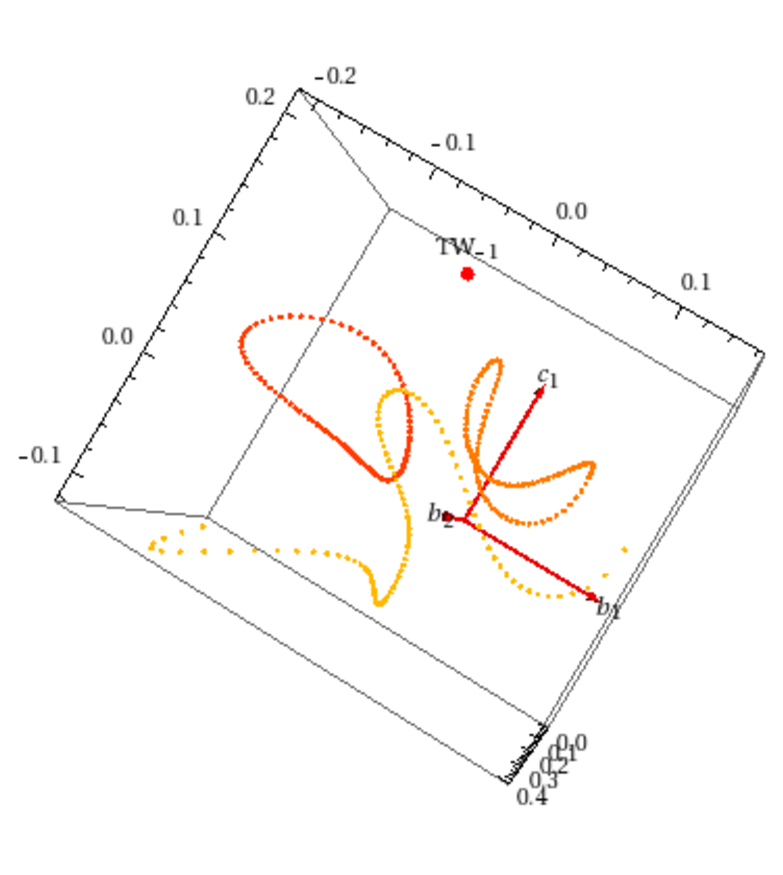
\includegraphics[width=0.45\textwidth]{ks22mf3rpo}
 }{}{
(a) Sample \rpo s and \po s that appear as closed loops after
symmetry reduction through a moving frame that maps them on
on the \refeq{slicFixTW1} slice.
(b)  \Rpo\ with $\period{p}=16.31,\, \shift_p=-2.863$ and \po\ with
$\period{p}=20.51$ appear as closed loops on the slice. \Rpo\ with
$\period{p}=32.80,\, \shift=10.958$ does not appear closed when mapped
back to the slice (the branch that is at minimum distance
from $\ssp_{TW_{-1}}$). We could still have a closed loop
solution but tracking the branches is something I will leave
for later.
}{ks22rposMF}
%%%%%%%%%%%%%%%%%%%%%%%%%%%%%%%%%%%%%%%%%%%%%%%%%%%%%%%%%%%%%%%%%%%%%

\item[2010-01-04 Evangelos]
The good news is that using a traveling wave to
fix a slice was sufficient to reduce about 40\%\ of the short orbits I've
tested to closed loops. For the rest we need a different slice.

\item[2010-01-05 Predrag] Do not understand. Are you saying that the
60\%\ of the short orbits you have tried do not close after one relative period,
or that they encounter the $ \dot{\gSpace} \to \pm\infty$ jumps?

\item[2010-01-05 Evangelos] Sorry, I was not clear on this. 60\%\ of the short orbits
I have tried do not close after one relative period. Since I just use the finite
transformations version (the ``moving frame method'') I do not need to worry about
$ \dot{\gSpace} \to \pm\infty$ jumps. There is some stretching of some orbits even the
ones that are closed loops after reduction, but it is not a great concern.

I wonder whether method of slices (integration on the slice) and moving
frame method (post-processing approach followed here) fail at the same
points. In theory the latter should only fail at points left invariant
under a continuous subgroup, for KS only at the origin. In practice where
a moving frame fails also depends on the choice of slice as we have seen
in \cLe.

\item[2010-01-05 Predrag] If the dot product of slice tangent
and orbit tangent are dominated by 3rd Fourier mode, \rpo\
will close only after 3rd repeat, so run them for several
periods.

\Mslices\ and \mframes\ `fail' at the same point, where the
denominator in the reconstruction equation goes through zero.
They do not fail, they just have a $\pi$ jump there.

Why do you guys keep saying that the \mslices\ fails for the
\Fix{\Group}\ flow-invariant subspace? The subspace is within
the slice. $\dot{\gSpace}=0$, the slice velocity equals the
full space velocity, so there is no problem, methinks.

\end{description}

\section{2010-01-07 Blogging on}

\begin{description}
\item[2010-01-07 Predrag]
Erik Bollt says that your methods of iteratively refining
symbolic dynamics from periodic orbits might work for KS
orbits. I cannot see how he would do it for RPOs (Euclidean
distance is used), but maybe he can get some symbolic
dynamics from the pre-periodic 20,000 orbits?

\item[2010-01-08 Ruslan]
The problem with this approach is that one has to have a
rough idea of the partition to start with, so it can then be
refined using longer orbits.  It worked well for Henon and
Ikeda, but couldn't cope with more complicated 2-dim maps,
e.g. Ueda attractor, having 5-6 fixed points and needing at
least as many symbols).

A while ago I did some work along similar lines when I looked
at the 'proximity' of chaotic orbits to RPOs.  This piece was
not included in our paper, but it must be floating somewhere
(see, e.g., my talk
/siminos/rpo\_ks/davidchack/GaTech030507.ppt).

This is an empirical approach based essentially on a
combination of pattern recognition and time series analysis:
pieces of orbits that look similar (i.e. are close to each
other in phase space in any appropriate metric) can be
labeled by the same 'symbol'.  Then we can try to construct
a transition matrix between symbols based on the observations
of which patterns follow which.  If we manage to do this for
periodic orbits (both RPOs and PPOs) we may be able to get a
rough idea of the dynamical structure of the system.
There is no problem with symmetries here, since we can define
a metric by minimizing the distance with respect to shift and
reflection.

If what I'm doing now fails, I may get back to this idea.

\item[2010-01-05 Evangelos]
Gr\"obner basis $\neq$ Hilbert basis.

\item[2010-01-07 Predrag] Splitting hairs?:
\\\-
\HREF{http://en.wikipedia.org/wiki/Hilbert\%27s_basis_theorem}
{en.wikipedia.org/wiki/Hilbert's basis theorem}:
Hilbert method does not give an algorithm
to produce the finitely many basis polynomials for a given
ideal: it only shows that they must exist. One can determine
basis polynomials using the method of Gr\"obner bases.
{\bf ES} Yes, but why not?

\item[2012-02-27 Predrag]
A reference I have not checked: Guyard\rf{Guyard99},
\emph{Gr\"obner bases, invariant theory and equivariant dynamics}. He writes:``
This paper is about algorithmic invariant theory as it is required within
equivariant dynamical systems. The question of generic bifurcation
equations (arbitrary equivariant polynomial vector) requires the
knowledge of fundamental invariants and equivariants. We discuss
computations which are related to this for finite groups and semi-simple
Lie groups. We consider questions such as the completeness of invariants
and equivariants. Efficient computations are gained by the Hilbert series
driven Buchberger algorithm because computation of elimination ideals is
heavily required. Applications such as orbit space reduction are
presented.
''

\item[2010-01-23 Evangelos]
Written out with pen and paper slice condition for cLe
explicitly and found $\theta$ as a function of
$\theta(\ssp)$. Then cross-checked with
testing/flows/CLEfinalTmp.nb and realized I could also
determine the singular subspace and show that slices and
moving frames are singular at the same points. Then I could
visualize the subspaces and get insight on how to perturb the
slice fixing point so that trajectories do not reach the
singularity. Not sure if this will help with KS, though.
Anyway, I've spend half a day on this but thankfully it is
simple enough to be included in the paper, at least
partially, making the paper a bit thicker in formulas.


\item[2010-01-23 Evangelos]
Using EventLocator testing/flows/CLEfinal.nb I checked that
integration on the slice for CLe approaches but does not
reach singularity.

\item[2010-01-28 Evangelos Siminos]
The last chapter of volume two of Byron and Fuller\rf{ByFu92}
{\em Mathematics of Classical and Quantum
Physics}
is an introduction to
group theory even more compact than Tinkham's first chapters. Worth to
have a look just for this. Georgia Tech has it.
According
to Byron and Fuller, which I find a very reliable and carefully written
book, what I use right now is the convention most physicists
use for \emph{active} transformations. This I've also used
in thesis and I'd be happy to stick with this. With this choice
small angle, active rotations, are counterclockwise, so I've updated
our orientation condition as well.
\\
{\bf PC 2010-12-12~} Thanks, let's make sure that we have the
right sign in discrete.tex, continuous.tex.
Never seen Byron and Fuller, still.

\item[2010-02-02 Predrag]
The holidays are over. ``That integration on the slice for
CLe approaches but does not reach singularity'' worries me. I
would feel better if you checked the crossing by the method
of moving frames, \ie, integrate the full system and keep the
sign relative to the 3-dim subspace. I suspect it crosses,
but if we integrate in the slice the integrator fights against it,
keeps the \reducedsp\ trajectory on one side of the $\infty$- reduced
velocity abyss.

\item[2010-02-03 Evangelos]
Actually I've checked it using moving frames before checking using slices.
I was afraid that in moving frames I just sample points that have the same
sign and miss crossings of the singularity. No, both methods show the same.
One more thought is that I should try is to switch to a more brutal integrator,
see how it behaves.

The way I see it is that with the general linear slice,
together with the orientation condition we introduce some
sort of generalized polar radius that cannot become less than
zero. In contrast if we do not impose the orientation
condition we really get into trouble: both me and Halcrow
tried that with ZM and I think what we got was real
discontinuities in the flow. Rebecca also had this problem in
exercise 2.19 of her blog, where she used $\cos(\theta)$ to
define the moving frame. This is not shown in her figure 2.1,
as she only plots her trajectory for $t$ up to $50$. I've
proposed to her to integrate up to $t=200$ and see what
happens but she did not do it. What you will see is a
two-eared attractor with instant transitions between ears in
certain projections. Anyway, this is all post-processing. I
do not really understand why, but in the method of slices
orientation condition is satisfied without us enforcing it.
So, what I mean by saying we do not have a problem with CLE
and the method of slices, is not that there is no
singularity, but that we stay on one side of it.

\item[2010-02-03 Evangelos] I will run some more tests but I am kind
of fed up with CLe, I want to go back to the real thing and try
to get it to work with KS.

\item[2010-03-04 Predrag]
Kevin Mitchell is here, says we should study Littlejohn and
M. Reinsch\rf{LiRe97}: ``Gauge fields in the separation of
rotations and internal motions in the $n$-body problem.'' I
will put it into \wwwcb{/library}. Read 3-body problem
sections. See p. 14 for a discussion of the three-body
coordinates and p. 25 for a discussion of the three-body
section (gauge).

\item[2010-03-08 Predrag]
``Connecting curves for dynamical systems'' by
R. Gilmore, Jean-Marc Ginoux, Timothy Jones, C. Letellier, and U. S.
 Freitas\rf{GGJLF10} looks interesting. They say:
``
 We introduce one dimensional sets to help describe and constrain the integral
curves of an $n$ dimensional dynamical system. These curves provide more
information about the system than the zero-dimensional sets (fixed points) do.
In fact, these curves pass through the fixed points. Connecting curves are
introduced using two different but equivalent definitions, one from dynamical
systems theory, the other from differential geometry. We describe how to
compute these curves and illustrate their properties by showing the connecting
curves for a number of dynamical systems.
''


\item[2010-03-30 Predrag] This entry should probably be moved
to lippolis/blog, but as it is about adding noise to PDEs we might need it for
`optimal partitions' of PDEs such as \KSe\ and \NSe.
Went to
Stochastics Seminar to hear
Boris Rozovsky (Applied Math, Brown), joint work with
R. Mikulevicius, talk about
``Quantization of Stochastic Navier-Stokes Equation.''
They say:

`` We consider a stochastic Navier-Stokes equation driven by a space-time
Wiener process. The equation is ``quantized'' in the Paris-Wu
sense by transformation of the
nonlinear term to the Wick product form. An interesting feature of
this type of perturbation is that it preserves the mean dynamics: the
expectation of the solution of the quantized Navier-Stokes equation
solves the underlying deterministic Navier-Stokes equation (\ie,
the leading term in the weak-noise expansion is the classical solution).
From the
stand point of a statistician it means that the perturbed model is
an unbiased random perturbation of the deterministic Navier-Stokes
equation. The quantized equation is solved in the space of generalized
stochastic processes using the Cameron-Martin version of the Wiener
chaos expansion. A solution of the quantized Navier-Stokes equation turns out
to be non-anticipating and Markov.

\item[2010-03-31 Evangelos] Robert Gilmore on CLe paper (2010-03-18):\\

As you write ''....it's a very tough problem.''\\

There is not much I can add to what you have written,
except to say that the problem of locating the components
of the Poincar\'e surface of section is somewhat
under control for dissipative flows in $R^3$.
I wonder what the generalization looks like in
higher dimensions.


\item[2010-05-13  Evangelos]

Mahmoud, Bountis \etal\rf{mahmoud09} study ZM, Mahmoud
\etal\rf{mahmoud08a} study CLE. Nothing of interest for CLE paper. From
Mahmoud \etal\rf{mahmoud08b} I've only learned there is an Egypt-Greece
Scientific and Technological cooperation. We can cite these papers to
show there is recent interest on CLe, but on the other hand I don't see
relation to what we do.
\\
{\bf Predrag:} let's ignore them.

Fowler and McGuiness\rf{FoMcGui84} study bifurcations of CLe relative equilibrium
to relative periodic orbits (I'll cite it).

Roekaerts, Flessas and Leach\rf{Ro88,Fl89,FlLe91} show integrability
and find particular solutions of CLE for specific parameter values.
Too parameter-specific to be of use to us.


\item[2010-06-15 Predrag] Just talked to
\HREF{http://www.crcg.de/wiki/Chenchang_Zhu}
{Chenchang Zhu}. The name has to be sung, with high note on `Zhu.'
She probably knows much more than we would ever wish to know;
was on Chinese team in a Math Olympiad, Weinsten's Ph.D. at Berkley.
Bad news: Grothendick thought about it deeply, and said
													\toCB
 - ``why
symmetry reduce? The result is invariably ugly. Let's keep everything
the way it is, and describe it in terms of categories.'' Not kidding.

\item[2010-10-11 Gelfert and Motter] say in
\HREF{http://arxiv.org/abs/1010.1791} {(Non)Invariance}  of dynamical
quantities for orbit equivalent flows: `` We study how dynamical
quantities such as Lyapunov exponents, metric entropy, topological
pressure, recurrence rates, and dimension-like characteristics change
under a time reparameterization of a dynamical system. These quantities
are shown to either remain invariant, transform according to a
multiplicative factor or transform through a convoluted dependence that
may take the form of an integral over the initial local values. We
discuss the significance of these results for the apparent non-invariance
of chaos in general relativity and explore applications to the
synchronization of equilibrium states and the elimination of expansions.
''

The paper is written by
\HREF{http://arxiv.org/find/math/1/au:+Gelfert_K/0/1/0/all/0/1}
{Katrin Gelfert} (a mathematician from Rio) and therefore essentially unreadable.
 Cycle expansions are the primitive kinds mathematicians tend to use:
``By a well-known result on the equidistribution of closed orbits for blah
we know that the unique equilibrium state blah blah with respect to blah
is obtained as the weak limit of the weighted orbital measures.''
(irrelevant math reference) etc., etc.. Still, it might be worth a read, as
general relativity is one of the things to think about in the
turbulent years ahead.

She has also written on
\HREF{http://arxiv.org/abs/0901.2139}
{On the distribution of periodic orbits}, a similarly cheerful reading
which again does not refer to you-know-who. Life in separate universes.

Will keep you posted.

\item[2010-11-12 ES] You might also want to have a look at \cite{motter09},
written by Motter, more readable.

\item[2010-11-18 Predrag talked to Sandstede]
He agrees that Hilbert polynomials are not an option for higher dimensions,
the only thing that works is slicing. He does not what to make out
of the "method of connections" either. He cannot read Marsden either.
In their papers they have to increase the
space in (to me non-obvious manner) because they are studying
bifurcations of equilibria with nontrivial symmetry, so slice cannot be
defined the way we define it, as a hyperplane normal to the group tangent
space - that one has lower dimension than the group.

They used the same linear slice condition that we do, but being mathematicians,
they did not need to invert any matrices to get an explicit equation for
$\dot{\gSpace}$; for them it sufficed to know that it can be done.
He thinks the answer for compact Lie symmetry groups is in Krupa, but
we did not find out where. If it is there at all. He promised to find out
from his notes and let me know what the formula is.

\item[2010-11-19 Evangelos]
Any good idea now on how to quotient KS?

\item[2010-11-20 Ruslan]
Not really.  I still believe that our best bet for quotienting \On{2}
symmetry from functions defined on a circle is to fix the phases of
Fourier modes (hierarchically).  The problem is to link slices defined
for different modes in a way that is natural for the KS dynamics.  As I
described some time ago in this blog, one of the problems I was struggling
with was to link in a natural way the dynamics within the antisymmetric
subspace with that in the full space.  I still don't see a neat way
forward, but frankly I didn't have a chance to spend much time thinking
about it.  It would be nice to have somebody like Stefan, who could try
out a few ideas and see where they take us, since I cannot find enough
time to do it myself.  I'm currently looking for a student (undergrad or
PhD) who's good enough to take up this project.


\item[2010-11-20 Predrag]
\texttt{[2010-12-15 PC: incorporated this entry into}
 \texttt{frehlich slice article]}
\\
Looks like we are digging into positions which are essentially aesthetic
- we agree on the need for a set of slices, but not on a criterion on
how to pick them. Ruslan's proposal is purely group theoretic: pick a slice
within a symmetry subspace $C_k \in \SOn{2}$, pick the next one when this
fails you. I'm guided by \KS\ work with Lan, where \Poincare\ sections
are picked physically,
by neighborhoods of important solutions (2-rolls states, 3-rolls
states). The choice should be `physical,'
dictated by the dominant patterns seen in the solutions of
nonlinear PDEs.
I'll write up the proposal that follows
in the paper with Stefan\rf{FrCv11}.

Even though every generic
slice cuts all group orbits, it makes no sense physically to
use one slice
(a set of all group orbit points that are closest to a given `template')
globally. Instead we should do what we
already do for \KS\ Poincar\'e sections. While \refref{Christiansen97} demonstrated
that \po\ theory can be applied to spatially extended systems, the
main advance of
\refref{lanCvit07} was to show that for more turbulent/chaotic systems a set
of Poincar\'e sections is needed to capture the dynamics.
A slice defined here is a purely group-theoretic, linear construct, with no reference
to dynamics; a given slice-fixing point (template) \slicep\ defines
the associated slice, a ($d\!-\!N$)-dimensional hyperplane.
Within it, there is a ($d\!-\!N\!-1$)-dimensional
singularity hyperplane
\[
\braket{\groupTan(\sspRed)}{\sliceTan{}}=0
\]
where the group tangent of a point
$\sspRed=\LieEl^{-1} \ssp$ lies in the slice. The singularity hyperplane
is also purely group-theoretical,
determined by the slice-fixing point (template) \slicep,
that pays no heed to nonlinear dynamics. If we pick another
slice-fixing point $\slicep'$, it comes along with its own slice
and singularity hyperplane. So idea is to coarsely cover the nonlinear
strange attractor with a set of hyperplanes, as in \reffig{fig:Tesselate}.
For any pair, they intersect in a 'boundary' hyperplane, of one less dimension.
So our task is to, for a given strange attractor, pick a set of slice-fixing
points, such that each is approximately tangent to the strange attractor,
and the singularity hyperplanes are eliminated by requiring that they
lie either on the `wrong' side of the slice-slice intersection, or somewhere where
the strange attractor does not tread.

We need to make a global chart by deploying both linear slices and linear
Poincar\'e sections in neighborhoods of the most important (relative)
equilibria and/or (relative) periodic orbits (those are tricky, because
slice fixing points must lie in the full \statesp, and have no symmetry,
so most of the solutions we have are not good as they stand). This is the
periodic-orbit generalization of the idea of
% \HREF{http://chaosbook.org/overheads/trace/Tesselate.jpg}
{\statesp\ tessellation}
so dear to professional cyclists, \reffig{fig:Tesselate}.

% In FrCv11.tex replace by Tesselate.png
%%%%%%%%%%%%%%%%%%%%%%%%%%%%%%%%%%%%%%%%%%%%%%%%%%
\SFIG{f_1_08_1}
{}{
Smooth dynamics  (left frame) tesselated by the skeleton of
periodic points, together with their linearized neighborhoods,
(right frame).
Indicated are segments of two 1-cycles and a 2-cycle that
alternates between the neighborhoods of the two 1-cycles,
shadowing first one of the two 1-cycles, and then the other.
}{fig:Tesselate} %{Hyp} %{fig6} and {tr:fig6} in ChaosBook
%
%%%%%%%%%%%%%%%%%%%%%%%%%%%%%%%%%%%%%%%%%%%%%%%%%%
%


Boundaries
between hyperplanes are themselves hyperplanes of one dimension less and
should be easy compute once we have decided on the set of slices. To find
what slice a given full \statesp\ trajectory point is in, one group-rotates
with respect to each slice, and checks whether the given group orbit
belong to it. In the \reducedsp\ the trajectory is integrated within a
given slice until it hits a hyperplane boundary - then one switches to
the next slice across the boundary. This passage does not need to
be computed very precisely, as long as the singularity
hyperplanes are kept a safe distance away. Boundary corners are measure zero, no
way you would hit them.

Global chart should be sufficiently fine-grained that we never hit any
slice singularities. That means that the neighborhood - bounded by
intersections with neighboring slices is sufficiently small that group
tangent space is nowhere within the part of the slice explored by
the strange attractor - works for smooth flows
with sufficiently small neighborhoods.

\item[2010-12-02 PC]
\HREF{http://arxiv.org/abs/1012.0076}{``Un-reduction''}
by Bruveris, Ellis, Gay-Balmaz and Holm\rf{BrEllGBAHo10},
sound provocative. They say: ``
We give a full geometric development of a new technique called
un-reduction, for dealing with dynamics and optimal control problems posed on
spaces that are unwieldy for numerical implementation. The technique, which was
originally conceived for an application to image dynamics, uses Lagrangian
reduction by symmetry in reverse. A deeper understanding of un-reduction leads
to new developments in image matching which serve to illustrate the
mathematical power of the technique.
''

\item[2010-12-06 PC]
\HREF{http://webusers.physics.uiuc.edu/~goldbart/PostScript/MS_PG_book/bookmaster.pdf}
{Stone and Goldbart}\rf{StGo09} Sect 1.5 discussion of Lagrange
multipliers, simple and intuitive, suggests that we should think of
symmetry reduction of dynamics to a slice in terms of Lagrange
multipliers. Perhaps we can finally get a clear exposition that unifies
our discussion of \Poincare\ sections and \reducedsp\ with our methods of
finding \po s and \rpo s, where we increase dimension by one for every
continuous symmetry dimension. Rytis starting writing that up for
ChaosBook (it is in the boy scout edition) but characteristically left in
limbo.

\item[2010-12-04 PC]
As a curiosity, in presence of noise we might want to replace the Euclidean
distance by a variant of the
\HREF{http://en.wikipedia.org/wiki/Mahalanobis_distance}
{Mahalanobis distance}, or something dynamically even
smarter\rf{LipCvi08,LipCvi07}.

\item[2008-09-01 PC] (rescued this from siminos/blog/flotsam.tex
have not read this ever list)
Following might be of interest (have not checked myself):


\noindent
Thomas J. Bridges\rf{Bridges08},
\HREF{http://personal.maths.surrey.ac.uk/st/T.Bridges/PAPERS/JDEQ06-466.pdf}
{\emph{Degenerate relative equilibria,}}
\emph{curvature of the momentum map, and homoclinic bifurcation}

Muriel Koenig,
\HREF{http://journals.cambridge.org/action/displayAbstract?fromPage=online&aid=37117}
{\emph{Linearization of vector fields}}
\emph{ on the orbit space of the action of a compact Lie group}

Pascal Chossat\rf{Choss02},
\HREF{http://www.springerlink.com/content/7wmkx35tqvfekw04/}
{\emph{The reduction of equivariant dynamics}}
\emph{to the orbit space for compact group actions},
{\em Acta Applicandae Mathematicae \bf 70}, 71 (2002). %71-94

\HREF{http://www.ams.org/notices/200503/fea-bloch.pdf}
     {Bloch \etal}\rf{BlMaZe05} say:
``A classical reference for the rolling disk is [German
sociologist]
\HREF{http://alo.uibk.ac.at/webinterface/library/ALO-BOOK_V01?objid=12421&zoom=6}
{Vierkandt}\rf{Vierkandt1892}, who showed
something very interesting: On an appropriate
symmetry-reduced space, namely, the constrained velocity
phase space modulo the action of the group of Euclidean
motions of the plane, all orbits of the system are
periodic.''

This is tedious and hated by all, but sometimes useful:
Arfken and Weber\rf{ArWe05},
\emph{Mathematical Methods for Physicists: A Comprehensive Guide
}
%\HREF{}
%{}


\item[2010-12-13 PC]
This is misplaced, will eventually move to a 'mixing' blog, but:
Maxey and Riley\rf{MaRi83},
{\em Equation of motion for a small rigid sphere in a nonuniform flow}
seems important in $2D$ mixing - Golub uses it.

\item[2010-12-28 PC:
{\PoincSec}s from the closest recurrences]
A false epiphany; what we do for slice, does not quite works for linear
{\PoincSec}s.
The problem is that we lack a definition of distance
between points on different trajectories that is invariant under time
evolution (details scribbled in United Airlines flight 941, still to be
written down here). Gibson's \pCf\ Poincar\'e section in terms of
equality of dissipation and boundary shear is a step in right direction;
perhaps.

Shift in time to the closest passage\rf{pchaot,MFKM10,CviGib10} is what we
call a
`close recurrence.' Perhaps this is related to the ``problem of recognition''
described in Golubitsky and D. G. Schaeffer\rf{golubI}, a much more
ambitious scheme of local nonlinear mappings that take an \eqv\ into
something as close as possible to a {\template} / `normal form.'

\item[2010-12-28 PC]
\HREF{http://arxiv.org/abs/1012.5060}
{``Invariant higher-order variational problems''}
by Gay-Balmaz, Holm, Meier,  Ratiu, and Vialard\rf{GBHMRV10}. They say: ``
We investigate higher-order geometric $k$-splines for template matching
on Lie groups. This is motivated by the need to apply diffeomorphic
template matching to a series of images, e.g., in longitudinal studies of
Computational Anatomy. Our approach formulates Euler-Poincar\'e theory in
higher-order tangent spaces on Lie groups. In particular, we develop the
Euler-Poincar\'e formalism for higher-order variational problems that are
invariant under Lie group transformations. The theory is then applied to
higher-order template matching and the corresponding curves on the Lie
group of transformations are shown to satisfy higher-order
Euler-Poincar\'{e} equations. The example of SO(3) for template matching
on the sphere is presented explicitly. Various cotangent bundle momentum
maps emerge naturally that help organize the formulas. [...].
''

The usual tough ploughing. They say the basic reference is \refref{HMR98}.
I do not understand even the zeroth step, \ie, can any of this be used for
flows which are not Lagragian/Hamiltonian? Seems not.

\item[2011-01-15 PC] writes in the slice paper,
\HREF{http://www.cns.gatech.edu/~predrag/papers/preprints.html\#FrCv11}
{\emph{Reduction of continuous symmetries}} \emph{of chaotic flows by the
method of slices}

Two
hyperplanes are associated with  any given {\template} \slicep; the slice,
%\refeq{PCsectQ},
and the hyperplane of points \sspSing\ such that from
the {\template} vantage point their group orbits are not transverse, but
locally `horizontal,'
\beq
\braket{\groupTan(\sspSing)}{\sliceTan{}}
 =
\braket{\sspSing}{\Lg^2\slicep}
 =0
%\,.
\ee{sliceSingl0}
(for simplicity, in this section we specialize to the  $\SOn{2}$ case).
We shall refer to the $(d\!-\!2)$\dmn\ intersection of the two as the
{\em \sset} $S$,
\beq
\braket{\groupTan(\sspRSing)}{\sliceTan{}}
 =
\braket{\sspRSing}{\Lg^2\slicep}
 =0
\,.
\ee{sliceSingl}


\item[2011-01-15 PC] writes slice article: ``
In \refref{SCD07} it
was found that the coexistence of four \eqva, two \reqva\
(traveling waves) and a
nested \fixedsp\ structure in an effectively $8$-dimensional \KS\ system
complicates matters sufficiently that no symmetry reduction has been
attempted so far.
''

\item[2011-01-15 ES]  Not attempted? Not funny. You seem to
totally forget my thesis, but I have to say that not only it attempted
but also succeeded to provide global invariant coordinates, analytically
and in $128$ dimensions. You might not like it for aesthetical reasons,
but you cannot say it was not attempted -- it was an effort of
at least three years involving me, Ruslan, Predrag, Jonathan (and I might
forget someone).

\item[2011-01-15 PC]
OK, I'll fess up and confess: I HAVE read the
\emph{\HREF{http://www.chaosbook.org/projects/Siminos/thesis.pdf}
           {Thesis that Nobody Reads}}.
I would not stick my hand in fire that Stefan has done it, but he's
operating under the undergraduate exclusion clause. And my wife is right
when she says I'm a brute, I meant to `not attempted by the \mslices' as
outlined in the slice paper. Sorry. Rewritten now.

\item[2011-01-13 SF]
For the nearby trajectories the numerator is nonzero, but along a
trajectory passing through a singularity doesn't the numerator approach
zero $\gSpace$ approach the angle required to rotate the velocity into
the slice? Hence the infinitely thin delta function. {\bf ES} I am also
confused about what happens in the last two paragraphs, but I'll let you
two sort it out first.

\item[2011-01-14 PC] I have discussed this with Stefan, and I think he
was confusing \mframes\ (where you have a freedom to rotate $\ssp$ (and
$\vel(\ssp$ with it) with \mslices, where symmetry reduction has already
taken place, $\sspRed$ cannot be rotated, and $\vel(\sspRed)$ is the
\emph{full} \statesp\ velocity which points wherever it pleases, even
though it is evaluated on a slice point $\sspRed$, so
${\braket{\vel(\sspRed)}{\sliceTan{}}}$ generically does not vanish.


\item[2011-01-15 PC] In the slice paper I make a bold claim:
``While all group orbits of a  generic trajectory cross the slice, the
trajectory has vanishing probability to cross the lower-dimensional
{\sset} - that is why we had to `engineer' the slice in [our \cLe\ example].
However, an ergodic trajectory  might come arbitrarily close to  $S$
arbitrarily often.''

This hopefully resolves a long-standing conundrum for Evangelos and me.
Please CORRECT ME if I am wrong, I'm on thin ice here!


%%%%%%%%%%%%%%%%%%%%%%%%%%%%%%%%%%%%%%%%%%%%%%%%%%%%%%%%%%%%%%%%%%%%%%%%

\item[2011-01-17 Ashley]
The draft reads pretty well to me.  There were a couple of bits I don't
get but can discuss later - I've tried tessellating using all the known
states in our 2.5D m=2 pipe.  Intermediate success.  Will post on the
blog presently.

\begin{enumerate}
  \item The use of 'template' in the abstract threw me a bit.  Is there
  space to add ", or 'reference state'," for us dummies?
    \\
  {\bf 2011-01-17 PC} I like it, but where did you get
  the term 'reference state' from? I  can find it only under computer science
  literature, have decided to use 'template'  because (a) that's well
  established Marsdenite lingo\rf{rowley_reduction_2003},
  (b) it's very descriptive of what we actually do, and it nicely
  expresses my personal quest for developing a `language of patterns,'
  of which plumbing is but one manifestations (electricians'
  cardiac dynamics labors would be another). We already
  accommodate the dummies the
  first time we define the `template' in the body of the paper:
  ``Think of the first pattern
(represented by a point {\slicep} in the \statesp\  \pS) as a
`template'\rf{rowley_reconstruction_2000,rowley_reduction_2003} or a
`reference state.'~''
In the file, `template' is a macro, it could be easily changed.

  \item Would be good to make more connections with Figure 1 in the
  discussion.  I didn't find a reference to Fig 1(b).
    \\
  {\bf 2011-01-17 PC} Will do. We refer to it once: ``
The first
equation defines the flow confined to the slice (see
Fig. 1\,(b)), '' but now we also refer to it in the introduction.

  \item We seemed to be talking about a single reference state until
  section 3, so in section 2 the last paragraph on p3 about the span of
  several tangent vectors confused me a bit - I thought we were talking
  about the new method before we really were. $\to$ defer to start section
  3(?)
    \\
  {\bf 2011-01-17 PC} cannot find the text you are referring to. In any case,
  the discussion is for any group \Group, so the group tangent space for a
  \emph{single slice} is $N$-dimensional.

  \item Because of the last point, at the top of p5 when we 'pick the
  closest' I wasn't sure if you we already including the closest to any
  reference state already, but it looks like just the closest minimum
  from for one state.  The Newton method reducing the work at this point
  doesn't seem entirely satisfactory, and it would not detect new minima
  arising and possibly getting closer later on (which would also cause a
  jump).
    \\
  {\bf 2011-01-17 PC}
You are right, I have now added a paragraph discussing the point you rise
here.
    \\
  {\bf 2011-01-19 ES}
This remark reminded me that I had tried using Newton's method with
a guess from the previous point to get the solution on the slice
that is at minimum distance from the template, in order
to get \reffig{ks22rpo16mf}. However, there were problems with jumps,
as correctly pointed by Ashley. So I've ended up finding all solutions
and picking the one which was at a minimum distance from the template.

  \item In section 4 it wasn't obvious to me what was meant by {\em linear slices}.
    \\
  {\bf 2011-01-17 PC} You are right: all our slices are linear.
  Now removed/edited.

  \item Minor style difference (UK-USA difference?) - I use commas only
  in lists of nouns, and for other lists hyphenate where necessary e.g.
  "spatially-extended turbulent flows".  I've only mentioned it as it
  occurs in the first sentence of the Intro.
    \\
  {\bf 2011-01-17 PC}
I now made it `spatially-extended' throughout, no doubt introducing
new stylistic boo-boos. Or boo boos.

  \item An open issue that came up for me (can repost on blog), and
  appears to be alluded to at the end of section 4, is how to pick the
  shift of the reference states.  Any ideas?
    \\
  {\bf 2011-01-17 PC}
You are right, this is THE question.
The first one is for free, but that, I believe, fixes then all relative
phases to the succeeding {\template s}. It is more than alluded to:
``
There is a rub, though - you need to pick the phases of neighboring
{\template s} in such way that you minimize the distance from one to the
next as the ant crosses the ridge. This a reflection of the flaw inherent in use
of a linear, hyperplane slice globally: a slice is derived from the Euclidean
notion of distance, but for nonlinear flows the distance has to be
measured curvilinearly, along unstable
manifolds\rf{Christiansen97,DasBuch}. We nevertheless have
to stick with tessellation by
linearized tangent spaces, as curvilinear charts seem computationally too
prohibitive. The {\em relative phase} between two
different \reqva\ can be fixed, as proposed in \refref{SCD07}, by the
shortest heteroclinic connection, a rigid bridge from one
neighborhood to the next.
''

In the abstract of \refref{SCD07} we say
``We show,
on the example of a particular small-cell Kuramoto-Sivashinsky
system, how the geometry of its dynamical state space is
organized by a rigid `cage' built by heteroclinic connections
between equilibria, [...]'' and then in the body of the paper:

``
The main results presented here are: [...] (b)
Existence of a rigid `cage' built by heteroclinic connections
between \eqva.
''

``
Here we demonstrate that, for \rpo s visiting the
neighborhood of equilibria, if one picks any
particular solution, the universe of all other solutions is rigidly
fixed through a web of heteroclinic connections between them. This
insight garnered from study of a 1-dimensional \KS\ PDE is more
remarkable still when applied to the plane Couette flow\rf{GHCW07},
with 3-$d$ velocity fields and two translational symmetries.
''

Now, whether we have really demonstrated it is in the eye of beholder...


\end{enumerate}

\item[2011-01-17 Ashley]
 How should I pick the shift of the reference states?
 Should I repeat adding, say, 100 randomly chosen turbulent states as reference states?

\item[2011-01-17 PC]  No - as few slices as possible. We just need
to make sure that the ridges between them are sufficiently close
to each the templates template so that the inflection hyperplanes
are excluded. Once templates are picked, the rest is geometry of
hyperplanes (NOTHING to do with dynamics, only with the group theory)
so I think checking whether the inflection hyperplane is on
the far side of the tile edge (ridge between two slices)
is a linear computation, to be undertaken independently of dynamics. I hope...


\item[2011-01-17 PC] Ashley made me do it: I Googled [symmetry reduction
"reference state"]. There is whole new infinite regressions chain of
literature in computer science\rf{Donaldson09c}. Hopefully we can ignore
this - it is about symmetries of data sets under permutations. But the
mathematical language is the same, except that the meaning of 'reference
state' is something that will stop any dummy dead in her tracks.

On the bright side,
a black-headed woman make a freight train
\HREF{http://www.traditionalmusic.co.uk/folk-song-lyrics/Saint_Louis_Blues.htm}
{jump the track},
(but a long tall gall makes a preacher ball the jack).


  \item[Predrag 2010-01-20] See, somebody does check what's on arXiv.
\HREF{http://www.youtube.com/watch?v=BsVxmk9pq2Y}{Marlon Brando}
himself (AKA Krzysztof Kowalski, kowalski@uni.lodz.pl)
writes:

It seems to me
that you would find interesting my joint paper\rf{KoRe96,KoRe98},
``Groups and nonlinear
dynamical systems. Chaotic dynamics on the SU(2)xSU(2) group,''
which is also devoted to the study of continuous symmetries
of chaotic flows.  I attach a copy of this article.
[Predrag uploaded the two articles to Zotero.
\HREF{http://arxiv.org/abs/chao-dyn/9801020}{arXiv:chao-dyn/9801019} and
\HREF{http://arxiv.org/abs/chao-dyn/9801020}{arXiv:chao-dyn/9801020} exist,
but useless - no figures (?!).]

Abstract\rf{KoRe96}: ``
An abstract Newton-like equation on a general Lie algebra is introduced
such that orbits of the Lie-group action are attracting set. This
equation generates the nonlinear dynamical system satisfied by the group
parameters having an attractor coinciding with the orbit. The periodic
solutions of the abstract equation on a Lie algebra are discussed. The
particular case of the SU(2) group is investigated. The resulting
nonlinear second-order dynamical system in $R^3$ as well as its
constrained version referring to the generalized spherical pendulum are
shown to exhibit global Hopf bifurcation.
''

Abstract\rf{KoRe98}: ``
In our previous paper\rf{KoRe96}, we introduced an abstract Newton-like
equation on a general Lie algebra such that submanifolds fixed by the
second-order Casimir operator are attracting set. The corresponding group
parameters satisfy the nonlinear dynamical system having an attractor
coinciding with the submanifold. In this work we discuss the case with
the $SU(2)\times SU(2)$ group. The resulting second-order system in $R^6$
is demonstrated to exhibit chaotic behaviour.
''
Out there in the left field: this Kowalski article\rf{Kowa97}
looks provocative.


\item[2011-04-11 Predrag]
													\toCB
Divakar Viswanath gave us a talk about predictability from
time series (the paper is on his home page). After blah-blah
and the scholarly Shannon information incantations, it gets
interesting: numerous previous prediction schemes (as well as
reduction schemes) were poor predictors because one tried to fit
a (Lyapunov-time comparable) sequences {\em preceding} the window
of prediction. Instead Divakar minimizes the distance to the
state immediately preceding the prediction window; the history
coming up to the present instant might look wildly different, but
the prediction approaches the optimal. The reason is that all
one needs to do is to be close to the stable manifold of the
recent past, not the states themselves.

This should be emphasized in the programmatic parts of ChaosBook,
both the optimal prediction from deterministic data, and in the
noise reduction and control; one needs to get to the stable manifold
ridge of a saddle, that is much more efficient in terms of both control
and the size of the target, than aiming for a desired state itself.

\item[2011-05-06 Predrag] Still bogged down in \refsect{sect:toCB}
and \refexam{exmp:SymplDistance} (``How far are two points from each other
in a symplectic vector space?''), but it got me to thinking about
how far are two solutions in a more general, temporal setting. Smart thing
about Stefan Froehlich's and my symmetry reduction is that instead of
running the full group trajectory to determine near \statesp\ points, we
write an extremal condition for them. In initializing
the \po\ searches by near recurrences in long-time \statesp\
trajectories, we run entire trajectory against it's time delayed version.

\textbf{Question:} Can we instead {\bf define}
the pairwise near recurrences by an extremal
condition? So, instead of running blindly long trajectories, we would
be solving some algebraic condition that singles out extremal points
along the trajectory.

\item[2011-05-18  Rich Kerswell] Read
Irene Moroz,
Geophys. Astrophy Fluid Dynamics vol 105, 273-286, 2011,
\emph{Unstable periodic orbits in 4D Faraday disk dynamo}.
Might give you a 4-dimensional dynamical system which is
chaotic and can be reduced to a 3\dmn\ \statesp; easier to
visualize than {\cLf}.

\item[2011-05-29 Predrag]
\HREF{http://arxiv.org/abs/1105.4180}
{``Phase space structures} governing reaction dynamics in rotating molecules''
by Unver Ciftci and Holger Waalkens is a paper that we (Kamor, Chandre,
Uzer, ...) should study. In particular, Chao, can you alert Adam about
it? They say:

``
Recently the phase space structures governing reaction dynamics in
Hamiltonian systems have been identified and algorithms for their
explicit construction have been developed. These phase space structures
are induced by saddle type equilibrium points which are characteristic
for reaction type dynamics. Their construction is based on a
Poincar{\'e}-Birkhoff normal form. Using tools from the geometric theory
of Hamiltonian systems and their reduction we show in this paper how the
construction of these phase space structures can be generalized to the
case of the relative equilibria of a \emph{rotational symmetry reduced
$N$-body system}. As rotations almost always play an important role in
the reaction dynamics of molecules the approach presented in this paper
is of great relevance for applications.
''

As far as I can tell it is only about \reqva\ in a rotational symmetry
reduced $N$-body system, but that is already something. It is a paper
that applies Marsden-Weinstein, and as such it (or the references
therein) might be helpful to us.

\item[2011-09-06 Predrag]
Ray Flannery\rf{Flannery11}
has a cute article on energy-\-conserving penny rolling on inclined
plane,
{\em The elusive {d'Alembert-Lagrange} dynamics of nonholonomic systems}
(I put a copy into the
ChaosBook.org/library,
\HREF{http://ChaosBook.org/library/Flannery11.pdf}{click here}).
To see the movies,
\HREF{http://link.aip.org/mm/AJPIAS/1.3563538/v1.mov}
{click here}
(keep changing v1.mov to v2.mov, \etc, until the last movie,
\HREF{http://link.aip.org/mm/AJPIAS/1.3563538/v9.mov}
{v9.mov}).
This is a mechanical problem with non-trivial constraints,
and (I believe) Euclidean translations $\times$ reflection
$E_1 \times \sigma$ symmetry. When you see the movies,
you will clearly see that this should look simpler in co-moving frames.
\emph{
Reductionist
Slice \& Dice challenge: reduce this symmetry, see where it takes you.
}

\item[2011-10-01 Predrag]
In {\em Numerical simulation of asymptotic states of the damped
            {Kuramoto-Sivashinsky} equation}
Gomez, H. and Paris\rf{GoPa11} write: ``
We utilize a large-scale numerical simulation to investigate the
asymptotic states of the damped Kuramoto-Sivashinsky equation on annular
two-dimensional geometries and three-dimensional domains. To this end, we
propose an accurate, efficient, and robust algorithm based on a recently
introduced numerical methodology, namely, isogeometric analysis. We
compared our two-dimensional results with several experiments of directed
percolation on square and annular geometries, and found qualitative
agreement.
''

\item[2011-10-01 Predrag]
In {\em Study of the noise-induced transition and the exploration of the
  phase space for the {Kuramoto-Sivashinsky} equation using the minimum
  action method}
\HREF{http://www.math.princeton.edu/~weinan/}{Weinan E} and
collaborators\rf{WanZhoE10} write: ``
Noise-induced transition in the solutions of the
  Kuramoto-Sivashinsky equation is investigated using the
  minimum action method derived from the large deviation theory. This is
  then used as a starting point for exploring the configuration space of
  the KS equation. The particular example considered here is the
  transition between a stable fixed point and a stable travelling wave.
  Five saddle points, up to constants due to translational invariance,
  are identified based on the information given by the minimum action
  path. Heteroclinic orbits between the saddle points are identified.
  Relations between noise-induced transitions and the saddle points are
  examined.
''

See also Xiang Zhou and  Weiqing Ren and Weinan E\rf{ZhoRenE08}.

Fogedby and Ren\rf{FogRen09} write: ``
We apply a numerical minimum action method derived from the
Wentzell-Freidlin theory of large deviations to the Kardar-Parisi-Zhang
equation for the height profile of a growing interface. In one dimension
we find that the transition pathway between different height
configurations is determined by the nucleation and subsequent propagation
of facets or steps, corresponding to moving domain walls or growth modes
in the underlying noise-driven Burgers equation. This transition scenario
is in accordance with recent analytical studies of the one-dimensional
Kardar-Parisi-Zhang equation in the asymptotic weak noise limit. We also
briefly discuss transitions in two dimensions.
''

In {\em Study of noise-induced transitions in the Lorenz system using the
minimum action method},
Commun. Math. Sci. Volume 8, Number 2 (2010), 341-355,
Xiang Zhou and Weinan E write: ``
We investigate noise-induced transitions in non-gradient systems when
complex invariant sets emerge. Our example is the Lorenz system in three
representative Rayleigh number regimes. It is found that before the
homoclinic explosion bifurcation, the only transition state is the saddle
point, and the transition is similar to that in gradient systems.
However, when the chaotic invariant set emerges, an unstable limit cycle
continues from the homoclinic trajectory. This orbit, which is embedded
in a local tube-like manifold around the initial stable stationary point
as a relative attractor, plays the role of the most probable exit set in
the transition process. This example demonstrates how limit cycles, the
next simplest invariant set beyond fixed points, can be involved in the
transition process in smooth dynamical systems.
''

In {\em An adaptive high-order minimum action method}
X. Wan\rf{Wan11} writes: ``
We present an adaptive high-order minimum
action method for dynamical systems perturbed by small noise. We use the
hp finite element method to approximate the minimal action path and
nonlinear conjugate gradient method to solve the optimization problem
given by the Freidlin-Wentzell least action principle. The gradient of
the discrete action functional is obtained through the functional
derivative and the moving mesh technique is employed to enhance the
approximation accuracy. Numerical examples are given to demonstrate the
efficiency and accuracy of the proposed numerical method.
''

\item[Christel 2011-10-05 ] This could be interesting for the symmetry
reduction in a Hamiltonian context of a rather simple model.
Z. Roupas\rf{Roupas11} says in
\emph{Symmetries of phase space flow and chaotic attractors},
 \arXiv{1110.0766}: ``
Following the Nambu mechanics framework we demonstrate that the
non-dissipative part of the Lorenz system can be generated by the
intersection of two quadratic surfaces that form a doublet under the
group $SL(2,R)$. All manifolds are classified into four distinct classes;
parabolic, elliptical, cylindrical and hyperbolic. The Lorenz attractor
is localized by a specific infinite set of one parameter family of these
surfaces. The different classes correspond to different physical systems.
The Lorenz system is identified as a charged rigid body in a uniform
magnetic field with external torque and this system is generalized to
give new strange attractors.
''

Nambu Hamiltonians are discussed in siminos/lyapunov blog.

\item[2011-11-04 Predrag] For freezing KS discussions, go to
\refsect{sect:freeze}

\item[2012-01-12 Predrag] It's getting too easy to steal books. Clicked on
\HREF{http://www.ebook4download.com/2012/01/12/an-introduction-to-tensors-and-group-theory-for-physicists/}
{Ebook4download.com}. Got a brand new book\rf{Jee11}, {\em An
Introduction to Tensors and Group Theory for Physicists}, whose list
price is \$60. \HREF{http://ChaosBook.org/library/Jee11.pdf}{Click here}
for a pirated copy. Most of the books one would like to steal are not
there - seems to be stuff published recently in eBook formats, even though
they claim to have over 100,000 books.

\item[2012-01-12 Predrag] It's getting too easy to steal books. Clicked
on
\HREF{http://www.ebook3000.com/Fundamentals-of-Group-Theory--An-Advanced-Approach_154746.html}
{www.ebook3000.com}, downloaded brand new Roman\rf{Roman12} {\em
Fundamentals of Group Theory: An Advanced Approach}, uploaded it to
Zotero (or \HREF{http://ChaosBook.org/library/Roman12.pdf}{here}).

\item[2012-04-15 Predrag]
Another interesting inadvertent steal: Koks\rf{Koks06} {\em
Explorations in Mathematical Physics: The Concepts Behind an Elegant
Language}.
\HREF{http://www.sci.rmuti.ac.th/physics/suppiya/e_books/}
{This site} has a ton more of stolen books.

\item[2013-03-22 Predrag]
If you love pirated books, there is a good collection on zero.physics, in
\texttt{/export/home/cshi31/BooksPapers/}

\item[2008-09-01, 2012-02-27 Predrag]
\HREF{http://academic.research.microsoft.com/Author/18686894/matthias-rumberger}
{Matthias Rumberger}\rf{Rumb00} writes in
\HREF{http://aimsciences.org/journals/pdfs.jsp?paperID=339&mode=abstract}
{\emph{Lyapunov exponents on the orbit space}}:
``A dynamical system equivariant with respect to a compact symmetry
group induces a system on the orbit space. This (reduced) system
inherits many important features of the given one, but the drifts along the
group orbits disappear. Using invariant theory the orbit space along with the
reduced system can be embedded into a real vector space. We consider the
Lyapunov exponents of the reduced system, and prove formulas for these in
terms of the Lyapunov exponents of the given system. These formulas enable
us to make predictions about the latter using only the Lyapunov exponents of
the reduced system.''

Rumberger\rf{Rumb01} writes in
\emph{On eigenvalues on the orbit space}: ``
A map P equivariant with respect to a compact Lie group induces a map Q
on the orbit space, which is differentiable provided that P is
sufficiently smooth. An equilibrium of Q corresponds to an invariant
orbit of P. We compare the eigenvalues of the linearization at the
equilibrium with the eigenvalues of a kind of linearization at the
invariant orbit. It turns out that the former are products of the latter.
Furthermore, the eigenvalues on the orbit space suffice to determine
asymptotic stability or instability of the invariant orbit. This
generalizes a similar result for vector fields by Koenig\rf{Koenig97}
and applies also to relative periodic points.
''

                                    \toCB
The system \mapRed\ on the orbit space \pSRed\ is called the reduced system.

M. Rumberger and J. Scheurle\rf{RumSch01},
\HREF{http://dynamics.mi.fu-berlin.de/danse/bookpapers/RumSch.ps.gz}
{\emph{The orbit space method:}}
\emph{theory and application}
have a clear and simple discussion of orbit spaces,
Hilbert bases etc. This paper studies linearizations of orbit space
trajectories obtained by mapping dynamics into Hilbert bases.
In Sect. 7 they apply this to Kuramoto-Sivashinsky.

Comanici\rf{Coma06} writes in \emph{Forced symmetry breaking from SO(3) to SO(2) for rotating
            waves on a sphere}: ``
We consider a small SO(2)-equivariant perturbation of a
reaction-diffusion system on the sphere, which is equivariant with
respect to the group SO(3) of all rigid rotations. We consider a normally
hyperbolic SO(3)-group orbit of a rotating wave on the sphere that
persists to a normally hyperbolic SO(2)-invariant manifold $M(\epsilon)$.
We investigate the effects of this forced symmetry breaking by studying
the perturbed dynamics induced on $M(\epsilon)$ by the above
reaction-diffusion system. We prove that depending on the frequency
vectors of the rotating waves that form the relative equilibrium
SO(3) $u_{0}$, these rotating waves will give SO(2)-orbits of rotating waves
or SO(2)-orbits of modulated rotating waves (if some transversality
conditions hold). The orbital stability of these solutions is established
as well. Our main tools are the orbit space reduction, Poincar\'e map and
implicit function theorem.
''

Lauterbach and Sanders\rf{LaSa97} write in \emph{Bifurcation analysis for
spherically symmetric systems using invariant theory}: ``
We study a degenerate steady state bifurcation problem with spherical
symmetry. This singularity, with the five dimensional irreducible action
of O(3), has been studied by several authors for codimensions up to 2.
We find a tertiary Hopf bifurcation and a
heteroclinic orbit. Our analysis does not use any specific properties of
the five dimensional representation and can in principle be used for
higher representations as well. The computations are based on invariant
theory and orbit space reduction
''

Ortega and Ratiu\rf{OrRa04} write in
\emph{Symmetry reduction in symplectic and {Poisson} geometry}: ``
We present a quick review of several reduction techniques for symplectic
and Poisson manifolds using local and global symmetries compatible with
these structures. Reduction based on the standard momentum map
(symplectic or Marsden-Weinstein reduction) and on generalized
distributions (the optimal momentum map and optimal reduction) is
emphasized. Reduction of Poisson brackets is also discussed and it is
shown how it defines induced Poisson structures on cosymplectic and
coisotropic submanifolds.
''
Read also their \emph{Symmetry and symplectic reduction}, \arXiv{math/0508634}.

Late J. J. Duistermaat's
\HREF{http://www.projects.science.uu.nl/Duistermaat/www/homepageHD/sym.pdf}
{lecture notes} on \emph{Dynamical Systems with Symmetry} and Bob Rink's
\HREF{http://www.few.vu.nl/~brink/NotesGDS.pdf}{lecture notes} on
\emph{Geometric Dynamics and Symmetry} might be worth a look.

                                    \toCB
Two group orbits are either equal to each other or disjoint, which
implies that $\pS$ is partitioned into group orbits. The set
\beq
\Group\setminus\pS := \left\{\Group \xInit \mid \xInit \in \pS \right\}
\ee{Duist1}
of all orbits in $\pS$ is called the \emph{orbit space} for the group
action $\Group$. The mapping
\beq
\pi : \xInit \mapsto \Group \xInit : \pS \to \Group\setminus\pS
\ee{Duist2}
is called the \emph{canonical projection} from $\pS$ onto
$\Group\setminus\pS$. The fibers of $\pi$ are the $\Group$-orbits in
$\pS$.

Should we be citing the ``Slice Theorem?''

Have not had a look at:

Schwarz\rf{Schwarz75},
\emph{Smooth functions invariant under the action of a compact {Lie} group}.

\item[2012-02-27 Predrag to Francesco]
I have not found it useful to slice scaling invariance, but here is an
example that might be relevant to your interest: \emph{Reduction and
reconstruction for self-similar dynamical systems}, Rowley, Kevrekidis,
Marsden and Lust\rf{rowley_reduction_2003}, fetch it from
\HREF{cwrowley.princeton.edu/getpaper.php?id=73}{here}.

\item[2012-03-01 Francesco Fedele to Predrag]

Thanks for the paper ... may be for high Reynolds number turbulence
self-similar structures are important since energy cascade is dominant
....

up to now, If I am not wrong, \rpo s and \po s at transition
do not show self-similarities ...... however, if I find a
self-similar symmetry for the Navier-Stokes equations, then new
periodic orbits can be found at all the scales (both space and time)
.....

In the cycle expansions, are the periodic orbits after quotient out
all the symmetries, or can you also include self-similar orbits?
Self-similarity is both in space and time, so one can get periodic
orbits with very small cycle period until the Kolmogorov scales ....

How does the Kolmogorov energy cascade look like in phase space?  I
would expect self-similar periodic orbits that become smaller and
smaller ...

If one just quotient out Euclidian symmetries, then scale invariance
can be kept and used to get new periodic orbits ....

I would like to try to slice both scaling + Euclidian invariances
simultaneously for the water wave equations ....

\item[2012-02-29 Predrag to Vakhtang] You love this kind of stuff, and I
am not a fan. Can you two guys continue this discussion, but copy me on
the email, so I also learn something? If you want to, you can give us a
webinar on it.

\item[2012-03-01 Vakhtang Putkaradze] How come you are not a fan of
symmetry invariance? I did not bug you enough in Kyoto, I guess. I do not
think it is possible to do for Navier-Stokes equations, but there is a
self-similarity for Euler as we were discussing, and it should be
possible to get the scaled periodic orbits that way. I will write to
Francesco, maybe we can get something going together.

\item[2012-03-10 Predrag] Tried again to read Bredon\rf{Bredon61}
\emph{On the structure of orbit spaces of generalized manifolds}. Tough
going and even though he works with slices, but he classifies various
subgroups. I am not able to follow him, but for someone more
mathematically inclined it might be worth a look. Available
\HREF{http://www.ams.org/journals/tran/1961-100-01/S0002-9947-1961-0126503-5/S0002-9947-1961-0126503-5.pdf}
{here}, or
\HREF{http://ChaosBook.org/library/Bredon61.pdf}{click here}.

\item[2012-03-18 Predrag] Maybe we will need this sometime:
Najfeld and  Havel\rf{NajHav95}  write: `` Matrix exponentials and their
derivatives play an important role in the perturbation analysis, control,
and parameter estimation of linear dynamical systems. The well-known
integral representation of the derivative of the matrix exponential
$\exp(tA)$ in the direction $V$, namely
\beq
\int^t_0 e^{(t-\tau)A}\, V \,e^{\tau A} d\tau
\,,
\ee{MatrDirDeriv}
enables us to derive a number of new properties for it, along with
spectral, series, and exact representations. Many of these results extend
to arbitrary analytic functions of a matrix argument, for which we have
also derived a simple relation between the gradients of their entries and
the directional derivatives in the elementary directions. Based on these
results, we construct and optimize two new algorithms for computing the
directional derivative. We have also developed a new algorithm for
computing the matrix exponential that is more efficient than direct
Pad\'e approximation, which is based on a rational representation of the
exponential in terms of the hyperbolic function $A \coth(A)$.
''

\item[2012-03-25 Predrag to Evangelos]
Rereading \refsect{sect:epyc2Fourier} {\bf 2009-08-25}~{\em Epicycles:
2-Fourier modes} discussion above - what is ``{this PRL paper}'' you
refer to? ({\bf ES:} Fixed the link now, sorry it was on an accepted paper,
probably of no use to us.)

In retrospect, that discussion is not so stupid. Ruslan's ``epicycles''
model we should reuse as the discussion of group orbits when there are
many Fourier modes contributing significantly (any magnitude not smaller
than $1/m$ for the $m$th mode, I think). Slices and their \chartBord s
have \emph{nothing to do} with dynamics, that enters only thorough the
choice of a \template\ \slicep. Once that is chosen, the slice hyperplane
and its \chartBord\ are fixed.

(Never liked `\sset,' so now experimenting with calling it a more
descriptive `\chartBord.' Then I can in the same discussion include both
\poincBord\ for {\PoincSec} of time trajectories and \chartBord\ for
slicing group orbits.)

Intuitively, a sizable $m$th mode brings the \chartBord\ closer to the
template by something like $1/m$ or $1/m^2$, as the \slice\ hyperplane
can slice such group orbit $2m$ times, and only the closest traversal of
the slice is the legal one. Precise location of \chartBord\ is a function
of the \template\ \slicep\ which gives weights to different Fourier
modes, through the condition \refeq{sliceSingl}.  What Ruslan objects to
there is using a slice hyperplane beyond its \chartBord, and when I
explain Maslov in \refsect{s:MaslovTrick}, I explicitly request that we
switch the template before we get to the initial \template's \chartBord.

\item[2012-04-1 Predrag to Evangelos the Artist]
In case you do not know - SIAM J. Appl. Dyn. Syst. uses your Figure 12 in
\refref{SCD07} in the printed flyers advertising the journal (enclosed
into the SIAM News). Looks cool - have not been able to find it on the
web, and of course, there is no credit to the artist.

\item[2012-09-19 Ruslan]
Don't despair.  I'm really grateful you are writing
\refsect{sec:alternCycl}. To the undiscerning eye (like mine) what Zoldi
and Kazantsev are talking about appears plausible, while our brains are
too lazy to make an effort to comprehend the rigour of the spectral
determinants.  I think you are right that it would be worthwhile to take
some of these systems and redo the calculations in terms of spectral
determinants.  By the way,
\HREF{http://www2.le.ac.uk/departments/mathematics/extranet/staff-material/staff-profiles/dg124}
{Denis Goldobin}\rf{ZakGol10,Goldobin12} is currently a postdoc at
Leicester, his office is next door to mine.  So maybe I can talk him into
doing it?

Also, I've managed to get myself a good PhD student, who will start in
October.  He's very good with computers and I think I'll get him to work
on the problem of symmetry reduction in KSe and related systems.  I hope
that once he starts, you will grant him access into your blogging
kingdom.

\item[2012-09-21 Predrag] Yippee! Both talking to
\HREF{http://scholar.google.co.uk/citations?hl=en&user=HaRwF7sAAAAJ}
{Goldobin} and getting the good student on the roll would be great.
Evangelos has a day job, so he has made some promising steps, but we
really have to get into your zillion \rpo s, and finish our \KS\ project.
Goldobin\rf{GoZa10} might also be interested in Lippolis and mine
`recycling' of noise\rf{LipCvi08,CviLip12}. We have been working on this
to make the optimal number of cycles needed in fluid dynamics precise,
but we might also want to use it in our \KS\ project.

But please, do comment on and or edit my \refsect{sec:alternCycl} notes
on `alternative \po\ theories'; the public version we need to write it
clearly without unnecessarily offending anyone. It's not Samsung vs.
Apple, it is Smale, Sinai, Ruelle and Gutzwiller being drowned out by a
bafflingly unscholarly work; the literature that is waste of time for
people that will ponder chaos and turbulence in years to come.

\item[2012-10-05 Ruslan to Predrag]
I was wondering, do you think it might be useful to demonstrate the
difference between the \po\ theory and the 'alternatives' on a particular
example or two?  Has it been done?  I imagine that the difference may not
be that big for highly contracting maps, like H\'enon.  But I have a few
$10^6$ orbits for Ikeda (complete sets for up to period 20) and for the
double rotor map, so maybe it is worth calculating some averages and
compare the results, convergence rates, etc.?  It might be a good
mini-project for my new student.

\item[2012-10-05 Predrag] It is nothing subtle - these formulas are dead
wrong. The whole thing baffles me - on one side you have 40 years of
serious people developing the theory, on the other one graduate student,
not trained well enough to be able to read the literature,  who pulls
a nonsensical formula out of the hat. What are we discussing?

A wrong formula should be wrong on anything, forget zillion dimensions.
On a 1\dmn\ map, or, if one wants to check it on a continuous flow, on
the 3-disk billiard.

I do not seem to have many problems where I use averaging formulas (most
of them are checking escape rates) but, for example, have your student do
problem 22.3. \emph{Lyapunov exponents for 1-dimensional maps} in
\HREF{http://chaosbook.org/version13/chapters/ChaosBook.pdf} {ChaosBook
ver. 13}. (To make it possible to read this blog a few years hence, we
should refer to the most recent stable version here). Tent and Ulam maps
might be too trivial, but (c) the skew Ulam map is not. I do not seem to
have a written up solution, though, except a number for the Lyapunov in
case (d) A=9/2.

If the student understand enough to do this problem set, we are in good
shape...


\item[2006-05-29 Mark Oxborrow]
Dearest Predrag and Sara, Tak for sidst --and for injecting some
collective wisdom into my acute mid-life crisis. [Perhaps those hours
spent as a teenager learning Latin in a provincial English grammar school
were not entirely wasted either.]

I have almost officially entered that stage of one's life/career defined
by the moppings up of carnage (with associated echoing histrionics) left
by younger careerists and the rapid generation of politically expedient
prose requested by older pragmatists.

My FAD (French Aspirant Diplomat) currently treats me like one of her
office assistants (Post-Its left on fridge door), which, all things
considered, I cannot really complain about!
Not too sure where my own variety of
inhumanness puts me on love's grand axis, but I will attempt to listen to
myself ... and come up with a plan.

\item[2012-09-27 Predrag
to Mark Oxborrow]
Subject: a pig in a vat of Danish butter.

I thought you were as comfy as a pig in a vat of Danish butter - weren't
you on the cover of Nature or something? I'll cover the ancient times,
if you give me some of Gottfried's bad jokes (I probably did not notice
they were jokes?) when I took the course. It was good - Joe Serene lead
the student uprising that removed Bethe from teaching Cornell graduate QM,
Gottfried was much more useful to us.

\item[2012-09-27 Mark Oxborrow]
Gottfried would warn us that there was a joke coming, telling us that we
would have to be as much of a physics nerd as what he was when he was
young to spot it, then chuckle a bit to himself at few black boards of
Dirac notation later on. But it was never obvious to me where exactly in
his proof of the W-E theorem the joke lay. Even though none of us
students laughed, I just felt totally inadequate for days afterwards (on
re-reading my lectures notes) at manifestly not being a true physics
nerd. He was a good teacher nevertheless - details matter.

Mark (blessings counted with both thanks and a parity-bit error check)


\item[2012-10-16 Ruslan] Could you please give access to the svn
repository to my new PhD student?  His name is Daniel Crane and his
e-mail address is dc176@leicester.ac.uk.

\item[2012-10-22 Predrag] I have added Daniel as
\\
ssh.physics.gatech.edu userID, password: dcrane3 	Slice{\&}dice
\\
then
\HREF{http://www.cns.gatech.edu/CNS-only/sshTunnel.html}
{tunnel to svn} with the same userID,   password:
dcrane3           Slice{\&}dice .

\item[2013-01-20 Predrag] Daniel (or Ruslan), did you ever manage to reach the repository?
\item[2013-01-22 Ruslan] Yes, Daniel logged in and checked out the repository.  But he hasn't yet managed to do anything worth writing about.

\item[2013-01-20  Predrag
to Ruslan and Evangelos]
The non-documenting data sets is working: I've been trolling
repository vaggelis and various `siminos/matlab', `ruslan' etc
repository data and programs subrepositories, and I cannot find what
I need, so I'll try to describe it here.

In repository lippolis/gable/ my student Jeffrey M. Heninger is
continuing Do\-me\-ni\-co's work on computing the covariance matrix of the
`cigar' to which an \eqv\ or \po\ or \rpo\ spreads in presence of
weak external noise. In \refrefs{LipCvi08,CviLip12} (read them
\HREF{http://ChaosBook.org/~predrag/papers/preprints.html\#CviLip12}
{here}) we claim to know how to do it for arbitrary hyperbolic \eqv\
or \po\ (the key is the Lyapunov equation and its hyperbolic
generalization), but in practice Domenico has tested it only for a
1\dmn\ map. He might have been correct in his analysis of 2\dmn\ Lozi
map as well, but that is a `trivial' case. Jeffrey has a set of
formulas that should work for arbitrary hyperbolic \eqv, so we would
like to test them. What we need is (1) the position of an \eqv\ in
128(? or at least 64 or so) dimensions, (2) its $[128\!\times\!128]$
{\stabmat} {\Mvar}, and/or its eigenvalues and the left/right
eigenvectors. The \eqv\ should have two or (preferably) more
expanding directions.

If all works well, Jeffrey will assume some weak noise covariance
matrix (diffusion tensor) $\diffTen$ and from that compute,
block-diagonalize and determine singular vectors for the covariance matrix
$\covMat$ of the smeared-out density at the \eqv\ point, separated
into the expanding and contracting blocks.

\item[2013-01-21 Evangelos to Predrag and Jeffrey] Most of the data you need are
already in `siminos/matlab/ruslan/kse22orbits.mat', in a structure called eq.
Eigenvalues are in the field eq.eig and right eigenvectors are in the field eq.evec.
[e.g. eq(k).evec(:,1) is the eigenvector which corresponds to the first eigenvalue eq(k).eig(1)
of the k'th equilibrium]. However, I have not used the data for a long time so, it would
be better if Ruslan verifies how the Fourier modes are stored (I think that the numbers
in a column vector correspond to real and imaginary part of the Fourier modes
\[
 (a_1,\, b_1,\, a_2,\, b_2,\, \ldots a_N,\, b_N)
\]
and thus here there are $31+1$ complex Fourier modes (the zero'th mode is not included)).

In order to get the left eigenvectors you will need to actually compute the
stability matrix, which I have never done with Ruslan's code, but it should be
there as well and I am sure Ruslan can explain which function to call.
\item[2013-01-22 Ruslan] To compute stability matrix in Matlab, use `siminos/matlab/ruslan/ksfm.m':\\ {\tt [f, df] = ksfm(0,eq(1).a,22.0)}, where {\tt df} will be the stability matrix of $EQ_1$.

\item[2013-01-21 Evangelos to Predrag and Jeffrey] Since continuous symmetries do not scare you
off, why not try CLE as an easier example? There was an interesting question from the
audience in Dynamics Days Europe 2012 about what happens if one includes
noise in this system\ES{Actually, I realized I probably am a terrible
speaker: the guy from the audience thought there IS noise in this system.},
can one correctly determine the diffusion coefficient working in the symmetry-reduced space alone?
This got me thinking about including noise to see what happens, but I neither have the time
nor the expertise (in integrating stochastic differential equations) to do it.

\item[2013-01-21  Predrag] Complex Lorenz equation (CLE)
is only 5 dimensional (4 after symmetry reduction) so I think of it
as being too small to have interesting stable / unstable blocks. But
I might be wrong...

% \item[2013-02-25  Predrag] In \refsect{c-appendMeasure}: a letter to Bagheri.

\item[2013-02-28  Predrag] All things Koopman moved to svn repository
\texttt{pipes/Bagheri/}.

\item[2013-03-14 Evangelos] In
\emph{Quasiperiodic oscillations and homoclinic orbits in the nonlinear nonlocal
Schr\"odinger equation}, \HREF{http://arxiv.org/abs/1303.3213}{arXiv:1303.3213},
F. Maucher, E. Siminos, W. Krolikowski, S. Skupin write:
``Quasiperiodic oscillations and shape-transformations of higher-order
bright solitons in nonlinear nonlocal media have been frequently observed
in recent years, however, the origin of these phenomena was never completely
elucidated. In this paper, we perform a linear stability analysis of these
higher-order solitons by solving the Bogoliubov-de Gennes equations.
This enables us to understand the emergence of a new oscillatory state
as a growing unstable mode of a higher-order soliton. Using dynamically
important states as a basis, we provide low-dimensional visualizations
of the dynamics and identify quasiperiodic and homoclinic orbits,
linking the latter to shape-transformations.'' \\

Predrag,  we started implementing your vision
for a \emph{conservative} PDE! (Although our paper probably does not live up to
your standards, it's a first step.)
The intended audience is nonlinear optics people, so the discussion of the
dynamical systems framework has been kept to a minimum.

Points of interest to people
reading this blog are the following. (i) We conjecture that homoclinic connections
between solitons
(standing waves) exist in nonlocal nonlinear Schr\"odinger equation (NNLS).
(ii) We visualize dynamics by projecting to stable/unstable eigenvectors of
the soliton (after a orthogonalization procedure similar to Gram-Schmidt).
(iii) We factor out the continuous rotational symmetry of NNLS
\emph{after} projection onto the lower dimensional subspace.

The success full implementation of the last point
gave me some hope that we might bypass some of the problems
of symmetry reduction by
first projecting to dynamically relevant states, then carrying out symmetry reduction
(by slicing or invariant polynomials) in this low dimensional space. However,
success here seems fortuitous. The eigenvectors of the soliton we use
for our basis have a
very simple angular dependence (the angular part goes like
$\sin (2\theta)$ or $\cos (2\theta)$) and the crucial step seems to be that
these eigenvectors span
a two-dimensional $\SOn{2}$-invariant subspace (NOT a fixed point subspace,
which would be even more restrictive). This way we know the representation of
$\SOn{2}$ in the subspace we project onto (it's the $m=2$ representation),
and we can carry symmetry reduction
after projection (essentially using invariant polynomials).

Do you think we could get something more general out of this? Would you like to
hear more details?

We have also found some indication of both stable and unstable quasiperiodic
orbits (which are probably relative quasiperiodic). Fabian, who is doing all the
numerics, has to finish writing his PhD thesis, but I hope I can convince him to
implement an iterative method to properly locate the unstable ones.

Any comments, suggestions, criticisms are very welcome.

\end{description}

\section{2013-07-12 Burak joins the bloggers}
\renewcommand{\LieEl}{\ensuremath{g}}  % Predrag Lie group element
\renewcommand{\gSpace}{\ensuremath{\theta}}   % group rotation parameters
\renewcommand{\ssp}{x}
\renewcommand{\sspRed}{\ensuremath{\hat{x}}}  % reduced state space point
\renewcommand{\vel}{\ensuremath{v}}   % state space velocity

\begin{description}
\item[2013-07-07  Predrag]
Burak (Nazmi B. Budanur <burakbudanur@gmail.com>), a new theory graduate student, started at GaTech Aug 2013, is joining us. He will focus on slicing, hopefully
slicing for pipe flows.

\item[2013-07-11  Predrag to Burak]
A better version of today's tutorial:
\HREF{http://chaosbook.org/~predrag/papers/WHole12.pdf} {8 Aug 2012 talk}.

Read \HREF{http://www.cns.gatech.edu/~predrag/papers/preprints.html\#atlas12} {Cvitanovi\'c \etal} \emph{Cartography of high-dimensional flows: A visual guide to sections and slices}\rf{atlas12}, blog here about things you understand or do not understand.

\item[2013-07-12  Burak] I started feeling lost in section IV of the
    paper. I think I should work on simpler examples of Poincar\'e
    sections and method of slices to make the distinction well. For
    that purpose, I thought about going through examples of Chapter III
    of ChaosBook and then trying to reproduce
    \HREF{http://www.cns.gatech.edu/~predrag/papers/FrCv11.pdf}
    {Froehlich \& Cvitanovi\'c} \emph{Reduction of continuous
    symmetries of chaotic flows by the method of slices}\rf{FrCv11}. Is
    this a good idea?

\item[2013-07-12  Predrag] I would go through
\wwwcb{/paper.shtml\#maps} {\em Chapter  - Discrete time dynamics} examples first, then
we think of the next step?

\item[2013-07-12  Burak]
I did not get an e-mail notification after your commit yesterday and I found out that it is not default in github.

To get notifications for commits, under
\begin{verbatim}
Settings -> Service Hooks -> E-mail
\end{verbatim}
You should enter e-mails that we want the notifications to be sent.

I checked this on one of my repository and it works.

What is annoying is, we can only enter two e-mail addresses in this area, which is not a problem right now but it will be when others join github. To work this around, I can set up a ``forwarder" e-mail address for the project which would forward the e-mails that it receives to the participants of the project so that everyone can be notified.
\item[2013-07-12  Predrag] Check whether paid accounts have unlimited email lists (I seem to remember that bitBucket free accounts were up to 5 collaborators). I
    do not mind paying from a grant, if the thing works...

\item[2013-07-15  Burak]

I talked to the github support and learned that they do not send notifications for pushes. I then checked Bitbucket (github clone), setting up e-mail notifications is pretty similar:
\begin{verbatim}
Settings -> Services -> E-mail->Add service
\end{verbatim}
As you said, we are also able to get private repositories with up to 5 collaborators on Bitbucket.

It is also possible to workaround this problem on github by starting a mail list and setting that up such that it forwards mails it recieves from github to the people on the list.

\item[2013-07-15  Burak]
I have done most of the exercises 2.8, 3.1, 3.2, 3.7 (ChaosBook
version14.4.1) and re-read the paper.

In exercise 3.2 what exactly do you mean by ``Euclidean length s
computed curvilinearly along the attractor section''? Is it the
distance along the orbit?
\item[2013-07-18  Predrag] Read
Section 12.1.1 {\em Parametrization of invariant manifolds}. I've now
included link to this section in exercise 3.2 {\em A return Poincar\'e map for the R\"ossler flow.}

\item[2013-07-15  Burak]
Another question about
\HREF{http://www.cns.gatech.edu/~predrag/papers/preprints.html\#atlas12}
{Cvitanovi\'c \etal} \emph{Cartography of high-dimensional flows: A
visual guide to sections and slices}\rf{atlas12}. How do you get the
tangent vector in the extremum condition, eqs.~(6), (7). I would
understand it if the transformation was infinitesimal but I do not see
it for $\gSpace$ from 0 to $2 \pi$.
\item[2013-07-18  Predrag]
We discussed it today - can you write down the answer here?

\item[2013-07-21  Burak] In the equation, $\sspRed$ is $\ssp$,
    transformed like $\sspRed = \LieEl^{-1}(\gSpace) \ssp$ such that it is closest
    to the template point $\slicep$. Now, it does geometrically make
    sense to me that the extremum condition should require that vectors
    $(\sspRed - \slicep)$ and $ \sliceTan{} = \Lg \slicep$ to be
    perpendicular to each other, however, I still am not able to show
    this algebraically by just taking the derivative with respect to
    $\gSpace$.
\item[2013-07-22  Predrag] Bummer, read
    \HREF{http://chaosbook.org/paper.shtml\#continuous} {Chapter 10} -
    {\em Relativity for cyclists} very critically, I have to rewrite
discussion of slicing (still have not described the extremal distance
condition). Please reread the argument in Froehlich \&
Cvitanovi\'c\rf{FrCv11}, if it now makes sense to you, summarize the
argument here, with an eye on having me update this in ChaosBook...

\item[2013-07-15  Burak] Going through
    \HREF{http://chaosbook.org/paper.shtml\#maps} {Chapter 3} and
    examples was really helpful, should I continue with
    \HREF{http://chaosbook.org/paper.shtml\#continuous} {Chapter 10} -
    {\em Relativity for cyclists} \&
    \HREF{http://chaosbook.org/paper.shtml\#knead} {Chapter 11} -
    {\em Charting the state space?}
\item[2013-07-18  Predrag]
We discussed it today - enter the plan here?

\item[2013-07-21  Burak] The current plan is, before Chapter 10, I will
    finish  \HREF{http://chaosbook.org/paper.shtml\#discrete} {Chapter
    9} - {\em World in a mirror} and after going through Chapter 10 and
    11, I will have a look at the Porter-Knobloch blog and try to find
    parameters that can make the equations behave chaotic.

\item[2013-07-23  Burak] Question on the derivation of eq. (10.51) of \HREF{http://chaosbook.org/paper.shtml\#continuous} {Chapter 10} - {\em Relativity for cyclists}: We have the slice condition:
\beq
 \sspRed^T \sliceTan{a} = 0.
\eeq
Substituting (10.49), I would have written down its time derivative as
\beq
 \velRed^T \sliceTan{a} = v(\sspRed)^T \sliceTan{a} - \dot{\phi}(\sspRed) \cdot t(\sspRed)^T \sliceTan{a}=0.
\eeq
However, this, in ChaosBook, is written as
\beq
 \velRed^T \sliceTan{a} = v(\sspRed)^T \sliceTan{a} - \dot{\phi_a}(\sspRed) \cdot t(\sspRed)^T \sliceTan{a}=0.
\eeq
I thought, $\phi \cdot \groupTan$ meant $\phi_1 t_1 + \phi_2 t_2 + \phi_3 t_3 + ... $ is this accurate? If so, dot product of a particular $\phi_a$ with $t(\sspRed)^T$ doesn't make sense to me. You also drop the indice a from the template tangent vector on the denominator of 10.51 and write it as dot product of tangent at x and the template tangent. I cannot see this
as well.

\item[2013-07-24  Predrag]
You poked your finger into a painful spot - We have used the
slicing condition only on Abelian cases such as $\SOn(2)$ and
$\SOn(2)\times\SOn(2)$, and I had never derived the correct formula for
non-Abelian case.

See
{\bf [2011-07-08 PC]} above (currently p.~89)
{\bf [2011-07-08 Predrag]} above (currently p.~115).
Someplace (in Froehlich?) we say that we would have to invert a matrix in
the general case - anyway, my formula is probably wrong, try to do it
your own way. Git pushing all figures for atlas12.tex paper now, might
continue on this later.

\item[2013-07-25  Burak]
I finished \HREF{http://chaosbook.org/paper.shtml\#continuous} {Chapter
10} - {\em Relativity for cyclists} yesterday. I'm summarizing my
understanding: \Reducedsp\ is useful for visualization because on
the slice, \rpo s become \po s. It
is more useful than co-moving frames method, because with co-moving
frames you can only catch one relative orbit or maybe it's integer
dividers, but in method of slices you get them all (There may be a
stronger reason, this is what I understood for now). We can implement
the slice method in two different ways: Method of moving frames
(post-processing) and dynamics within the slice.

In the moving frames method, we take a full solution (a numerical
simulation or experimental data), and pick a slice hyperplane (a hyperplane
given by $\langle \sspRed - \slicep | \sliceTan{} \rangle = 0$ where
point $\slicep$ is called a template, and $\sliceTan{} = \Lg  \slicep$ is
the group tangent at the template point) and find the transformations
$\sspRed(\tau) = g(\phi(\tau))^{-1} \ssp(\tau)$ which satisfies the slice
condition. For \SOn{n}, infinitesimal generator \Lg\  is antisymmetric
hence the template tangent is perpendicular to template point, and the
slice condition simplifies to $\langle \sspRed | \sliceTan{} \rangle =
0$. Getting the point $x$ to the slice hyperplane by group operations
would be equivalent to the minimizing the Euclidian distance between the
transformed point and the template point because by doing that, we
eliminate the distance between points $\sspRed$ and $\slicep$
perpendicular to the slice hyperplane and only remaining separation is
the separation on the slice.
    \BB{2012-07-25}
    {Is this a correct way of understanding the extremum argument? {\bf
    Predrag} There are at least two solutions (the closest, the most
    distant) to the slice condition, and in general, many more. So you
    need to write up a discussion along the lines of \refref{atlas12}, a
    local copy, with all internal comments is \HREF{../atlas/atlas12.pdf}
    {here}. One has to be precise about the language - definitions are given
    in Sect.~\emph{V. Charting the slice}.
    }
Here are
the resulting plots my attempt of applying moving frames method on
\cLf:

\begin{figure}[ht]
\begin{center}
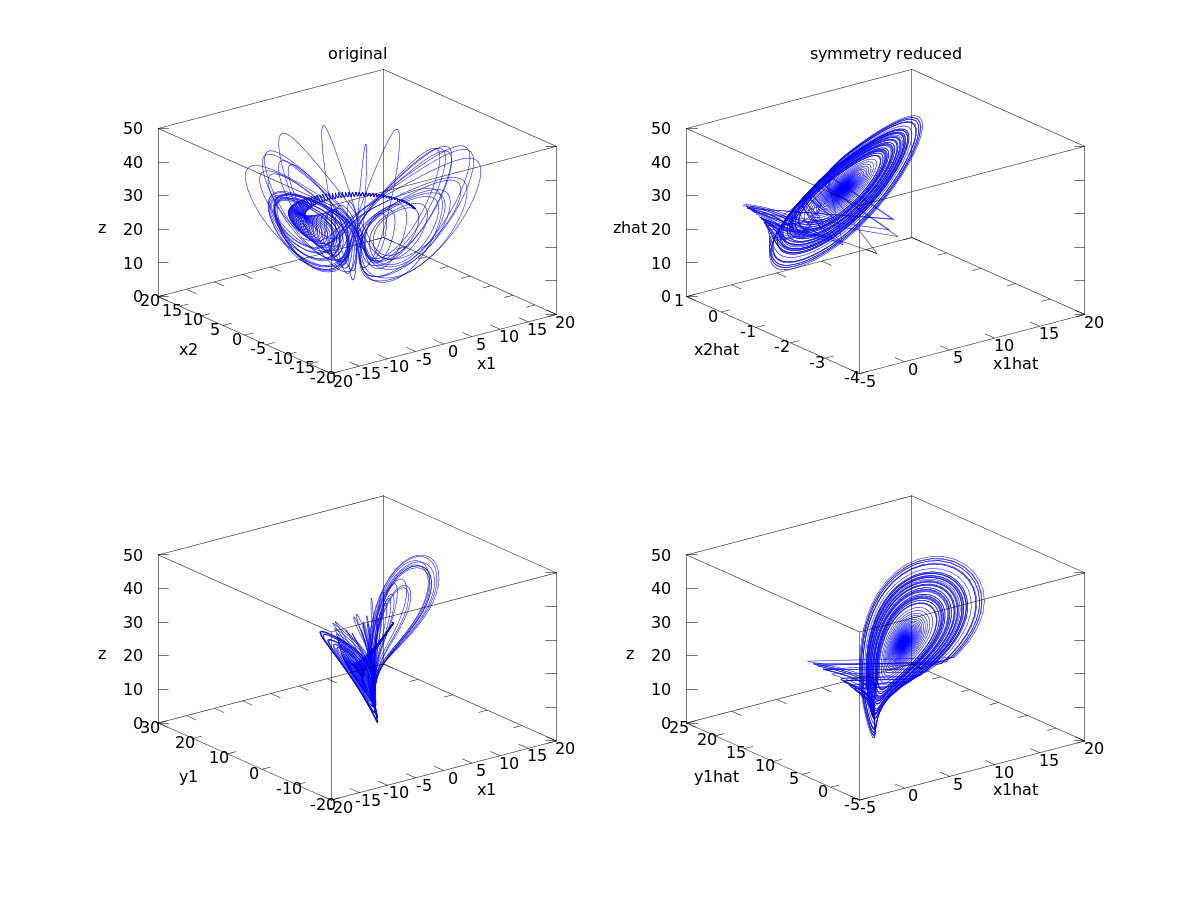
\includegraphics[width=0.9\textwidth]{BBmovingframes}
\end{center}
\caption{ Method of moving frames applied on \cLf.
    }
\label{fig:BBmovingframesCL}
\end{figure}

We can, at least when the symmetry group is abelian, solve the dynamics
on the \reducedsp\ and after that, map it back to the full \statesp\ if
we want to. For the dynamics within the slice, \SOn{2} symmetry we get following
equations:
\bea
  \velRed(\sspRed) &=& \vel(\sspRed) - \dot{\phi} (\sspRed) \groupTan(\sspRed)
\continue
  \dot{\phi}(\sspRed)
    &=& \braket{\vel(\sspRed)}{\sliceTan{}}
    / \braket{\groupTan(\sspRed)}{\sliceTan{}}
\,.
\eea
Here the problem is possibility of getting tangent at the point
$t(\sspRed)$ and the template tangent perpendicular to each other. For
this reason we need multiple, intersecting charts in such a way that this
does not happen. Then we can solve the problem on the
\reducedsp. My unsuccessful attempt of solving reduced dynamics on one
slice:

\begin{figure}[ht]
\begin{center}
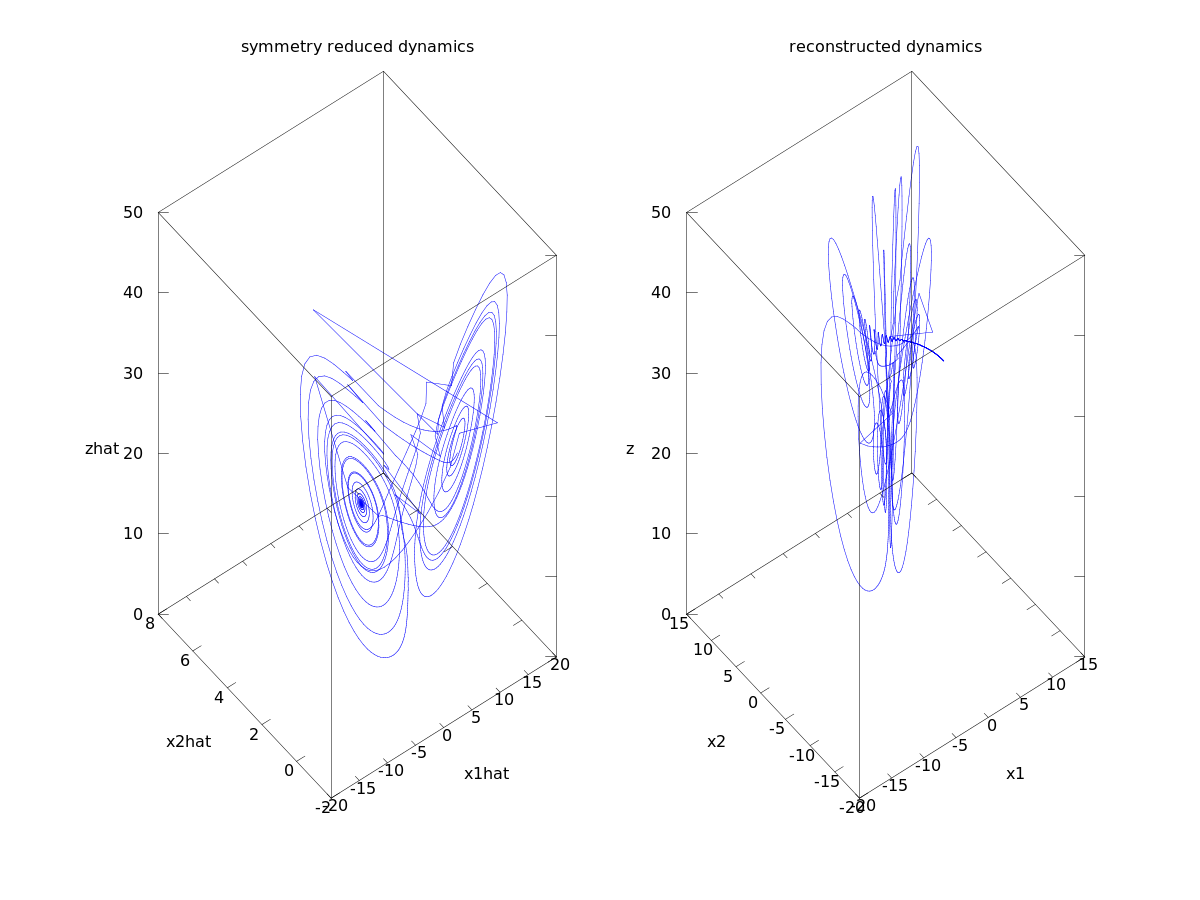
\includegraphics[width=0.9\textwidth]{BBslicedynamics}
\end{center}
\caption{ Dynamics of \cLf\ computed on one slice.
    }
\label{fig:BBslicedynamics}
\end{figure}

\item[2013-07-25  Predrag]
I have edited your formulas using our macros - it does not matter right
now, but it will be handy later, as one uses different notation for ODE
and PDE \statesp s, for example. One has to be precise about the
language, otherwise one ends up with several things being called 'slice',
for example. Definitions are given in Sect.~\emph{V. Charting the slice}
of \refref{atlas12}. A local copy, with all internal comments, is
\HREF{../atlas/atlas12.pdf} {here}.

\refFig{fig:BBmovingframesCL} and \reffig{fig:BBslicedynamics} look
a bit buggy, but basically right - instead of computing \cLf\ one more
time, how about giving a try to \twoMode\ $\SOn{2}$-equivariant flow,
defined in the reducesymm/cgang/2modes.tex (you can get it by a click
\HREF{../cgang/2modes.pdf}{here}, provided you had already pdflatex-ed
2modes.tex). Have a look at it, and then meet with Daniel Borrero, 3. floor
Schatz lab, who can walk you through what we had already done and learned
(all in the 2modes.pdf blog). You can play with it for -let's say- two
weeks, see whether you can find an interesting strange attractor worth
slicing. If that does not work out, we'll give up, and go to \KS\ instead,
which is much more important for our overall goals...






\end{description}
\renewcommand{\ssp}{a}
